% SIAM Article Template
\documentclass[review,onefignum,onetabnum]{siamart190516}

% Information that is shared between the article and the supplement
% (title and author information, macros, packages, etc.) goes into
% ex_shared.tex. If there is no supplement, this file can be included
% directly.

% SIAM Shared Information Template
% This is information that is shared between the main document and any
% supplement. If no supplement is required, then this information can
% be included directly in the main document.


% Packages and macros go here
\usepackage{lipsum}
\usepackage{amsfonts}
\usepackage{graphicx}
\usepackage{epstopdf}
\usepackage{algorithmic}
\ifpdf
  \DeclareGraphicsExtensions{.eps,.pdf,.png,.jpg}
\else
  \DeclareGraphicsExtensions{.eps}
\fi

% Add a serial/Oxford comma by default.
\newcommand{\creflastconjunction}{, and~}

% Used for creating new theorem and remark environments
\newsiamremark{remark}{Remark}
\newsiamremark{hypothesis}{Hypothesis}
\crefname{hypothesis}{Hypothesis}{Hypotheses}
\newsiamthm{claim}{Claim}

% Sets running headers as well as PDF title and authors
\headers{KSPHPDDM and PCHPDDM}{P. Jolivet, J. E. Roman, and S. Zampini}

% Title. If the supplement option is on, then "Supplementary Material"
% is automatically inserted before the title.
\title{KSPHPDDM and PCHPDDM: extending PETS\MakeLowercase{c} with advanced Krylov methods and robust multilevel Overlapping Schwarz preconditioners
%\title{KSPHPDDM and PCHPDDM: extending PETS\MakeLowercase{c} with robust Overlapping Schwarz preconditioners and advanced Krylov methods
%\title{KSPHPDDM and PCHPDDM: Two Classes of Adaptive Krylov and Overlapping Schwarz Methods in PETS\MakeLowercase{c}
\thanks{Submitted to the editors DATE.
%\funding{This work was funded by the Fog Research Institute under contract no.~FRI-454.}
}}

% Authors: full names plus addresses.
\author{Pierre Jolivet\thanks{CNRS, IRIT--ENSEEIHT, Toulouse, France 
  (\email{pierre.jolivet@enseeiht.fr}).}
\and Jose E. Roman\thanks{Universitat Polit\`ecnica de Val\`encia, Val\`encia, Spain
  (\email{jroman@dsic.upv.es}).}
\and Stefano Zampini\thanks{King Abdullah University of Science and Technology, Thuwal, Saudi Arabia 
  (\email{stefano.zampini@kaust.edu.sa}).}}

\usepackage{amsopn}
\DeclareMathOperator{\diag}{diag}


%%% Local Variables: 
%%% mode:latex
%%% TeX-master: "ex_article"
%%% End: 


% Optional PDF information
\ifpdf
\hypersetup{
  pdftitle={KSPHPDDM and PCHPDDM: Extending PETSc with Robust Overlapping Schwarz Preconditioners and Advanced Krylov Methods},
  pdfauthor={P. Jolivet, J. E. Roman, and S. Zampini}
}
\fi

% The next statement enables references to information in the
% supplement. See the xr-hyperref package for details.

% \externaldocument{supplement}

% FundRef data to be entered by SIAM
%<funding-group specific-use="FundRef">
%<award-group>
%<funding-source>
%<named-content content-type="funder-name">
%</named-content>
%<named-content content-type="funder-identifier">
%</named-content>
%</funding-source>
%<award-id> </award-id>
%</award-group>
%</funding-group>
\newcommand\col{:}
\newcommand{\pk}[1]{\texttt{#1}}
\usepackage{stmaryrd}
\usepackage{pgfplotstable}
\pgfplotsset{compat=newest}
\pgfplotsset{colormap={paraview}{rgb(0cm)=(0.278431,0.278431,0.858824) rgb(0.1428571429cm)=(0,0,0.360784) rgb(0.2857142857cm)=(0,1,1) rgb(0.4285714286cm)=(0,0.501961,0) rgb(0.5714285714cm)=(1,1,0) rgb(0.7142857143cm)=(1,0.380392,0) rgb(0.8571428571cm)=(0.419608,0,0) rgb(1cm)=(0.878431,0.301961,0.301961)}}
\usepackage{fancyvrb}
\usepackage{subfig}
\usepackage{upquote,textcomp}
\newcommand*{\fvtextcolor}[2]{\textcolor{#1}{#2}}
\usepackage{colortbl,booktabs}
\definecolor{last}{RGB}{44,123,182}
\definecolor{blueaccent}{RGB}{215,25,28}
\definecolor{myyellow}{RGB}{102,102,17}
\definecolor{myred}{RGB}{197,65,0}
\definecolor{myblue}{RGB}{0,0,235}
\definecolor{myaqua}{RGB}{9,156,156}
\definecolor{mygreen}{RGB}{63,126,28}
\definecolor{paraviewred}{rgb}{0.278431,0.278431,0.858824}
\definecolor{paraviewblue}{rgb}{0.878431,0.301961,0.301961}
\definecolor{darkgray}{RGB}{253,174,97}
\definecolor{mediumgray}{RGB}{255,255,191}
\usepackage[outline]{contour}
\usepackage{tikz}
\usepackage[binary-units=true]{siunitx}
\usetikzlibrary{decorations.text,arrows.meta,calc,plotmarks,shadows,spy,fixedpointarithmetic,patterns,intersections,arrows.meta,shapes,decorations.text,decorations.pathmorphing,backgrounds,fit,positioning,shapes.symbols,chains,3d,calc,external}
\pgfdeclarelayer{background}
\pgfdeclarelayer{foreground}
\pgfsetlayers{background,main,foreground}
\long\def\ifnodedefined#1#2#3{%
    \@ifundefined{pgf@sh@ns@#1}{#3}{#2}%
}
\makeatother
\usepackage{amsmath,etoolbox}
\AtBeginEnvironment{pmatrix}{\setlength{\arraycolsep}{2pt}}
\pgfmathsetmacro{\dof}{4}
\pgfmathsetmacro{\overlap}{1}
\begin{document}

\maketitle

% REQUIRED
\begin{abstract}
  Contemporary applications in computational science and engineering often
    require the solution of linear systems which may be of different sizes,
    shapes, and structures. The goal of this paper is to explain how two
    libraries, PETSc and HPDDM, have been interfaced together in order to offer
    end-users robust overlapping Schwarz preconditioners and advanced Krylov
    methods featuring recycling and block solution techniques.
    The flexibility of the implementation %, which for example may deal with various matrix formats,
    is showcased and explained with minimalist, easy-to-run and reproducible examples
    ranging from {\color{red}fracture mechanics to linear stability analysis}
    to ease the integration of these algorithms into more advanced frameworks.
\end{abstract}

% REQUIRED
\begin{keywords}
  Krylov methods, domain decomposition preconditioners, distributed computing
\end{keywords}

% REQUIRED
\begin{AMS}
  35Q68, 65Y05
\end{AMS}

\section{Introduction}
Implementing and maintaining robust and scalable applications is highly relevant
in the field of computational science and engineering. The efficient production of
such applications requires a rich ecosystem of state-of-the-art reusable libraries
\cite{Bartlett:2017:XFT}. In this paper, we focus on the interoperability of two such libraries.

On the one hand, PETSc \cite{balay1997cient}, the
Portable and Extensible Toolkit for Scientific computation, is a
well-established, actively developed software from the community. It may be used to efficiently
discretize partial differential equations and solve algebraic linear or
nonlinear systems of time-dependent equations. Among its strengths, it offers many
advanced features regarding preconditioning and tailored matrix formats, and it can
interact with third-party libraries, such as
\emph{hypre}~\cite{falgout2002hypre} for linear solvers, TetGen~\cite{si2013tet}
for mesh generation, p4est~\cite{BursteddeWilcoxGhattas11} for adaptive mesh
refinement, to cite a few. The extensibility and robustness of the framework
convinced computational scientists to use PETSc as one of the discretization and/or algebraic backend in
many different higher-level projects, see \url{https://www.mcs.anl.gov/petsc} for a comprehensive list.

On the other hand, HPDDM~\cite{jolivet2013scalable}, the High-Performance unified framework for Domain Decomposition Methods (HPDDM)
is a much smaller project focusing on robust and scalable domain decomposition
preconditioners and advanced iterative
methods~\cite{jolivet2016block} which can efficiently deal with linear
systems with multiple right-hand sides, also known and as block iterative methods,
and when there is a recurrence of varying coefficient matrices and right-hand
sides, recycling iterative methods.

% Htool ?
Here, we describe the integration of the entire HPDDM suite, its advanced iterative
methods and its domain decomposition preconditioners, into PETSc.
The design principles of the interface are showcased considering % alongside
minimalist and easy-to-run examples. Necessary command line
options are provided to:
\begin{itemize}
    \item fulfill reproducibility requirements as advocated by the
Association for Computing Machinery
\url{https://www.acm.org/publications/policies/artifact-review-badging};
    \item ease the integration of these algorithms into more advanced frameworks;
    \item analyze performance results~\cite{hoefler2015scientific}.
\end{itemize}

The paper is divided in two main parts {\color{red} COMPLETE WITH MORE DETAILS WHEN PAPER IS COMPLETED}:
\cref{sec:KSPHPDDM} introduces \pk{KSPHPDDM}, provides applications within an eigensolver
framework and discuss the readiness of the PETSc library in delivering highly efficient block Krylov methods.
\cref{sec:PCHPDDM} introduces \pk{PCHPDDM}. Eventually, concluding remarks may be found
\cref{sec:conclusion}. All PETSc keywords and options are typeset in a \texttt{typewriter} font, these
are public and documented at \url{https://www.mcs.anl.gov/petsc/petsc-master/docs}.

\section{KSPHPDDM}\label{sec:KSPHPDDM}
  \subsection{Related work}
Krylov subspace methods are widely used in numerical linear algebra for solving
linear systems of equations because of their memory efficiency~\cite{barrett1994templates}.
They mainly rely on matrix--vector
operations such as multiplications or transpose multiplications and,
for robust convergence when dealing with challenging high-dimensional systems,
on the application of appropriate preconditioners.
PETSc, as of version 3.14.0, already offers 44 different types of
Krylov methods within the \pk{KSP} base class. Some of the
most used types are \pk{KSPGMRES}, \pk{KSPCG}, or \pk{KSPBCGS}, which respectively implement
the generalized minimal residual method~\cite{saad1986gmres}~(GMRES), conjugate
gradient~\cite{hestenes1952methods}~(CG), or biconjugate gradient stabilized method~\cite{van1992bi}~(BCGS). % Some of these methods are also
% available in other linear algebra backends such as~\emph{hypre} or DUNE~\cite{bastian2010generic}.

Because Krylov methods may need long-term recurrences to mitigate round-off
errors during the generation of subspaces, it is common to introduce a
restart parameter in order to control their memory consumption and the volume of
global communications needed when orthonormalizing a candidate basis vector. Such
restarts may hinder convergence of iterative methods, and even introduce
convergence plateaus. Recycling techniques have been introduced to attenuate
these effects. In PETSc, the Loose GMRES~\cite{baker2005technique}~(LGMRES) and the
Deflated GMRES~\cite{erhel1996restarted,wakam2013158}~(DGMRES), implemented as
\pk{KSPLGMRES} and \pk{KSPDGMRES}, are available. However, neither handle variable
preconditioning, and \pk{KSPDGMRES} does not support complex arithmetic. {\color{red} Also note
that when solving a sequence of linear systems $A_i x_i = b_i, i = 1, 2,
\ldots$, it is not trivial to extend the theory of these methods to perform
recycling throughout both the restarts and the different systems. The
generalized conjugate residual method with inner orthogonalization and deflated
restarting~\cite{parks2006recycling}~(GCRODR) does not suffer from this
limitation.}

% Recycling put aside,
Another important aspect of Krylov methods is their ability
to deal with multiple right-hand sides simultaneously.
Block Krylov methods~\cite{gutknecht2006block} are
designed for solving linear systems $A X = B$, where
$X$ and $B$ are tall-and-skinny matrices with $k \geq 1$ columns.
Such methods, while having higher arithmetic
intensities, generate larger subspaces and typically converge in fewer iterates.

These methods are not currently offered in PETSc and they are
less frequently implemented in general purpose libraries because they require
somehow more involved kernels such as matrix--matrix multiplication, instead of
matrix--vector, and may involve different inner-product realizations~\cite{frommer2017block}.
Still, systems with multiple right-hand sides are ubiquitous,
e.g., in tomography~\cite{tournier2016micro}, data
analytics~\cite{KALANTZIS2018136}, eigensolvers~\cite{knyazev2001toward}, geophysics~\cite{calandra2012flexible}, quantum chromodynamics~\cite{sakurai2010application}, and optimization with time-dependent partial differential equations as constraints.
% Of course, it is possible to cast a system with multiple right-hand sides into a sequence of systems with the same coefficient matrix but changing right-hand sides $A x_i = b_i, i = 1,2,\ldots,k$. However,

Trilinos~\cite{heroux2005overview} is another well-known software for scientific
computing and it provides iterative methods through its Belos package~\cite{bavier2012amesos2}.
Although having PETSc and
Trilinos interoperate is possible, there is currently no \pk{KSP} interface to Belos. % This limits its composability inside complete PETSc applications.
Furthermore, some of the Krylov methods implemented in
HPDDM and discussed in ~\cref{sec:interface-ksp}, are not available in Belos.

  \subsection{Interfacing HPDDM Krylov methods in PETSc\label{sec:interface-ksp}}\
In this section, we provide details of the
interface between HPDDM Krylov methods and the various PETSc
classes. It is assumed that the right-hand sides, and
consequently the solutions, are always dense vectors or matrices.

\pk{KSPHPDDM}, the interface between HPDDM Krylov methods and PETSc, is automatically
registered since PETSc version 3.12 when configuring PETSc with the extra
flag \pk{-{}-download-hpddm}. HPDDM linear solvers can be selected using the command
line option \pk{-ksp\_type hpddm}, or the routine \pk{KSPSetType}(ksp,
\pk{KSPHPDDM}), and the following Krylov methods can be accessed:
\begin{itemize}
    \item pseudo-block GMRES or flexible GMRES~\cite{saad1993flexible};
    \item pseudo-block CG or flexible CG~\cite{notay2000flexible};
    \item pseudo-block GCRODR or flexible GCRODR~\cite{carvalho2011flexible};
    \item block GMRES or flexible GMRES~\cite{calandra2012flexible}, with deflation at each restart;
    \item block CG~\cite{o1980block};
    \item breakdown-free block CG~\cite{ji2017breakdown}, with deflation at each iteration;
    \item block GCRODR or flexible GCRODR, with deflation at each restart.
\end{itemize}
While being mathematically equivalent to
their ``standard'' counterparts, the pseudo-block variants try to fuse together multiple similar
operations like matrix--vector
products to achieve higher arithmetic intensity, or to decrease the
number of global synchronizations needed for scalar products.
HPDDM Krylov methods may be selected {\color{red} TODO API FOR KSPHPDDMSetVariant?} using the
options \pk{-ksp\_hpddm\_type}
\pk{(gmres$|$cg$|$gcrodr$|$bgmres$|$bcg$|$bfbcg$|$bgcrodr$|$preonly)}, or the
routine \pk{KSPHPDDMSetType}(ksp, \pk{KSPHPDDMType}).
Preconditioning variants can be specified via
\pk{-ksp\_hpddm\_variant} \pk{(left$|$right$|$flexible)} to select whether the
preconditioner is applied on the left, on the right, or if it cannot be
represented as a linear operator. In this latter case, the preconditioner is
always applied on the right, except for FCG. HPDDM CG
and its variants BCG and BFBCG only handle left-preconditioning.  It is also
possible to set the preconditioning side through the more common PETSc option
\pk{-ksp\_pc\_side (left$|$right)}.  Finally, convergence monitoring with the
\pk{KSPMonitor} interface is fully supported, as well as the specification of
customized convergence testing via the \pk{KSPSetConvergenceTest} callback.

According to the standard PETSc notation, ksp($A$, $P_{A'}$)
defines a \pk{KSP} used to solve a system $Ax=b$ using a preconditioner $P_{A'}$ built
using an operator $A'$ which is usually, but not necessarily, equal to $A$. While solving
the linear system via \pk{KSPSolve}(ksp, $b$, $x$) or \pk{KSPMatSolve}(ksp, $B$, $X$),
HPDDM will repeatedly call the following PETSc routines:
\begin{itemize}
    \item \pk{MatMult}($A$, $x$, $y$) for $y = Ax$;
    \item \pk{MatMatMult}($A$, $X$, {\small \pk{MAT\_REUSE\_MATRIX}}, {\small
        \pk{PETSC\_DEFAULT}}, $Y$)\footnote{or \pk{MatProductNumeric}($Y$) with PETSc 3.14.0 and above} for $Y =
        AX$;
    \item \pk{PCApply}($P_{A'}$, $x$, $y$) for $y = P_{A'}x$;
    \item \pk{PCMatApply}($P_{A'}$, $X$, $Y$) for $Y = P_{A'}X$;
\end{itemize}
As of version 3.14.0, PETSc provides unified routines for applying $A$ or $P_{A'}$
to a tall-and-skinny dense matrix $X$. However, when no specialized implementation
is available, PETSc will loop over the columns of $X$ and successively apply $A$
or $P_{A'}$ to get all columns of $Y$. For matrix--matrix products, there are
currently specialized implementations for the following \pk{MatType}:
\begin{itemize}
    \item \pk{MatSeqAIJ}, standard sequential sparse matrix, based on compressed sparse row format;
    \item \pk{MatSeqBAIJ}, block sparse matrix, based on block compressed sparse row format;
    \item \pk{MatSeqSBAIJ}, symmetric block sparse matrix stored in upper triangular form.
    \item \pk{MatMPIAIJ}, standard parallel sparse matrix;
    \item \pk{MatShell}, user-defined matrix;
    \item \pk{MatNest}, block-defined matrix with nested submatrices;
    \item \pk{MatSeqAIJCUSPARSE}, standard sequential sparse matrix, offloaded to a GPU using cuSPARSE~\cite{cusparse-web-page}.
\end{itemize}
The following preconditioners have specialized implementations for dealing
efficiently with multiple vectors:
\begin{enumerate}
    \item \pk{PCNONE}: $P_{A'} = I$, identity matrix;
    \item \pk{PCKSP}: embedded Krylov method inside $P_{A'}$;
    \item \pk{PCMAT}: multiplication by $A'$, i.e., $P_{A'} = {A'}$;
    \item \pk{PCSHELL}: user-defined preconditioner, e.g., matrix-free;
    % \item \pk{PCSPAI}: sparse approximate inverse~\cite{grote1997parallel};
    \item \pk{PCHARA}~\cite{10.1145/3232850};
    \item \pk{PCHPDDM}: see~\cref{sec:PCHPDDM};\label{it:hpddm}
    \item \pk{PCASM} and \pk{PCGASM}: overlapping Schwarz methods;\label{it:asm}
    \item \pk{PCBJACOBI}: block Jacobi;\label{it:bjacobi}
    \item \pk{PCLU} or \pk{PCCHOLESKY}: exact $LU$ or Cholesky factorization,
        e.g., $P_{A'} = {U}^{-1}{L}^{-1}$;\label{it:lu}
    \item \pk{PCILU} or \pk{PCICC}: incomplete $LU$ or Cholesky
        factorization.\label{it:ilu}
\end{enumerate}
One appealing feature of domain decomposition-like preconditioners 
\cref{it:hpddm,it:asm,it:bjacobi} is that they most often rely on exact or inexact
factorizations~\cref{it:lu,it:ilu} as subdomain solvers.
In these cases, it is possible to access the so-called local or distributed factored matrix $F$
%via \pk{PCFactorGetMatrix} and then call \pk{MatMatSolve}($F$, $\tilde{Y}$, $\tilde{X}$).
via \pk{PCFactorGetMatrix}, and then call \pk{MatMatSolve}($F$, $X$, $Y$) to take advantage
of blocked forward eliminations and backward substitutions from the various factorization packages
interfaced with PETSc. In the case of a sparse coefficient matrix $A'$,
this strategy is possible with: MUMPS~\cite{amestoy2001fully},
SuiteSparse~\cite{davis2004algorithm}, MKL
PARDISO or CPARDISO~\cite{mkl-web-page}, and SuperLU~\cite{li2005overview} or
SuperLU\_DIST~\cite{li2003superlu_dist}. For the case of a dense coefficient
matrix $A'$: ScaLAPACK and Elemental~\cite{poulson2013elemental}. 
Future work will consider extending the various implementations of PETSc
preconditioning infrastructure to increase the arithmetic intensity of the
block preconditioner application phase.

The rest of the operations are then performed directly inside HPDDM.
Specifically, within Krylov methods using the Arnoldi process, or when recycling is requested,
one has to compute $QR$ factorizations of tall-and-skinny dense matrices to orthonormalize
candidate basis vectors. Such operations are performed using the CholQR algorithm~\cite{stathopoulos2002block}, or
via the (modified) Gram--Schmidt method.
For Hessenberg matrices generated by the Arnoldi
process, it is common to update their $QR$ decomposition using Givens
rotations~\cite{saad2003iterative}. For block Hessenberg matrices, Householder reflectors are
used instead~\cite{gutknecht2008updating}.
These orthonormalization variants can be selected at runtime with the option \pk{-ksp\_hpddm\_qr (cholqr$|$mgs$|$cgs)}. {\color{red} API?}

    \subsubsection{User-defined deflation space} Recycling Krylov methods try to
extract convergence information by solving a small standard or a generalized
dense eigenproblem at the end of each cycle or when convergence is reached, and
then reuse it appropriately for subsequent
solves~\cite{saad2000deflated,stathopoulos2009deflation,soodhalter2014krylov}.
The routine \pk{KSPHPDDMGetDeflationSpace} can be used to retrieve such deflation subspaces, stored as distributed
dense tall-and-skinny matrices. It is also possible to provide this information
via \pk{KSPHPDDMSetDeflationSpace} in case end-users already know a good initial
deflation subspace.

%     \subsubsection{MatKAIJ and systems with multiple right-hand sides\label{sec:matkaij}}
% {\color{red} TODO: move KSPMatSolve discussion out, and clean up the section, add results for irk?}
% There is a wide range of available matrix types in PETSc. One of them is
% \pk{MatKAIJ}, for which it is assumed that an operator may be written as $I \otimes S
% + A \otimes T$, with $S$ and $T$ elements of $\mathbb{K}^{p\times q}$ and
% $A$ a standard sparse matrix of dimension $n$. If $p=q=k$, $S = \lambda I$, and $T =
% \mu I$, then solving $(I \otimes S + A \otimes T) x = b$ may be cast into a
% system with multiple right-hand sides $(\lambda I + \mu A)X = B$ where $B$ is
% the row-major representation of $b$, i.e., $b_{k \cdot i + j} = B_{i, j},
% \forall (i, j) \in \llbracket 1;n\rrbracket \times \llbracket 1;k\rrbracket$.
% On the one hand, due to the structure of the operator, it is challenging to
% define appropriate preconditioners for $(I \otimes S + A \otimes T)$: only
% \pk{PCPBJACOBI} is currently implemented for \pk{MatKAIJ}. On the other hand,
% it may be simpler to efficiently approximate the inverse of $A$. In
% \pk{KSPHPDDM}, the type of the operators is checked and if it is \pk{MatKAIJ},
% the single right-hand side system is automatically cast into a system with
% multiple right-hand sides instead. % The standard function \pk{KSPSolve} takes as input argument a \pk{KSP} and two \pk{Vec}.
% A new function \pk{KSPMatSolve} was added in PETSc 3.14.0, which takes as input argument
% a \pk{KSP} and two dense \pk{Mat}, for solving true
% multiple right-hand side systems. If the input \pk{KSP} is not of type
% \pk{KSPHPDDM}, the solution phase is done in a column by column fashion.
% Otherwise, it is possible to use any \pk{KSPHPDDM} \mbox{(pseudo-)block} Krylov methods.
% Furthermore, a function \pk{KSPSetMatSolveBlockSize} is also provided to decompose
% a single large block of column vectors into multiple sub-blocks.
% \pk{KSPMatSolve} is then called repeatedly until all sub-blocks are traversed.
% This was inspired by MUMPS~\cite{amestoy2001fully} option
% ICNTL(27)\footnote{\url{http://mumps.enseeiht.fr/doc/userguide_5.3.1.pdf}, section 6.1}.
    \subsubsection{Systems with multiple right-hand sides\label{sec:kspmatsolve}}
Along with \pk{PCMatApply} introduced in PETSc 3.14.0, a new function
\pk{KSPMatSolve} was added for solving systems with multiple right-hand sides.
It takes as input argument a \pk{KSP} and, just as for \pk{PCMatApply}, two
dense \pk{Mat}. If the input \pk{KSP} is not of type \pk{KSPHPDDM}, the
solution phase is done in a column by column fashion.  Otherwise, it is
possible to use any \pk{KSPHPDDM} \mbox{(pseudo-)block} Krylov methods.
Furthermore, a function \pk{KSPSetMatSolveBlockSize} is also provided to
decompose a single large block of column vectors into multiple sub-blocks.
\pk{KSPMatSolve} is then called repeatedly until all sub-blocks are traversed.
This was inspired by MUMPS~\cite{amestoy2001fully} option
ICNTL(27)\footnote{\url{http://mumps.enseeiht.fr/doc/userguide_5.3.3.pdf},
section 6.1}.

With these added functions, it is now possible to do code refactorization for
applications that deal with multiple right-hand sides.  As a striking example,
LOBPCG~\cite{knyazev2001toward} or CISS~\cite{sakurai2003projection}
implementations in SLEPc~\cite{hernandez2005ssf}, the Scalable Library for
Eigenvalue Problem computations built on top of PETSc, were previously not
using blocking when applying the preconditioner or solving linear systems. This has been rewritten for version 3.14.0 and the benefit of
this new implementation is displayed in~\cref{sec:lobpcg}.

As a side note, when dealing with
\pk{MatKAIJ} matrices, for which it is assumed that an operator may be written as $I \otimes S
+ A \otimes T$, with $S$ and $T$ elements of $\mathbb{K}^{p\times q}$ and
$A$ a standard sparse matrix of dimension $n$, it is also possible to use block Krylov methods. 
Indeed, if $p=q=k$, $S = \lambda I$, and $T =
\mu I$, then solving $(I \otimes S + A \otimes T) x = b$ may be cast into a
system with $k$ right-hand sides $(\lambda I + \mu A)X = B$ where $B$ is
the row-major representation of $b$, i.e., $b_{k \cdot i + j} = B_{i, j},
\forall (i, j) \in \llbracket 1;n\rrbracket \times \llbracket 1;k\rrbracket$.
On the one hand, due to the structure of the operator, it is challenging to
define appropriate preconditioners for $(I \otimes S + A \otimes T)$: only
\pk{PCPBJACOBI} is currently implemented for \pk{MatKAIJ}. On the other hand,
it may be simpler to efficiently approximate the inverse of $A$. In
\pk{KSPHPDDM}, the type of the operators is checked: if it is \pk{MatKAIJ} and
the previous condition on $p, q, S$, and $T$ is fulfilled, the single
right-hand side system is automatically cast into a system with multiple
right-hand sides instead.

  \subsection{Applications and numerical results}
    \subsubsection{Reproducibility of the results from Parks et
    al.~\cite{parks2006recycling}}
Alongside the paper introducing GCRODR~\cite{parks2006recycling},
a MATLAB implementation was provided and is since then
available\footnote{\url{https://www.sandia.gov/~mlparks/GCRODR.zip}}. It comes
with a sequence of ten ``linear systems from a finite element fracture mechanics
problem constructed by Philippe H.\ Geubelle and Spandan Maiti." The goal of
this paragraph is to explain how the results have been reproduced in PETSc.
The dataset and the source code are available at
\url{https://gitlab.com/petsc/datafiles/-/tree/master/matrices/hpddm/GCRODR}
and
\url{https://www.mcs.anl.gov/petsc/petsc-master/src/ksp/ksp/tutorials/ex75.c.html}
respectively. In order to check the correctness of the \pk{KSPHPDDM} interface,
the following tests are performed:
\begin{itemize}
    \item in MATLAB, unpreconditioned GCRODR(40, 20), ICC(0) left-preconditioned
        GCRODR(40, 20), and Jacobi right-preconditioned GCRODR(40, 20);
    \item in PETSc with unpreconditioned and unrestarted GMRES($\infty$) \pk{KSPGMRES};
    \item in PETSc with \pk{KSPHPDDM}, all of the above.
\end{itemize}
The notation GCRODR($n$, $m$) indicates a restart after $n$ iterations and a recycling subspace of dimension $m$.
In all the cases, convergence is declared when the initial unpreconditioned residual is reduced by 10 orders of magnitude.
Except for the right-preconditioned GCRODR, these tests are the same as the
ones from the original GCRODR paper~\cite{parks2006recycling}.
All PETSc tests are performed using four MPI
processes and they can be launched using the following command lines: \\[-4pt]
\begin{Verbatim}[fontsize=\footnotesize,frame=single,framerule=0.1mm,commandchars=&\[\]]
&fvtextcolor[mygreen][$] &fvtextcolor[myyellow][mpirun] -n 4 ./ex75 -ksp_converged_reason -pc_type none -ksp_rtol 1e-10             &fvtextcolor[myred][\]
  -ksp_type hpddm -ksp_hpddm_type gcrodr -ksp_gmres_restart 40 -ksp_hpddm_recycle 20 &fvtextcolor[myred][\]
  -load_dir &fvtextcolor[myyellow][${DATAFILESPATH}]/matrices/hpddm/GCRODR
&fvtextcolor[mygreen][$] &fvtextcolor[myyellow][mpirun] -n 4 ./ex75 -ksp_converged_reason -redundant_pc_type icc -ksp_rtol 1e-10    &fvtextcolor[myred][\]
  -ksp_type hpddm -ksp_hpddm_type gcrodr -ksp_gmres_restart 40 -ksp_hpddm_recycle 20 &fvtextcolor[myred][\]
  -load_dir &fvtextcolor[myyellow][${DATAFILESPATH}]/matrices/hpddm/GCRODR -pc_type redundant
&fvtextcolor[mygreen][$] &fvtextcolor[myyellow][mpirun] -n 4 ./ex75 -ksp_converged_reason -pc_type jacobi -ksp_rtol 1e-10           &fvtextcolor[myred][\]
  -ksp_type hpddm -ksp_hpddm_type gcrodr -ksp_gmres_restart 40 -ksp_hpddm_recycle 20 &fvtextcolor[myred][\]
  -ksp_pc_side right -load_dir &fvtextcolor[myyellow][${DATAFILESPATH}]/matrices/hpddm/GCRODR
&fvtextcolor[mygreen][$] &fvtextcolor[myyellow][mpirun] -n 4 ./ex75 -ksp_converged_reason -pc_type none -ksp_rtol 1e-10             &fvtextcolor[myred][\]
  -ksp_type hpddm -ksp_gmres_restart 500                                             &fvtextcolor[myred][\]
  -load_dir &fvtextcolor[myyellow][${DATAFILESPATH}]/matrices/hpddm/GCRODR
\end{Verbatim}
For the case of ICC(0), a \pk{PCREDUNDANT} is needed as well since
PETSc does not provide a parallel ICC solver. The iteration numbers
needed to reach convergence are gathered in~\cref{fig:comparison}.  The
cases \ref{pgfplots:r0} and
\ref{pgfplots:r1} (resp. \ref{pgfplots:r6} and \ref{pgfplots:r7}) reproduce Figure 4.2 in~\cite{parks2006recycling}.
We note here that the results obtained with
\pk{PCICC} from PETSc \ref{pgfplots:r3} and ichol from MATLAB \ref{pgfplots:r2}, which uses SuiteSparse, are not consistent.
%Apart from
%the tests \ref{pgfplots:r2} and \ref{pgfplots:r3} using $ICC(0)$ and \ref{pgfplots:r4} and \ref{pgfplots:r5}
%using the Jacobi method, one may notice that \ref{pgfplots:r0} and
%\ref{pgfplots:r1} (resp. \ref{pgfplots:r6} and \ref{pgfplots:r7}) are almost a
%perfect match and reproduce partially Figure 4.2 from Parks et
%al.~\cite{parks2006recycling}.
\pgfplotstableread{
sys none-matlab icc-matlab jacobi-matlab none-hpddm icc-hpddm jacobi-hpddm icc-gmres none-gmres icc-petsc none-petsc
401 498         293        457           497        94        460          127       438        127       438
402 228         125        187           231        37        184          127       449        127       449
403 209         113        182           206        34        177          127       450        127       450
404 199         112        175           198        33        174          127       450        127       450
405 198         110        174           198        34        172          127       451        127       451
406 198         111        174           199        34        174          127       452        127       452
407 206         114        180           206        33        179          126       458        126       458
408 207         115        181           208        34        182          128       458        135       458
409 207         110        181           207        34        181          128       458        128       458
410 206         110        179           206        34        179          128       457        128       457
}\loadedtable
    \begin{figure}
\centering \begin{tikzpicture}
    \begin{axis}[xlabel=System index,ylabel={\# of iterations},xmin=401,xmax=410,ymin=0,ymajorgrids,
        legend columns=1,enlarge x limits=0.05,
        legend style={font=\small,at={(1.02,0.5)},anchor=west, legend cell align=left}]
\addplot[very thick,myred]                       table[x expr=\thisrowno{0},y expr=\thisrowno{1}, col sep=space] {\loadedtable};\label{pgfplots:r0}
\addplot[very thick,mark=*,only marks,myred]     table[x expr=\thisrowno{0},y expr=\thisrowno{4}, col sep=space] {\loadedtable};\label{pgfplots:r1}
\addplot[very thick,myaqua]                      table[x expr=\thisrowno{0},y expr=\thisrowno{2}, col sep=space] {\loadedtable};\label{pgfplots:r2}
\addplot[very thick,mark=pentagon*,only marks,myaqua]    table[x expr=\thisrowno{0},y expr=\thisrowno{5}, col sep=space] {\loadedtable};\label{pgfplots:r3}
\addplot[very thick,myyellow]                    table[x expr=\thisrowno{0},y expr=\thisrowno{3}, col sep=space] {\loadedtable};\label{pgfplots:r4}
\addplot[very thick,mark=square*,only marks,myyellow]  table[x expr=\thisrowno{0},y expr=\thisrowno{6}, col sep=space] {\loadedtable};\label{pgfplots:r5}
\addplot[very thick,last]                      table[x expr=\thisrowno{0},y expr=\thisrowno{10}, col sep=space]{\loadedtable};\label{pgfplots:r6}
\addplot[very thick,mark=triangle*,only marks,last]    table[x expr=\thisrowno{0},y expr=\thisrowno{8}, col sep=space] {\loadedtable};\label{pgfplots:r7}
\legend{{MATLAB unpreconditioned GCRODR},{\pk{KSPHPDDM}},% unpreconditioned GCRODR(40, 20)},
        {MATLAB $ICC(0)$-preconditioned GCRODR},{\pk{KSPHPDDM}},% $ICC(0)$-preconditioned GCRODR(40, 20)},
        {MATLAB Jacobi-preconditioned GCRODR},{\pk{KSPHPDDM}},% Jacobi-preconditioned GCRODR(40, 20)},
        {Unpreconditioned \pk{KSPGMRES}},{\pk{KSPHPDDM}}}% unpreconditioned GMRES($\infty$)}}
\end{axis}
\end{tikzpicture}
        \caption{\# of iterations needed to converge for various
        configurations as originally tested by Parks et
        al.~\cite{parks2006recycling}. Note that \pk{PCICC} and
        \textnormal{ichol} from MATLAB are not consistent, hence the discrepancy
        between \ref{pgfplots:r2} and \ref{pgfplots:r3}. In the other cases,
        the numbers of iterations needed by KSPHPDDM match with the respective
        MATLAB or PETSc reference implementation.\label{fig:comparison}}
    \end{figure}
    \subsubsection{Linear stability analysis}
In this section, we apply recycling Krylov methods in the context of linear
stability analysis and consider the solution of the following generalized eigenvalue problem:
\begin{equation}\label{eq:lsa}
    J(q_b)x = \lambda \begin{bmatrix}M & 0 \\ 0 & 0 \end{bmatrix} x,
\end{equation}
where $J$ is the Jacobian of the incompressible steady-state Navier--Stokes equation
evaluated using a given base flow $q_b = \begin{bmatrix}u_b \\ p_b\end{bmatrix}$ and
$M$ the discretization of the mass matrix on the space of velocities. Interested
readers are referred to~\cite{moulin2018al} for more details and for larger
runs.

The mini-app employed for the numerical results is built on top of
FreeFEM~\cite{hecht2012new} and it is available at
\url{https://github.com/prj-/moulin2019al}. As eigenvalue solver, it uses
SLEPc, and thus reuses PETSc linear solver infrastructure.

There are different methods to compute the eigenvalues
of~\cref{eq:lsa} near a complex-valued shift $\sigma$. In this paragraph, emphasis will be put
on the Krylov--Schur method~\cite{Stewart2002}, which for interior eigenvalues relies on spectral transformations
and on the solution of successive linear systems such as:
\begin{equation}\label{eq:ks}
    \left(J(q_b) - \sigma \begin{bmatrix}M&0\\0&0\end{bmatrix}\right)x_i = b_i,
\end{equation}
which, in SLEPc, are parameterized using the \pk{-st\_} prefix.
In this work, the above linear system is preconditioned using a modified augmented Lagrangian
approach~\cite{Benzi2011a,moulin2018al}

The effectiveness of subspace recycling is shown for
finding the 5 eigenpairs closest to the shift $\sigma = 10^{-6} + 0.6\mathfrak{i}$ for a
flow past a cylinder at Reynolds 100. Results can be reproduced using the following four commands.
We note here that the first two commands are merely used to generate
the base flow $q_b$ with a \pk{SNES}, a PETSc object used to solve
nonlinear problems, using a continuation method on the Reynolds number. \\[-4pt]
\begin{Verbatim}[fontsize=\footnotesize,frame=single,framerule=0.1mm,commandchars=&\[\]]
&fvtextcolor[mygreen][$] &fvtextcolor[myyellow][mpirun] -n 4 FreeFem++-mpi Nonlinear-solver.edp -Re 50 -v 0
&fvtextcolor[mygreen][$] &fvtextcolor[myyellow][mpirun] -n 4 FreeFem++-mpi Nonlinear-solver.edp -Re 100 -v 0
&fvtextcolor[mygreen][$] &fvtextcolor[myyellow][mpirun] -n 4 FreeFem++-mpi Eigensolver.edp -Re 100 -v 0 -st_ksp_rtol 1.0e-4         &fvtextcolor[myred][\]
  -st_ksp_type fgmres -st_ksp_gmres_restart 200 -st_ksp_converged_reason
&fvtextcolor[mygreen][$] &fvtextcolor[myyellow][mpirun] -n 4 FreeFem++-mpi Eigensolver.edp -Re 100 -v 0 -st_ksp_rtol 1.0e-4         &fvtextcolor[myred][\]
  -st_ksp_type hpddm -st_ksp_gmres_restart 200 -st_ksp_converged_reason              &fvtextcolor[myred][\]
  -st_ksp_hpddm_variant flexible -st_ksp_hpddm_recycle 10 -st_ksp_hpddm_type gcrodr
\end{Verbatim}

The Krylov--Schur algorithm converges in six outer iterations (restarts), with a total of 46 inner solves~\cref{eq:ks}.
Recycling of Krylov subspaces with \pk{KSPHPDDM} provides algorithmic speedup by lowering the number of iterations per inner solve,
as reported in~\cref{fig:comparison-slepc}, from 80 with \pk{KSPFGMRES} to 45.
A similar speedup can be observed in terms of runtime, with the time spent for the solution of the eigenvalue problem being reduced from \SI[round-mode = places,round-precision=1,group-minimum-digits=3,group-separator = {,}]{1509}{\sec} to \SI[round-mode = places,round-precision=1,group-minimum-digits=3,group-separator = {,}]{1052}{\sec}. {\color{red} FIXME LATER: These timings, and all which follow except in~\cref{sec:primitives}, have been obtained on {Ir\`ene}, a system composed of \pgfmathprintnumber[assume math mode=true]{1656} nodes with two 24-core Intel Xeon Platinum 8168 clocked at \SI{2.7}{\giga\hertz}}.
\pgfplotstableread{
sys hpddm fgmres
1   77    77
2   54    83
3   53    83
4   52    81
5   52    81
6   51    78
7   51    79
8   51    80
9   51    80
10  51    77
11  51    79
12  51    79
13  51    79
14  53    77
15  52    79
16  49    78
17  51    77
18  51    79
19  52    79
20  52    79
21  51    77
22  51    78
23  51    79
24  53    80
25  54    79
26  52    79
27  49    75
28  51    78
29  51    78
30  51    77
31  50    78
32  55    81
33  56    79
34  54    80
35  53    80
36  53    78
37  50    78
38  52    79
39  53    77
40  52    77
41  54    80
42  53    80
43  55    80
44  53    79
45  52    77
46  53    80
}\loadedtableSLEPc
    \begin{figure}[!t]
\centering \begin{tikzpicture}
    \begin{axis}[xlabel={Krylov--Schur system index},ylabel={\# of
        iterations},xmin=1,xmax=46,ymin=0,ymajorgrids,
        legend columns=1,enlarge x limits=0.05, height=5.5cm,
        legend style={font=\small,at={(0.98,0.02)}, legend cell align=left,
        anchor=south east}]
\addplot[very thick,last]     table[x expr=\thisrowno{0},y expr=\thisrowno{2}, col sep=space] {\loadedtableSLEPc};\label{pgfplots:m0}
\addplot[very thick,myred,densely dashed]       table[x expr=\thisrowno{0},y expr=\thisrowno{1}, col sep=space] {\loadedtableSLEPc};\label{pgfplots:m1}
\legend{{\pk{KSPFGMRES}},{\pk{KSPHPDDM}}}
\end{axis}
\end{tikzpicture}
        \caption{\# of inner iterations for systems~\cref{eq:ks} with~\ref{pgfplots:m0} or without~\ref{pgfplots:m1} recycling.\label{fig:comparison-slepc}}
    \end{figure}
\pgfplotstableread{
N    baij-1-T    baij-1-F   sbaij-1-T   sbaij-1-F  aij-1-T     aij-1-F    baij-3-T    baij-3-F   sbaij-3-T   sbaij-3-F  aij-3-T     aij-3-F    baij-10-T   baij-10-F  sbaij-10-T  sbaij-10-F aij-10-T    aij-10-F     cusparse-1-T    cusparse-1-F    cusparse-3-T    cusparse-3-F    cusparse-10-T   cusparse-10-F    aijmkl-seq-1-T      aijmkl-seq-3-T      aijmkl-seq-10-T     baijmkl-seq-1-T      baijmkl-seq-3-T      baijmkl-seq-10-T   sbaijmkl-seq-1-T      sbaijmkl-seq-3-T      sbaijmkl-seq-10-T         aijmkl-1-T      aijmkl-3-T      aijmkl-10-T     baijmkl-1-T      baijmkl-3-T      baijmkl-10-T   sbaijmkl-1-T      sbaijmkl-3-T      sbaijmkl-10-T
1      2.0126e-01   1.4696e+08 8.0098e-02   1.4696e+08   9.3388e-02   1.4696e+08     8.9584e-01   1.3535e+09    6.2428e-01   1.3638e+09     1.2072e+00   1.3535e+09   4.0734e+00   5.4450e+09    2.2476e+00   5.4708e+09    5.0428e+00   5.4450e+09   2.1248e-03   1.5211e+08   1.3669e-02   1.3690e+09   4.7833e-02   5.4759e+09   6.6857e-02  7.4649e-01   3.1128e+00   4.7672e-01   6.2903e-01  2.2271e+00   4.7675e-01   6.2990e-01    2.2273e+00    7.8399e-03    8.6487e-02    3.5536e-01   5.2814e-02 6.6225e-02   2.4584e-01   4.5115e-02   6.6404e-02   2.4489e-01
2      3.2635e-01   2.9392e+08 2.4204e-01   3.2482e+08   1.1522e-01   3.0422e+08     1.2835e+00   2.7071e+09    1.0697e+00   2.9234e+09     9.9480e-01   2.7380e+09   1.4504e+01   1.0890e+10    1.5265e+01   1.1694e+10    3.7799e+00   1.0952e+10   5.2164e-03   3.0422e+08   3.4056e-02   2.7380e+09   7.7659e-02   1.0952e+10   1.1703e-01  9.3872e-01   3.5976e+00   4.7905e-01   7.3497e-01  3.3331e+00   4.7886e-01   7.3415e-01    3.3297e+00    1.2450e-02    1.0124e-01    3.9873e-01   4.7633e-02 7.4107e-02   2.8513e-01   4.7733e-02   7.4693e-02   2.8507e-01
8      7.9573e-01   1.1757e+09 1.0070e+00   1.2993e+09   3.3729e-01   1.2169e+09     3.3663e+00   1.0828e+10    3.9830e+00   1.1694e+10     2.4656e+00   1.0952e+10   2.2209e+01   4.3560e+10    2.2545e+01   4.6775e+10    9.2040e+00   4.3807e+10   1.3652e-02   1.2169e+09   8.2139e-02   1.0952e+10   1.8984e-01   4.3807e+10   4.2722e-01  2.8760e+00   1.0913e+01   1.3256e+00   1.7457e+00  7.9644e+00   1.3210e+00   1.7410e+00    7.9679e+00    4.2997e-02    2.6899e-01    1.6814e+00   1.3183e-01 1.7832e-01   8.8593e-01   1.3082e-01   1.7947e-01   8.8420e-01
16     2.1378e+00   2.3513e+09 3.0837e+00   2.5986e+09   6.7295e-01   2.4337e+09     9.1522e+00   2.1656e+10    1.1762e+01   2.3387e+10     4.9326e+00   2.1904e+10   3.1530e+01   8.7120e+10    2.9334e+01   9.3549e+10    1.8462e+01   8.7615e+10   2.4907e-02   2.4337e+09   1.3832e-01   2.1904e+10   3.3609e-01   8.7615e+10   8.5514e-01  5.7493e+00   2.1980e+01   2.6391e+00   3.4887e+00  1.5947e+01   2.6455e+00   3.4893e+00    1.5928e+01    8.4255e-02    5.4284e-01    3.3861e+00   2.6162e-01 3.5777e-01   1.7955e+00   2.6238e-01   3.5880e-01   1.7923e+00
32     4.2781e+00   4.7026e+09 6.5426e+00   5.1972e+09   1.3447e+00   4.8675e+09     1.8545e+01   4.3313e+10    2.4015e+01   4.6775e+10     9.8656e+00   4.3807e+10   4.4678e+01   1.7424e+11    4.1021e+01   1.8710e+11    3.6822e+01   1.7523e+11   4.7533e-02   4.8675e+09   2.6294e-01   4.3807e+10   6.3836e-01   1.7523e+11   1.7075e+00  1.1487e+01   4.3644e+01   5.2831e+00   6.9603e+00  3.1855e+01   5.2907e+00   6.9739e+00    3.1852e+01    1.6480e-01    1.0807e+00    6.7653e+00   5.2012e-01 7.1464e-01   3.5401e+00   5.2109e-01   7.1542e-01   3.5382e+00
64     9.9341e+00   9.4053e+09 1.3822e+01   1.0394e+10   2.6927e+00   9.7350e+09     3.5490e+01   8.6626e+10    4.6966e+01   9.3549e+10     1.9724e+01   8.7615e+10   6.7668e+01   3.4848e+11  6.3229e+01   3.7420e+11  7.4386e+01   3.5046e+11   8.3249e-02   9.7350e+09   5.0956e-01   8.7615e+10   1.2334e+00   3.5046e+11   3.4264e+00  2.3052e+01   8.7358e+01   1.0573e+01   1.3960e+01  6.3695e+01   1.0581e+01   1.3961e+01    6.3949e+01    3.2990e-01    2.1734e+00    1.3526e+01   1.0453e+00 1.4281e+00   7.0763e+00   1.0497e+00   1.4326e+00   7.1714e+00
}\loadedMatProduct
    \subsubsection{Performance of primitives for block Krylov methods}\label{sec:primitives}
The readiness of PETSc, as of version 3.14.0, is now discussed
when it comes to delivering efficient implementations of the core matrix--matrix multiplication
needed by block Krylov methods and when a restart occurs in recycling Krylov methods.

In particular, the first three matrix types from~\cref{sec:interface-ksp}, \pk{MatSeqAIJ}, \pk{MatSeqBAIJ}, and \pk{MatSeqSBAIJ} are first considered.
Their distributed memory counterparts, e.g., \pk{MatMPIAIJ}, rely on the sequential implementations, with each process
storing two such matrices, one with local rows and columns, and another with local rows and ``nonlocal'' columns.
To keep this study succinct, we only evaluate the performance of the sequential implementations, which can help
in drawing conclusions for the intraprocess performance of the parallel formats.
For this reason, from now on, the \pk{Seq} substring is dropped.
The performance of the multiplication primitives of the three aforementioned types will also be compared to
those obtained with the MKL inspector--executor sparse BLAS routines~\cite{mkl-web-page}, using a single OpenMP thread.
There is an ongoing effort to better integrate these routines in PETSc, but at the time of writing, direct calls to the MKL were used.

For benchmarking, we first discretize the Poisson equation on a cube with $\mathbb{P}_1$ finite elements
and obtain a matrix $A$ of dimension one million. Though the numerical
values of $A$ are of no interest here, the sparsity pattern is rather common and frequently encountered when
discretizing partial differential equations. We then generate a random symmetric dense $b$-by-$b$ matrix $T$,
for $b \in \{ 1,3,6 \}$, and the matrix $\mathbb{A} = A \otimes T$ is assembled into all three formats described above, using
a block size of $b$ for the block formats.
The performance of the \pk{MatProductNumeric} operation is evaluated for tall-and-skinny dense matrices with a varying number
of columns $N \in \{2,8,16,32,64\}$. For the single column case $N=1$, the \pk{MatMult} operation is used.
All results have been obtained using double precision arithmetic and 32-bit integers. The scaled efficiency measured in GFLOP per second is reported
with respect to the baseline \pk{MatAIJ} implementation with $N=1$ in~\cref{fig:perfAX}, where performances have been averaged over five consecutive
product operations.
They can be reproduced by using the mini-app \texttt{MatProduct.c} from \url{https://github.com/prj-/jolivet2020petsc} and any input \pk{MatAIJ} stored in binary format,
here using the default name \pk{binaryoutput}, available at \url{http://jolivet.perso.enseeiht.fr/binaryoutput}.
\begin{Verbatim}[fontsize=\footnotesize,frame=single,framerule=0.1mm,commandchars=&\[\]]
&fvtextcolor[mygreen][$] &fvtextcolor[myyellow][mpicc] MatProduct.c -O3 -I&fvtextcolor[myyellow][${PETSC_DIR}]/&fvtextcolor[myyellow][${PETSC_ARCH}]/include                        &fvtextcolor[myred][\]
  -I&fvtextcolor[myyellow][${PETSC_DIR}]/include -L&fvtextcolor[myyellow][${PETSC_DIR}]/&fvtextcolor[myyellow][${PETSC_ARCH}]/lib -lpetsc -o MatProduct
&fvtextcolor[mygreen][$] &fvtextcolor[myyellow][mpirun] -n 1 ./MatProduct -f binaryoutput -log_view                                 &fvtextcolor[myred][\]
  -bs 1,3,6 -N 1,2,8,16,32,64 -type aij,aijmkl,baij,baijmkl,sbaij,sbaijmkl
\end{Verbatim}
\begin{figure}[htbp]
\pgfkeys{/pgf/fpu}
  \pgfmathparse{1.4696e+08/9.3388e-02/1000000000.0}\edef\storeresultI{\pgfmathresult}
  % \pgfmathparse{1.3535e+09/8.9584e-01/1000000000.0}\edef\storeresultII{\pgfmathresult}
  % \pgfmathparse{5.4450e+09/4.0734e+00/1000000000.0}\edef\storeresultIII{\pgfmathresult}
  \pgfmathparse{1.3535e+09/1.2072e+00/1000000000.0}\edef\storeresultII{\pgfmathresult}
  \pgfmathparse{5.4450e+09/5.0428e+00/1000000000.0}\edef\storeresultIII{\pgfmathresult}
\pgfkeys{/pgf/fpu=false}
  \centering
    \begin{tikzpicture}
      \begin{semilogxaxis}[
        ymin=0,
        ybar=1.5pt,
        bar width=3.5pt,
        enlarge x limits=0.101,height=4cm,
        width=0.8\textwidth,
        ylabel={},
        legend columns=3, legend style={legend cell align=left,at={(0.5,1.03)},anchor=south},
        xtick = {\empty},
        xmajorgrids=true,
        extra x ticks = {1,2,4,8,16,32},
        extra x tick labels = {\empty},
        extra tick style={
            grid style={dotted,black}
        },
        xtick pos=left,name=plot1,
        xticklabels={\empty},xmajorticks=false,
        ytick = {0.5,1,1.5,2},
        ymajorgrids=true,yticklabel={
\pgfmathparse{int(10*\tick)}
\ifnum\pgfmathresult=0
\else
\pgfmathparse{100*\tick}
$\pgfmathprintnumber{\pgfmathresult}$\%
\fi
},
          cycle list={blueaccent, darkgray, mediumgray},%,last},
          clip=false,point meta=exp(x),
      ]
          \addplot+[nodes near coords style={xshift=0.5cm,yshift=-0.1cm,above}, nodes near coords*={\rotatebox{45}{\tiny\color{black}{\pgfmathfloattofixed{\pgfplotspointmeta}\pgfmathparse{int(round(\pgfmathresult))}\ifnum\pgfmathresult=1\pgfmathprintnumber\storeresultI~GFLOP/s\fi}}},
draw=black,fill, area legend,postaction={pattern=crosshatch dots}] table [x expr=\thisrow{N}>7?\thisrow{N}/2:\thisrow{N},y expr=\thisrow{aij-1-F}/\thisrow{aij-1-T}/(\storeresultI*1000000000.0)]{\loadedMatProduct};\label{pgfplots:aij1}
          \addplot+[draw=black,fill, area legend,postaction={pattern=crosshatch dots}] table [x expr=\thisrow{N}>7?\thisrow{N}/2:\thisrow{N},y expr=\thisrow{baij-1-F}/\thisrow{baij-1-T}/(\storeresultI*1000000000.0)]{\loadedMatProduct};\label{pgfplots:baij1}
          \addplot+[draw=black,fill, area legend,postaction={pattern=crosshatch dots}] table [x expr=\thisrow{N}>7?\thisrow{N}/2:\thisrow{N},y expr=\thisrow{sbaij-1-F}/\thisrow{sbaij-1-T}/(\storeresultI*1000000000.0)]{\loadedMatProduct};\label{pgfplots:sbaij1}
           \addplot+[draw=black,fill, area legend,postaction={pattern=bricks}] table [x expr=\thisrow{N}>7?\thisrow{N}/2:\thisrow{N},y expr=\thisrow{aij-1-F}/\thisrow{aijmkl-seq-1-T}/(\storeresultI*1000000000.0)]{\loadedMatProduct};\label{pgfplots:mklaijseq1}
           \addplot+[draw=black,fill, area legend,postaction={pattern=bricks}] table [x expr=\thisrow{N}>7?\thisrow{N}/2:\thisrow{N},y expr=\thisrow{baij-1-F}/\thisrow{baijmkl-seq-1-T}/(\storeresultI*1000000000.0)]{\loadedMatProduct};\label{pgfplots:mklbaijseq1}
           \addplot+[draw=black,fill, area legend,postaction={pattern=bricks}] table [x expr=\thisrow{N}>7?\thisrow{N}/2:\thisrow{N},y expr=\thisrow{sbaij-1-F}/\thisrow{sbaijmkl-seq-1-T}/(\storeresultI*1000000000.0)]{\loadedMatProduct};\label{pgfplots:mklsbaijseq1}
           \addlegendentry{\pk{MatAIJ}}
           \addlegendentry{\pk{MatBAIJ}}
           \addlegendentry{\pk{MatSBAIJ}}
           \addlegendentry{\pk{MatAIJMKL}}
           \addlegendentry{\pk{MatBAIJMKL}}
           \addlegendentry{MatSBAIJMKL}
\node[rotate=0,fill=white,inner sep=0pt,anchor=west] at (rel axis cs:1.02, 0.5) {$b=1$};
    \end{semilogxaxis}
      \begin{semilogxaxis}[
        ymin=0,
        ybar=1.5pt,
        bar width=3.5pt,
        enlarge x limits=0.101,height=4cm,
        width=0.8\textwidth,
        % legend columns=1, legend style={legend cell align=left,at={(1.02,0.5)},anchor=west},
        ylabel={Efficiency},
        xtick = {\empty},
        xmajorgrids=true,
        extra x ticks = {1,2,4,8,16,32},
        extra x tick labels = {\empty},
        extra tick style={
            grid style={dotted,black}
        },
        xtick pos=left,name=plot2,at={($(plot1.south)-(0,0.2cm)$)},anchor=north,
        xticklabels={\empty},xmajorticks=false,
        ytick = {1,3.5,6},
        ymajorgrids=true,yticklabel={
\pgfmathparse{int(10*\tick)}
\ifnum\pgfmathresult=0
\else
\pgfmathparse{100*\tick}
$\pgfmathprintnumber{\pgfmathresult}$\%
\fi
},
          cycle list={blueaccent, darkgray, mediumgray},%,last},
          clip=false,point meta=exp(x)
      ]
          \addplot+[nodes near coords style={xshift=0.5cm,yshift=-0.1cm,above}, nodes near coords*={\rotatebox{45}{\tiny\color{black}{\pgfmathfloattofixed{\pgfplotspointmeta}\pgfmathparse{int(round(\pgfmathresult))}\ifnum\pgfmathresult=1\pgfmathprintnumber\storeresultII~GFLOP/s\fi}}},draw=black,fill, area legend,postaction={pattern=crosshatch dots}] table [x expr=\thisrow{N}>7?\thisrow{N}/2:\thisrow{N},y expr=\thisrow{aij-3-F}/\thisrow{aij-3-T}/(\storeresultII*1000000000.0)]{\loadedMatProduct};\label{pgfplots:aij3}
          \addplot+[
              draw=black,fill, area legend,postaction={pattern=crosshatch dots}] table [x expr=\thisrow{N}>7?\thisrow{N}/2:\thisrow{N},y expr=\thisrow{baij-3-F}/\thisrow{baij-3-T}/(\storeresultII*1000000000.0)]{\loadedMatProduct};\label{pgfplots:baij3}
          \addplot+[draw=black,fill, area legend,postaction={pattern=crosshatch dots}] table [x expr=\thisrow{N}>7?\thisrow{N}/2:\thisrow{N},y expr=\thisrow{sbaij-3-F}/\thisrow{sbaij-3-T}/(\storeresultII*1000000000.0)]{\loadedMatProduct};\label{pgfplots:sbaij3}
           \addplot+[draw=black,fill, area legend,postaction={pattern=bricks}] table [x expr=\thisrow{N}>7?\thisrow{N}/2:\thisrow{N},y expr=\thisrow{aij-3-F}/\thisrow{aijmkl-seq-3-T}/(\storeresultII*1000000000.0)]{\loadedMatProduct};\label{pgfplots:mklaijseq3}
           \addplot+[draw=black,fill, area legend,postaction={pattern=bricks}] table [x expr=\thisrow{N}>7?\thisrow{N}/2:\thisrow{N},y expr=\thisrow{baij-3-F}/\thisrow{baijmkl-seq-3-T}/(\storeresultII*1000000000.0)]{\loadedMatProduct};\label{pgfplots:mklbaijseq3}
           \addplot+[draw=black,fill, area legend,postaction={pattern=bricks}] table [x expr=\thisrow{N}>7?\thisrow{N}/2:\thisrow{N},y expr=\thisrow{sbaij-3-F}/\thisrow{sbaijmkl-seq-3-T}/(\storeresultII*1000000000.0)]{\loadedMatProduct};\label{pgfplots:mklsbaijseq3}
\node[rotate=0,fill=white,inner sep=0pt,anchor=west] at (rel axis cs:1.02, 0.5) {$b=3$};
    \end{semilogxaxis}
      \begin{semilogxaxis}[
        ymin=0,
        ybar=1.5pt,
        bar width=3.5pt,
        enlarge x limits=0.101,height=4cm,
        width=0.8\textwidth,
        xlabel={\# of right-hand sides ($N$)},
        ylabel={},
        xtick = {\empty},
        xmajorgrids=true,
        extra x ticks = {1,2,4,8,16,32},
        extra x tick labels = {1,2,8,16,32,64},
        extra tick style={
            grid style={dotted,black}
        },
        xtick pos=left,name=plot3,at={($(plot2.south)-(0,0.2cm)$)},anchor=north,
        xticklabels={1,2,8,16,32,64},
        ytick = {1,3,5},
        ymajorgrids=true,yticklabel={
\pgfmathparse{int(10*\tick)}
\ifnum\pgfmathresult=0
\else
\pgfmathparse{100*\tick}
$\pgfmathprintnumber{\pgfmathresult}$\%
\fi
},
          cycle list={blueaccent, darkgray, mediumgray},%,last},
          clip=false, point meta = exp(x)
      ]
      \contourlength{.6pt}
\node[rotate=0,fill=white,inner sep=0pt,anchor=west] at (rel axis cs:1.02, 0.5) {$b=6$};
          \addplot+[nodes near coords style={xshift=0.5cm,yshift=-0.1cm,above}, nodes near coords*={\begin{pgfonlayer}{main}\rotatebox{45}{\tiny\color{black}{\pgfmathfloattofixed{\pgfplotspointmeta}\pgfmathparse{int(round(\pgfmathresult))}\ifnum\pgfmathresult=1\contour{white}{\pgfmathprintnumber\storeresultIII}~GFLOP/s\fi}}\end{pgfonlayer}},draw=black,fill, area legend,postaction={pattern=crosshatch dots}] table [x expr=\thisrow{N}>7?\thisrow{N}/2:\thisrow{N},y expr=\thisrow{aij-10-F}/\thisrow{aij-10-T}/(\storeresultIII*1000000000.0)]{\loadedMatProduct};\label{pgfplots:aij10}
          \addplot+[draw=black,fill, area legend,postaction={pattern=crosshatch dots}] table [x expr=\thisrow{N}>7?\thisrow{N}/2:\thisrow{N},y expr=\thisrow{baij-10-F}/\thisrow{baij-10-T}/(\storeresultIII*1000000000.0)]{\loadedMatProduct};\label{pgfplots:baij10}
\begin{pgfonlayer}{foreground}
          \addplot+[draw=black,fill, area legend,postaction={pattern=crosshatch dots}] table [x expr=\thisrow{N}>7?\thisrow{N}/2:\thisrow{N},y expr=\thisrow{sbaij-10-F}/\thisrow{sbaij-10-T}/(\storeresultIII*1000000000.0)]{\loadedMatProduct};\label{pgfplots:sbaij10}
\end{pgfonlayer}{foreground}
           \addplot+[draw=black,fill, area legend,postaction={pattern=bricks}] table [x expr=\thisrow{N}>7?\thisrow{N}/2:\thisrow{N},y expr=\thisrow{aij-10-F}/\thisrow{aijmkl-seq-10-T}/(\storeresultIII*1000000000.0)]{\loadedMatProduct};\label{pgfplots:mklaijseq10}
           \addplot+[draw=black,fill, area legend,postaction={pattern=bricks}] table [x expr=\thisrow{N}>7?\thisrow{N}/2:\thisrow{N},y expr=\thisrow{baij-10-F}/\thisrow{baijmkl-seq-10-T}/(\storeresultIII*1000000000.0)]{\loadedMatProduct};\label{pgfplots:mklbaijseq10}
           \addplot+[draw=black,fill, area legend,postaction={pattern=bricks}] table [x expr=\thisrow{N}>7?\thisrow{N}/2:\thisrow{N},y expr=\thisrow{sbaij-10-F}/\thisrow{sbaijmkl-seq-10-T}/(\storeresultIII*1000000000.0)]{\loadedMatProduct};\label{pgfplots:mklsbaijseq10}
    \end{semilogxaxis}
    \end{tikzpicture}
   \caption{Performance of the matrix--matrix multiplication as implemented in PETSc for three sparse matrix types.\label{fig:perfAX}}
\end{figure}
Some conclusions may be drawn:
\begin{itemize}
    \item with a block size of 1, top plot $b=1$ in~\cref{fig:perfAX}, using any type but \pk{MatAIJ}~\ref{pgfplots:aij1} is counterproductive when $N>1$, see~\ref{pgfplots:baij1} and~\ref{pgfplots:sbaij1}, even when using MKL, see~\ref{pgfplots:mklbaijseq1} and~\ref{pgfplots:mklsbaijseq1}. With 8 or more columns, the performance of \pk{MatAIJ} plateaus and the efficiency reaches approximately 200\%, while the performance of the MKL primitives stagnate at around 175\%, see~\ref{pgfplots:aij1};
for the single column case, \pk{MatSBAIJ} and \pk{MatAIJMKL} deliver slightly better performances;
    \item for block sizes lower or equal than 5, loops for matrix--vector and matrix--matrix multiplications are unrolled by hand for block formats. This yields rather disappointing performance, except for \pk{MatAIJ}, see~\ref{pgfplots:aij3} in middle plot $b=3$, and its 350\% efficiency, even with a moderate number of columns. For block formats \ref{pgfplots:baij3} and~\ref{pgfplots:sbaij3}, given the small value of $b$, it could be beneficial to switch to optimized libraries for small matrices, e.g., LIBXSMM~\cite{heinecke2016libxsmm}. In fact, MKL implementation for block formats is here clearly outperforming PETSc, see~\ref{pgfplots:mklbaijseq3} and~\ref{pgfplots:mklsbaijseq3};
    \item for block sizes larger than 5, block entry multiplication with PETSc block formats is performed using \texttt{?gemv} or \texttt{?gemm} operations. For \pk{MatAIJ}~\ref{pgfplots:aij10} in the bottom plot corresponding to $b=6$, the efficiency quickly caps near 400\% for $N\in\{8,16,32,64\}$, while reaching 500\% for large number of columns for the block formats, see~\ref{pgfplots:baij10} and~\ref{pgfplots:sbaij10} for $N=64$. With these numbers of columns, PETSc and MKL perform similarly.
\end{itemize}
% These results are of course specific to the sparsity pattern of the initial matrix $A$, and thus $\mathbb{A} = A\otimes T$, and matrix types. For example, if the matrices were to be offloaded to a GPU, one could instead benchmark \pk{MatAIJcuSPARSE}.

The mini-app is then used to benchmark intranode performance of matrix--matrix multiplications, either with multiple OpenMP threads, or by offloading the operation to a GPU and using cuSPARSE~\cite{cusparse-web-page} as interfaced in PETSc.
\begin{Verbatim}[fontsize=\footnotesize,frame=single,framerule=0.1mm,commandchars=&\[\]]
&fvtextcolor[mygreen][$] &fvtextcolor[myyellow][export] OMP_NUM_THREADS=20 &&&& &fvtextcolor[myyellow][export] MKL_NUM_THREADS=20
&fvtextcolor[mygreen][$] &fvtextcolor[myyellow][mpirun] -n 1 ./MatProduct -f binaryoutput -log_view                                 &fvtextcolor[myred][\]
  -bs 1,3,6 -N 1,2,8,16,32,64 -type aijmkl,baijmkl,sbaijmkl,aijcusparse
\end{Verbatim}
Results reported in~\cref{fig:perfAXpar} have been scaled with respect to the
baseline implementation \pk{MatAIJMKL} with $N=1$. They have been obtained on a
single node of {Jean Zay}, a system composed of \pgfmathprintnumber[assume math
mode=true]{261} nodes with two 20-core Intel Xeon Gold 6248 clocked at
\SI{2.5}{\giga\hertz} and four NVIDIA Tesla V100 SXM2. Neither transfers
between host and device nor time spent in \texttt{mkl\_sparse\_optimize} have
been taken into account. 

\begin{figure}[tbp]
\pgfkeys{/pgf/fpu}
  \pgfmathparse{1.4696e+08/7.8399e-03/1000000000.0}\edef\storeresultI{\pgfmathresult}
  % \pgfmathparse{1.3535e+09/6.6225e-02/1000000000.0}\edef\storeresultII{\pgfmathresult}
  % \pgfmathparse{5.4450e+09/2.4584e-01/1000000000.0}\edef\storeresultIII{\pgfmathresult}
  \pgfmathparse{1.3535e+09/8.6487e-02/1000000000.0}\edef\storeresultII{\pgfmathresult}
  \pgfmathparse{5.4450e+09/3.5536e-01/1000000000.0}\edef\storeresultIII{\pgfmathresult}
\pgfkeys{/pgf/fpu=false}
  \centering
    \begin{tikzpicture}
      \begin{semilogxaxis}[
        ymin=0,
        ybar=1.5pt,
        bar width=3.5pt,
        enlarge x limits=0.101,height=4cm,
        width=0.8\textwidth,
        ylabel={},
        legend columns=4, legend style={legend cell align=left,at={(0.5,1.03)},anchor=south},
        xtick = {\empty},
        xmajorgrids=true,
        extra x ticks = {1,2,4,8,16,32},
        extra x tick labels = {\empty},
        extra tick style={
            grid style={dotted,black}
        },
        xtick pos=left,name=plot4,
        xticklabels={\empty},xmajorticks=false,
        ytick = {1,3.5,6},
        ymajorgrids=true,yticklabel={
\pgfmathparse{int(10*\tick)}
\ifnum\pgfmathresult=0
\else
\pgfmathparse{100*\tick}
$\pgfmathprintnumber{\pgfmathresult}$\%
\fi
},
          cycle list={blueaccent, darkgray, mediumgray,last},
          point meta=exp(x),clip=false
      ]
          \addplot+[nodes near coords style={xshift=0.55cm,yshift=-0.1cm,above}, nodes near coords*={\rotatebox{45}{\tiny\color{black}{\pgfmathfloattofixed{\pgfplotspointmeta}\pgfmathparse{int(round(\pgfmathresult))}\ifnum\pgfmathresult=1\pgfmathprintnumber\storeresultI~GFLOP/s\fi}}},draw=black,fill, area legend] table [x expr=\thisrow{N}>7?\thisrow{N}/2:\thisrow{N},y expr=\thisrow{aij-1-F}/\thisrow{aijmkl-1-T}/(\storeresultI*1000000000.0)]{\loadedMatProduct};\label{pgfplots:aijmkl1}
          \addplot+[draw=black,fill, area legend] table [x expr=\thisrow{N}>7?\thisrow{N}/2:\thisrow{N},y expr=\thisrow{baij-1-F}/\thisrow{baijmkl-1-T}/(\storeresultI*1000000000.0)]{\loadedMatProduct};\label{pgfplots:baijmkl1}
          \addplot+[draw=black,fill, area legend] table [x expr=\thisrow{N}>7?\thisrow{N}/2:\thisrow{N},y expr=\thisrow{sbaij-1-F}/\thisrow{sbaijmkl-1-T}/(\storeresultI*1000000000.0)]{\loadedMatProduct};\label{pgfplots:sbaijmkl1}
\begin{pgfonlayer}{foreground}
           \addplot+[draw=black,fill, area legend] table [x expr=\thisrow{N}>7?\thisrow{N}/2:\thisrow{N},y expr=\thisrow{aij-1-F}/\thisrow{cusparse-1-T}/(\storeresultI*1000000000.0)]{\loadedMatProduct};\label{pgfplots:cusparse1}
\end{pgfonlayer}{foreground}
           \addlegendentry{\pk{MatAIJMKL}}
           \addlegendentry{\pk{MatBAIJMKL}}
           \addlegendentry{MatSBAIJMKL}
           \addlegendentry{\pk{MatAIJCUSPARSE}}
\node[rotate=0,fill=white,inner sep=0pt,anchor=west] at (rel axis cs:1.02, 0.5) {$b=1$};
    \end{semilogxaxis}
      \begin{semilogxaxis}[
        ymin=0,
        ybar=1.5pt,
        bar width=3.5pt,
        enlarge x limits=0.101,height=4cm,
        width=0.8\textwidth,
        % legend columns=1, legend style={legend cell align=left,at={(1.02,0.5)},anchor=west},
        ylabel={Efficiency},
        xtick = {\empty},
        xmajorgrids=true,
        extra x ticks = {1,2,4,8,16,32},
        extra x tick labels = {\empty},
        extra tick style={
            grid style={dotted,black}
        },
        xtick pos=left,name=plot5,at={($(plot4.south)-(0,0.2cm)$)},anchor=north,
        xticklabels={\empty},xmajorticks=false,
        ytick = {1,5,9},
        ymajorgrids=true,yticklabel={
\pgfmathparse{int(10*\tick)}
\ifnum\pgfmathresult=0
\else
\pgfmathparse{100*\tick}
$\pgfmathprintnumber{\pgfmathresult}$\%
\fi
},
          cycle list={blueaccent, darkgray, mediumgray,last},
          point meta=exp(x),clip=false
      ]
          \addplot+[nodes near coords style={xshift=0.55cm,yshift=-0.1cm,above}, nodes near coords*={\rotatebox{45}{\tiny\color{black}{\pgfmathfloattofixed{\pgfplotspointmeta}\pgfmathparse{int(round(\pgfmathresult))}\ifnum\pgfmathresult=1\pgfmathprintnumber\storeresultII~GFLOP/s\fi}}},draw=black,fill, area legend] table [x expr=\thisrow{N}>7?\thisrow{N}/2:\thisrow{N},y expr=\thisrow{aij-3-F}/\thisrow{aijmkl-3-T}/(\storeresultII*1000000000.0)]{\loadedMatProduct};\label{pgfplots:aijmkl3}
          \addplot+[draw=black,fill, area legend] table [x expr=\thisrow{N}>7?\thisrow{N}/2:\thisrow{N},y expr=\thisrow{baij-3-F}/\thisrow{baijmkl-3-T}/(\storeresultII*1000000000.0)]{\loadedMatProduct};\label{pgfplots:baijmkl3}
          \addplot+[draw=black,fill, area legend] table [x expr=\thisrow{N}>7?\thisrow{N}/2:\thisrow{N},y expr=\thisrow{sbaij-3-F}/\thisrow{sbaijmkl-3-T}/(\storeresultII*1000000000.0)]{\loadedMatProduct};\label{pgfplots:sbaijmkl3}
\begin{pgfonlayer}{foreground}
           \addplot+[draw=black,fill, area legend] table [x expr=\thisrow{N}>7?\thisrow{N}/2:\thisrow{N},y expr=\thisrow{aij-3-F}/\thisrow{cusparse-3-T}/(\storeresultII*1000000000.0)]{\loadedMatProduct};\label{pgfplots:cusparse3}
\end{pgfonlayer}{foreground}
\node[rotate=0,fill=white,inner sep=0pt,anchor=west] at (rel axis cs:1.02, 0.5) {$b=3$};
    \end{semilogxaxis}
      \begin{semilogxaxis}[
        ymin=0,
        ybar=1.5pt,
        bar width=3.5pt,
        enlarge x limits=0.101,height=4cm,
        width=0.8\textwidth,
        xlabel={\# of right-hand sides ($N$)},
        ylabel={},
        xtick = {\empty},
        xmajorgrids=true,
        extra x ticks = {1,2,4,8,16,32},
        extra x tick labels = {1,2,8,16,32,64},
        extra tick style={
            grid style={dotted,black}
        },
        xtick pos=left,name=plot3,at={($(plot2.south)-(0,0.2cm)$)},anchor=north,
        xticklabels={1,2,8,16,32,64},ymax=7,
        ytick = {1,3,ln(7-5)+4,ln(20-5)+4},%,ln(30-5)+3},ymax=5.5,
        ylabel style={yshift=6pt},
        ymajorgrids=true,yticklabel={
\pgfmathparse{int(10*\tick)}
\ifnum\pgfmathresult=0
\else
\ifnum\pgfmathresult>30
\pgfmathparse{ceil((exp(\tick-4)+5))*100}
$\pgfmathprintnumber{\pgfmathresult}$\%
\else
\pgfmathparse{100*\tick}
$\pgfmathprintnumber{\pgfmathresult}$\%
\fi
\fi
},
        %xmajorgrids=true,
          cycle list={blueaccent, darkgray, mediumgray,last},
          point meta=exp(x),clip=false,
      ]
\node[rotate=0,fill=white,inner sep=0pt,anchor=west] at (rel axis cs:1.02, 0.5) {$b=6$};
          \addplot+[nodes near coords style={xshift=0.55cm,yshift=-0.1cm,above}, nodes near coords*={\rotatebox{45}{\tiny\color{black}{\pgfmathfloattofixed{\pgfplotspointmeta}\pgfmathparse{int(round(\pgfmathresult))}\ifnum\pgfmathresult=1\pgfmathprintnumber\storeresultIII~GFLOP/s\fi}}},draw=black,fill, area legend] table [x expr=\thisrow{N}>7?\thisrow{N}/2:\thisrow{N},y expr=\thisrow{aij-10-F}/\thisrow{aijmkl-10-T}/(\storeresultIII*1000000000.0)]{\loadedMatProduct};\label{pgfplots:aijmkl10}
          \addplot+[draw=black,fill, area legend] table [x expr=\thisrow{N}>7?\thisrow{N}/2:\thisrow{N},y expr=\thisrow{baij-10-F}/\thisrow{baijmkl-10-T}/(\storeresultIII*1000000000.0)]{\loadedMatProduct};\label{pgfplots:baijmkl10}
          \addplot+[draw=black,fill, area legend] table [x expr=\thisrow{N}>7?\thisrow{N}/2:\thisrow{N},y expr=\thisrow{sbaij-10-F}/\thisrow{sbaijmkl-10-T}/(\storeresultIII*1000000000.0)]{\loadedMatProduct};\label{pgfplots:sbaijmkl10}
          % \addplot+[draw=black,fill, area legend] table [x expr=\thisrow{N}>7?\thisrow{N}/2:\thisrow{N},y expr=\thisrow{aij-10-F}/\thisrow{cusparse-10-T}/(\storeresultIII*1000000000.0)]{\loadedMatProduct};\label{pgfplots:cusparse10}
\begin{pgfonlayer}{foreground}
          \addplot+[draw=black,fill, area legend] table [x expr=\thisrow{N}>7?\thisrow{N}/2:\thisrow{N},y expr=ln(\thisrow{aij-10-F}/\thisrow{cusparse-10-T}/(\storeresultIII*1000000000.0)-5.0)+4]{\loadedMatProduct};\label{pgfplots:cusparse10}
\end{pgfonlayer}{foreground}
          \begin{pgfonlayer}{foreground}
\begin{scope}[decoration={snake,amplitude=1pt,pre length=0,post length=0}]
          \path[shape=coordinate]
(rel axis cs:-0.001,0.54) coordinate(b1) (rel axis cs: 1.001,0.54) coordinate(b2)
(rel axis cs: 1.001,0.56) coordinate(b3) (rel axis cs:-0.001,0.56) coordinate(b4);
  \path[fill=white] (b2) -- (b3)
                decorate {-- (b4)}
                -- (b1)
                decorate {-- (b2)};
  \draw         (b3)
                decorate {-- (b4)};
  \draw         (b1)
                decorate {-- (b2)};
\end{scope}
          \end{pgfonlayer}{foreground}
    \end{semilogxaxis}
    \end{tikzpicture}
   \caption{Performance of the matrix--matrix multiplication as implemented in PETSc using intranode parallelism. \label{fig:perfAXpar}}
\end{figure}


For the sake of completeness, the performance of
\pk{MatAIJMKL} with $N=1$ but different numbers of threads is also reported in
\cref{fig:scaling-Ax}. Clearly, it is not advised to use the full socket to
perform this type of workload for such small sparse matrices and skinny dense
matrices. But this helps in drawing a fair comparison between a full CPU socket
and a full GPU device. All in all, the CPU configuration which reaches the
highest percentage of peak is MatSBAIJMKL~\ref{pgfplots:sbaijmkl3} with $b=3$
and $N=64$, rightmost middle plot in~\cref{fig:perfAXpar}, with approximately
63 GFLOP/s. It is still less than 1\% of peak for an Intel Xeon Gold 6248.
For the GPU configuration, \pk{MatAIJCUSPARSE}~\ref{pgfplots:cusparse10} with $b=6$
and $N=64$, rightmost bottom plot in~\cref{fig:perfAXpar}, performs at around
306 GFLOP/s, about 4\% of peak for an NVIDIA Tesla V100 SXM2.
\pgfplotstableread{
P       aij1        aij3        aij6
1       6.6857e-02  7.4649e-01  3.1128e+00       
2       3.4206e-02  3.7820e-01  1.5723e+00
4       1.6565e-02  1.8634e-01  7.7238e-01
8       9.1370e-03  9.7549e-02  3.9884e-01
16      7.2334e-03  7.9871e-02  3.2154e-01
20      7.8399e-03  8.6487e-02  3.5536e-01
}\loadedOMP
\pgfplotstablegetelem{0}{aij1}\of{\loadedOMP}
\let\refI\pgfplotsretval
\pgfplotstablecreatecol[create col/expr={\refI/\thisrow{aij1}}]{speedupI}\loadedOMP
\pgfplotstablegetelem{0}{aij3}\of{\loadedOMP}
\let\refIII\pgfplotsretval
\pgfplotstablecreatecol[create col/expr={\refIII/\thisrow{aij3}}]{speedupIII}\loadedOMP
\pgfplotstablegetelem{0}{aij6}\of{\loadedOMP}
\let\refVI\pgfplotsretval
\pgfplotstablecreatecol[create col/expr={\refVI/\thisrow{aij6}}]{speedupVI}\loadedOMP
\begin{figure}[tbp]
  \centering
    \begin{tikzpicture}
      \begin{loglogaxis}[
              ytick={1,2,4,8,20},
        yticklabel={
            \pgfmathparse{100*round(exp(\tick))}
$\pgfmathprintnumber{\pgfmathresult}$\%
},
        xtick = {\empty},
        extra x ticks = {1,2,4,8,16,20},height=6cm,
          extra x tick labels = {1,2,4,8,16,\hspace*{0.3cm}20},
          legend style={at={(0.02,0.98)}, legend cell align=left,anchor=north west},
      ]
          \addplot[black, dashed] table [x expr=\thisrow{P},y expr=\thisrow{P}]{\loadedOMP};\label{pgfplots:linear}
          \addplot[blueaccent,mark=square*] table [x expr=\thisrow{P},y expr=\thisrow{speedupI}]{\loadedOMP};\label{pgfplots:speedupI}
          \addplot[darkgray,mark=*] table [x expr=\thisrow{P},y expr=\thisrow{speedupIII}]{\loadedOMP};\label{pgfplots:speedupIII}
          \addplot[last,mark=triangle*] table [x expr=\thisrow{P},y expr=\thisrow{speedupVI}]{\loadedOMP};\label{pgfplots:speedupVI}
          \addlegendentry{Linear speedup}
          \addlegendentry{$b = 1$}
          \addlegendentry{$b = 3$}
          \addlegendentry{$b = 6$}
    \end{loglogaxis}
    \end{tikzpicture}
    \caption{Scalability of \pk{MatMult} with \pk{MatAIJMKL} and different number of processes.\label{fig:scaling-Ax}}
\end{figure}

\subsubsection{Blocking inside SLEPc\label{sec:lobpcg}}
Finally, the performance of LOBPCG~\cite{knyazev2001toward} as implemented in SLEPc is studied using three different preconditioners:
\begin{itemize}
    \item \pk{PCASM}: one-level overlapping Schwarz method with one level of overlap and exact Cholesky factorizations in each subdomain;
    \item \pk{PCHPDDM}: multilevel overlapping Schwarz method;
    \item \pk{PCGAMG}: algebraic multigrid method~\cite{adams2004ultra}.
\end{itemize}
More details are given in the next section where focus is put on preconditioning rather than Krylov methods. The two main points are that:
\begin{itemize}
    \item \pk{PCASM} and \pk{PCHPDDM} handle blocking, see the list~\cref{sec:interface-ksp};
    \item \pk{PCHPDDM} and \pk{PCGAMG} have low contraction factors.
\end{itemize}
The following generalized eigenvalue problem is solved in a three-dimensional cube:
\begin{equation*}
    -\nabla \cdot (\kappa \nabla u) = \lambda u.\label{eq:lobpcg}
\end{equation*}
This continuous equation is discretized with $\mathbb{P}_3$ finite elements using FreeFEM. The script is available at \url{https://github.com/prj-/jolivet2020petsc}. The following timings and convergence histories have been obtained on $2{,}304$ processes of Ir\`ene, for solving a problem of dimension \pgfmathprintnumber{74618461}. By default, SLEPc applies at most 5 iterations of GMRES on each column of a so-called set of active columns. Since the option \pk{-eps\_lobpcg\_blocksize 40} is used for computing 20 eigenpairs, the size of the set varies between 40 to 1. This size corresponds to the number of right-hand sides in systems that will be solved throughout LOBPCG iterations. Instead of using \pk{KSPGMRES}, which does not handle blocking, \pk{KSPHPDDM} is used, with the pseudo-block GMRES. That means that, assuming the size of the set of active columns is 40, one LOBPCG iterations implies doing at most 5 GMRES iterations with 40 vectors simultaneously, using \pk{MatProductNumeric} and \pk{PCMatApply}, instead of doing at most $40\times 5$ successive GMRES iterations, using \pk{MatMult} and \pk{PCApply}. Results are gathered in~\cref{fig:lobpcg}. In the first line, the numbers of outer LOBPCG iterations are reported with the three different inner preconditioners mentioned above. \pk{PCASM} is known to yield a preconditioned operator whose condition number grows as the number of subdomains, here processes, increases. Thus, the number of outer iterations is higher than with \pk{PCHPDDM} or \pk{PCGAMG} since the inner solves are not converging to meaningful solutions in just 5 iterations. For both multilevel preconditioners, however, it seems that they perform an equivalent job since the difference in number of outer iterations is only 1. The second and third lines represent the number of times \pk{PCApply} and \pk{PCMatApply} are called. Since \pk{PCGAMG} does not handle blocking, at each pseudo-block GMRES iteration, \pk{PCApply} is called on all active columns. \pk{PCASM} and \pk{PCHPDDM} handle blocking, so only rely on \pk{PCMatApply}. In the fourth line, the time spent setting up the preconditioners is given. \pk{PCASM} is extremely cheap but not very robust numerically, while both multilevel preconditioners have a similar setup time. Eventually, in the last line, the time spent in the full eigensolve is given. Clearly, having both a \pk{KSP} and a \pk{PC} which can deal with multiple vectors efficiently is mandatory to achieve reasonable performance with such an outer solver that heavily relies on blocking.
\pgfplotstableread{
PC       outer PCApply PCMatApply PCSetUp       EPSSolve
PCASM    54    ---     378        2.8536e+00    265.6564
PCHPDDM  14    ---     98         2.1566e+01    121.584
PCGAMG   15    4{,}049    ---     2.6528e+01    391.822
}\mytable
\pgfplotstabletranspose[
    colnames from=PC,
    input colnames to=PC
]\mytablenew{\mytable}
\begin{figure}[h!]
    \centering
\pgfplotstabletypeset[
columns/PCHPDDM/.style={
postproc cell content/.append code={%
\ifnum\pgfplotstablerow>2
\pgfkeyssetvalue{/pgfplots/table/@cell content}{\pgfmathparse{##1<100?"0":{}}\phantom{\pgfmathresult}\pgfmathparse{##1<10?"0":{}}\phantom{\pgfmathresult}\pgfmathprintnumber[precision=1,fixed]{##1}}%
\fi
}
},
columns/PCGAMG/.style={
postproc cell content/.append code={%
\ifnum\pgfplotstablerow>2
\pgfkeyssetvalue{/pgfplots/table/@cell content}{\pgfmathparse{##1<100?"0":{}}\phantom{\pgfmathresult}\pgfmathparse{##1<10?"0":{}}\phantom{\pgfmathresult}\pgfmathprintnumber[precision=1,fixed]{##1}}%
\fi
}
},
columns/PCASM/.style={
postproc cell content/.append code={%
\ifnum\pgfplotstablerow>2
\pgfkeyssetvalue{/pgfplots/table/@cell content}{\pgfmathparse{##1<100?"0":{}}\phantom{\pgfmathresult}\pgfmathparse{##1<10?"0":{}}\phantom{\pgfmathresult}\pgfmathprintnumber[precision=1,fixed]{##1}}%
\fi
}
},
columns/PC/.style={
    column name={},
% stupid example for multiple postprocessors:
postproc cell content/.append style={
/pgfplots/table/@cell content/.add={\tt}{},
},
postproc cell content/.append code={%
\ifnum\pgfplotstablerow=0
\pgfkeyssetvalue{/pgfplots/table/@cell content}{\# of outer iterations}%
\else
\ifnum\pgfplotstablerow>2
\pgfkeyssetvalue{/pgfplots/table/@cell content}{\pk{##1} (sec)}%
\fi
\fi
}
},
    every even row/.style={
before row={\rowcolor[gray]{0.9}}},
        assign column name/.style={/pgfplots/table/column name={\pk{#1}}},
    every head row/.style={
        before row=\toprule,
        after row=\midrule
    },
    every last row/.style={
        after row=\bottomrule
    },
string type]{\mytablenew}
\caption{Performance of \pk{EPSLOBPCG} with three different inner preconditioners: \pk{PCASM} and \pk{PCHPDDM}, which utilize \pk{PCMatApply}, and \pk{PCGAMG}, which utilizes \pk{PCApply}.\label{fig:lobpcg}}
\end{figure}
\section{PCHPDDM}\label{sec:PCHPDDM}
  \subsection{Related work}
Domain decomposition methods are, alongside multigrid methods, one of the
dominant paradigms for defining efficient and robust preconditioners in
modern large-scale applications dealing with partial differential equations.
There are many monographs on domain decomposition methods \cite{smith2004domain,dolean2014ddm,toselli2005domain,pechstein2012finite,quarteroni1999domain,mathew2008domain}.

Basic one-level methods such as the block Jacobi and the (overlapping) additive Schwarz method are implemented
in PETSc as \pk{PCBJACOBI} and \pk{PCASM} respectively, with some additional customization~\cite{cai1999restricted}
available for \pk{PCASM}. However, none of these methods provide automatic support for a coarse level solver,
which is mandatory to obtain algorithmic scalability with a large number of processes.
%ASM stands for additive Schwarz
%method, as originally introduced by Schwarz~\cite{schwarz1870alternating}, but
%the PETSc implementation is more versatile in the sense that one can easily
%switch between this method and other variants such as the restricted additive
%Schwarz method~\cite{cai1999restricted}. More details about overlapping domain decomposition
%preconditioners will be given in~\cref{sec:interface-pc}, but first the other
%related preconditioners will be quickly presented.
% In PETSc, there is also an implementation of two-level overlapping Schwarz
% methods using a generalized Dryja, Smith, Widlund
% preconditioner~\cite{dohrmann2008domain}. Its type is \pk{PCEXOTIC}.
Furthermore, PETSc provides domain decomposition methods of the non-overlapping
type. \pk{PCNN} implements a basic balancing Neumann--Neumann
method~\cite{mandel1993balancing}, while more advanced preconditioning
techniques are available with \pk{PCBDDC}~\cite{zampini2016pcbddc}, including
adaptive selection of primal constraints~\cite{pechstein2017unified}, support
for $H(\text{curl})$~\cite{zampini2017balancing} and
$H(\text{div})$~\cite{oh2018bddc} conforming finite elements, and isogeometric
analysis \cite{da2014isogeometric}.
For multigrid,
\pk{PCMG} provides a unified framework for geometric or algebraic preconditioners, which is used for the implementation of the smoothed-aggregation
\pk{PCGAMG}~\cite{adams2004ultra}. There are also interfaces to other well-known
multigrid packages such as \pk{PCHYPRE}~\cite{falgout2002hypre} or \pk{PCML}~\cite{gee2006ml} from Trilinos. Of
course, there are many other available domain decomposition preconditioners,
either accessible through high-level libraries other than PETSc, e.g., FROSch~\cite{Heinlein:2016:PIT} in
Trilinos, or as stand-alone packages, e.g., BDDCML~\cite{vsistek2013parallel} or
FEMPAR-BDDC~\cite{badia2014highly}.

HPDDM implements the same one-level overlapping Schwarz methods as PETSc as
well as optimized Schwarz methods~\cite{gander2006optimized}, which may be used
in PETSc with \pk{PCSetModifySubMatrices}.  It also provides support for
defining robust two-level methods using the Generalized Eigenvalue problem on
the Overlap (GenEO) framework, for finite
elements~\cite{spillane2011robust,spillane2013abstract} and boundary
elements~\cite{marchand2019two}. Results in this work present the first
high-level access to GenEO from PETSc and its composable solver
infrastructure~\cite{brown2012composable}. We note that GenEO has been
recently implemented in other libraries as well~\cite{butler2020high}.

  \subsection{Interfacing HPDDM overlapping Schwarz methods in PETSc\label{sec:interface-pc}}\
The interface between HPDDM overlapping Schwarz methods and PETSc, \pk{PCHPDDM}, is automatically
registered since PETSc version 3.12 when one configures PETSc with the extra
flag \pk{-{}-download-hpddm -{}-download-slepc}. It is then
possible to select the corresponding \pk{PC}
using the command line option \pk{-pc\_type hpddm}, or the routine \pk{PCSetType}(pc,
\pk{PCHPDDM}).
 % and its Fortran equivalent.
In this section, we are interested in solving
\begin{equation}
    Ax = b,
\end{equation}
for a given coefficient matrix $A$ and right-hand side $b$ of dimension $n$
assembled on $N$ processes. For simplicity, a ksp($A$, $P_A$) is used next, i.e., the matrix used to
define the preconditioner is $A$ itself. Without anything more from the user,
\pk{PCHPDDM} is strictly equivalent to \pk{PCASM}. That is, if $A$ is distributed among
$N$ processes, the action of the preconditioner $M^{-1}$ is:
\begin{equation}\label{eq:one}
    M^{-1} = \sum_{i = 1}^N \tilde{R}_i^T (R_i A R_i^T)^{-1} R_i,
\end{equation}
where $\{R_i\}_{i=1}^N$ are restriction operators that act on a global vector and
return a local vector on each process, possibly with some overlap.
$\{\tilde{R}_i\}_{i=1}^N$ are the same operators except that coefficients on the
overlap are set to 0~\cite{cai1999restricted}. The action of each $\{R_i A R_i^T\}^{-1}_{i}$
can be parameterized through a local \pk{KSP}. When $A$ is the
discretization of a linear partial differential operator $\mathcal{L}$ on a domain $\Omega$, it is
extremely common to exhibit parallelism by distributing $\Omega$ on $N$
processes, possibly with some overlap, and to construct the $\{R_i\}_{i=1}^N$ so
that they map global unknowns to unknowns local to each process.

In addition to
the local operators $\{R_i A R_i^T\}_{i=1}^N$, GenEO needs users to supply
the local unassembled matrices~$\{\mathring{A}_i\}_{i=1}^N$, also known as
Neumann matrices. These are yielded by the
discretization of $\mathcal{L}$ on each subdomain, with added natural boundary
conditions on the subdomain boundaries that are not boundaries of the initial
domain $\Omega$. In the case of the 1D Poisson
equation with homogeneous Dirichlet boundary conditions discretized using $\mathbb{P}_1$ finite elements, an explicit representation of these  operators is given~\cref{fig:poisson} for a
two-domain decomposition.
\begin{figure}[t]
    \begin{minipage}[t]{0.495\textwidth}
\begin{center}
    Domain and global unknown numbering \\[0.3cm]
\begin{tikzpicture}[darkstyle/.style={circle,draw,fill=gray!40,line
    width=0.2mm,font=\scriptsize,minimum size=12pt,inner sep=0pt}]
    \foreach \x in {0,...,\dof}
        \pgfmathsetmacro\result{int(\x + 1)}
        \node[darkstyle] (\x) at (1.25*\x,0) {\result};
    \pgfmathsetmacro\result{\dof - 1}
    \foreach \x [count=\xi] in {0,...,\result}
        \draw[double=black, double distance=0.01mm] (\x) -- (\xi);
\end{tikzpicture}
\\[0.5cm]
    Two-way element-based partitioning \\[0.1cm]
\begin{tikzpicture}[darkstyle/.style={circle,draw,fill=gray!40,line
    width=0.2mm,minimum size=12pt, inner sep=0pt}]
    \foreach \x in {0,...,\dof}
        \node[darkstyle] (\x) at (1.25*\x,0) {};
    \foreach \sub/\c in {0/red!50,1/blue!50} {
        \pgfmathsetmacro\start{int(\sub * round(\dof / 2))}
        \ifnum\sub=1
            \pgfmathsetmacro\finish{int(\dof - 1)}
        \else
            \pgfmathsetmacro\finish{int(min((\sub + 1) * round(\dof / 2), \dof) - 1)}
        \fi
        \foreach \x [count=\xi from \start+1] in {\start,...,\finish}
            \draw[double=\c, double distance=0.2mm] (\x) -- (\xi);
        \pgfmathsetmacro\finish{int(\finish+1)}
        \pgfmathsetmacro\sub{int(\sub+1)}
        \draw[{Tee Barb[left]}-{Tee Barb[right]}, shorten <= -0.1cm, shorten >= -0.1cm] ([yshift=0.5cm]\start.east) -- node[fill=white,inner sep=1mm,midway] {$\Omega_\sub$} ([yshift=0.5cm]\finish.west);
    }
\end{tikzpicture}
\end{center}
\begin{equation*}
    {\scriptsize A =
    \begin{bmatrix}1&0&0&0&0\\0&2&-1&0&0\\0&-1&2&-1&0\\0&0&-1&2&0\\0&0&0&0&1\end{bmatrix}}
\end{equation*}
    \end{minipage}
    \begin{minipage}[t]{0.495\textwidth}
\begin{center}
    Local numbering with overlap \\[0.1cm]
\begin{tikzpicture}[darkstyle/.style={circle,font=\scriptsize,draw,fill=gray!40,line
    width=0.2mm,minimum size=12pt,inner sep=0}]
    \foreach \conf/\c in {0/red!50,1/blue!50} {
        \pgfmathsetmacro\start{int(max(min(\conf * round(\dof / 2) - \overlap, \dof - 1), 0))}
        \ifnum\conf=1
            \pgfmathsetmacro\finish{int(\dof - 1)}
        \else
            \pgfmathsetmacro\finish{int(max(0, min((\conf + 1) * round(\dof / 2) + \overlap, \dof) - 1))}
        \fi
        \foreach \x in {0,...,\dof} {
            \ifnum\conf=1
                \pgfmathparse{ifthenelse(\x < \start || \x - 1 > \finish, "",
                int(\finish - \x + 2))} \let\nn\pgfmathresult
            \else
                \pgfmathparse{ifthenelse(\x < \start || \x - 1 > \finish, "",
                int(\x - \start + 1))} \let\nn\pgfmathresult
            \fi
            \pgfmathparse{ifthenelse(\x < \start || \x - 1 > \finish, "0.25", "1")} \let\oo\pgfmathresult
            \node[darkstyle, opacity = \oo] (\x\conf) at (1.25*\x,-1.25cm*\conf)
            {\nn};
        }
        \pgfmathsetmacro\loop{int(\dof - 1)}
        \foreach \x [count=\xi from 1] in {0,...,\loop} {
            \pgfmathparse{ifthenelse(\x < \start || \x > \finish, "black!25", "\c")} \let\cc\pgfmathresult
            \pgfmathparse{ifthenelse(\x < \start || \x > \finish, "0.25", "1")} \let\oo\pgfmathresult
            \ifnum\conf=1
                \pgfmathparse{ifthenelse(\x + 1 < \start || \x > \finish, "", int(\finish - \x))} \let\nn\pgfmathresult
            \else
                \pgfmathparse{ifthenelse(\x < \start || \x - 1 > \finish, "", int(\x - \start))} \let\nn\pgfmathresult
            \fi
            \pgfmathparse{ifthenelse(\conf == 1, "0.875cm", "-0.875cm"} \let\ss\pgfmathresult
            \draw[double=\cc, opacity=\oo, double distance=0.2mm] (\x\conf) -- node[xshift=\ss, yshift=0.2cm, inner sep=1mm,midway, opacity=1] {} (\xi\conf);
        }
    }
\end{tikzpicture}
\begin{equation*}
    {\scriptsize R_2 =
    \begin{bmatrix}0&0&0&0&1\\0&0&0&1&0\\0&0&1&0&0\\0&1&0&0&0\end{bmatrix} \;
        \tilde{R}_2 =
    \begin{bmatrix}0&0&0&0&1\\0&0&0&1&0\\0&0&1&0&0\\0&0&0&0&0\end{bmatrix}}
\end{equation*}
\begin{equation*}
    \hspace*{-0.5cm}  {\scriptsize \mathring{A}_i =
    \begin{bmatrix}1&0&0&0\\0&2&-1&0\\0&-1&2&-1\\0&0&-1&1\end{bmatrix} \;
      R_2 A R_2^T =
    \begin{bmatrix}1&0&0&0\\0&2&-1&0\\0&-1&2&-1\\0&0&-1&2\end{bmatrix}}
\end{equation*}
\end{center}
    \end{minipage}
\caption{Notations and basics of overlapping Schwarz methods.\label{fig:poisson}}
\end{figure}

With extra Neumann information at hand, it is then possible to enrich the original one-level preconditioner
from~\cref{eq:one} using a spectral coarse grid built in the following way:
\begin{enumerate}
    \item have SLEPc solve the local generalized eigenvalue problem concurrently:
        \begin{equation}\label{eq:gevp}
            \mathring{A}_i y_i = \lambda_i \tilde{R}_i R_i^T (R_i A R_i^T) \tilde{R}_i R_i^T y_i ;
        \end{equation}
    \item retrieve the $\nu_i$ smallest eigenpairs $\{y_{i_j}, \lambda_{i_j}\}_{j=1}^{\nu_i}$ and assemble a local deflation dense matrix $W_i = \begin{bmatrix} \tilde{R}_i R_i^T y_{i_1} & \cdots & \tilde{R}_i R_i^T y_{i_{\nu_i}} \end{bmatrix}$;
    \item define a global deflation matrix $P = \begin{bmatrix} R_1^T W_1 & \cdots & R_N^T W_N\end{bmatrix}$ and a new two-level preconditioner using the Galerkin product of $A$ and $P$:
        \begin{equation}\label{eq:two}
            M'^{-1}_{\text{additive}} = P \left(P^T A P\right)^{-1} P^T + \sum_{i = 1}^N \tilde{R}_i^T (R_i A R_i^T)^{-1} R_i.
        \end{equation}
\end{enumerate}
Note that $\{\tilde{R}_i R_i^T\}_{i=1}^N$ defines a partition of unity, i.e.,
\begin{equation*}
    \sum_{i = 1}^N R_i^T \tilde{R}_i R_i^T R_i = I.
\end{equation*}
Such a construction of a two-level method yields a preconditioner with which it is possible to bound the condition number of the preconditioned operator. Thus, the convergence speed of a preconditioned Krylov method such as the conjugate gradient can be guaranteed a priori.

%When used without PETSc and thus SLEPc, step \#1 is solved in HPDDM with
%ARPACK~\cite{lehoucq1998arpack}.
While step \#3 is common to most domain
decomposition or multigrid preconditioners, HPDDM takes advantage of the special
block sparse structure of the deflation matrix~$P$.
Moreover,
the size of the coarse operator $P^TAP$ is much lower
than $n$, the size of $A$, and coarsening is much more aggressive than
when using algebraic or geometric multigrid methods.
%, see~\cref{sec:linear-elasticity} for
%evidence.
It is thus natural to remap the coarse operator on
a subset of the processes used to decompose the original matrix $A$. In HPDDM, the coarse operator is
computed and redistributed simultaneously.
Interested readers are referred to the paper describing the technical
details of the implementation~\cite{jolivet2013scalable}.
Note that similar techniques have been proven beneficial for other types
of solvers in PETSc~\cite{may2016extreme}.

% Of course, users do not have to implement the three previous steps themselves.
In order to use GenEO from PETSc, the auxiliary operators $\{\mathring{A}_i\}_{i=1}^N$
and the corresponding local to global map of degrees of freedom (see~\cref{fig:poisson})
can be provided using the routine \pk{PCHPDDMSetAuxiliaryMat}.
In special cases where the matrix has been constructed using the PETSc discretization
infrastructure, the relevant information is automatically computed
by PETSc. \Cref{fig:nonoverlapping} (resp.~\cref{fig:overlapping}) is an
example of a non-overlapping (resp. overlapping) decomposition using a
non-conforming grid with \pk{DMPLEX}~\cite{knepley2009mesh}. The
mesh has been constructed internally by \pk{DMPLEX} using a random pattern of non-conforming 2:1 refinements
and a space-filling curve distribution by p4est~\cite{BursteddeWilcoxGhattas11}.
The required elements needed to properly assemble the Neumann operators in a conforming way are pictured with a lighter color.
Other \pk{DMType}s, including user-defined, may be supported by
implementing the proper \pk{DMCreateNeumannOverlap} callback. Support for \pk{DMDA}
could be easily added upon request.
\begin{figure}[htbp]
  \centering
    \subfloat[Initial non-overlapping decomposition.\label{fig:nonoverlapping}]{
        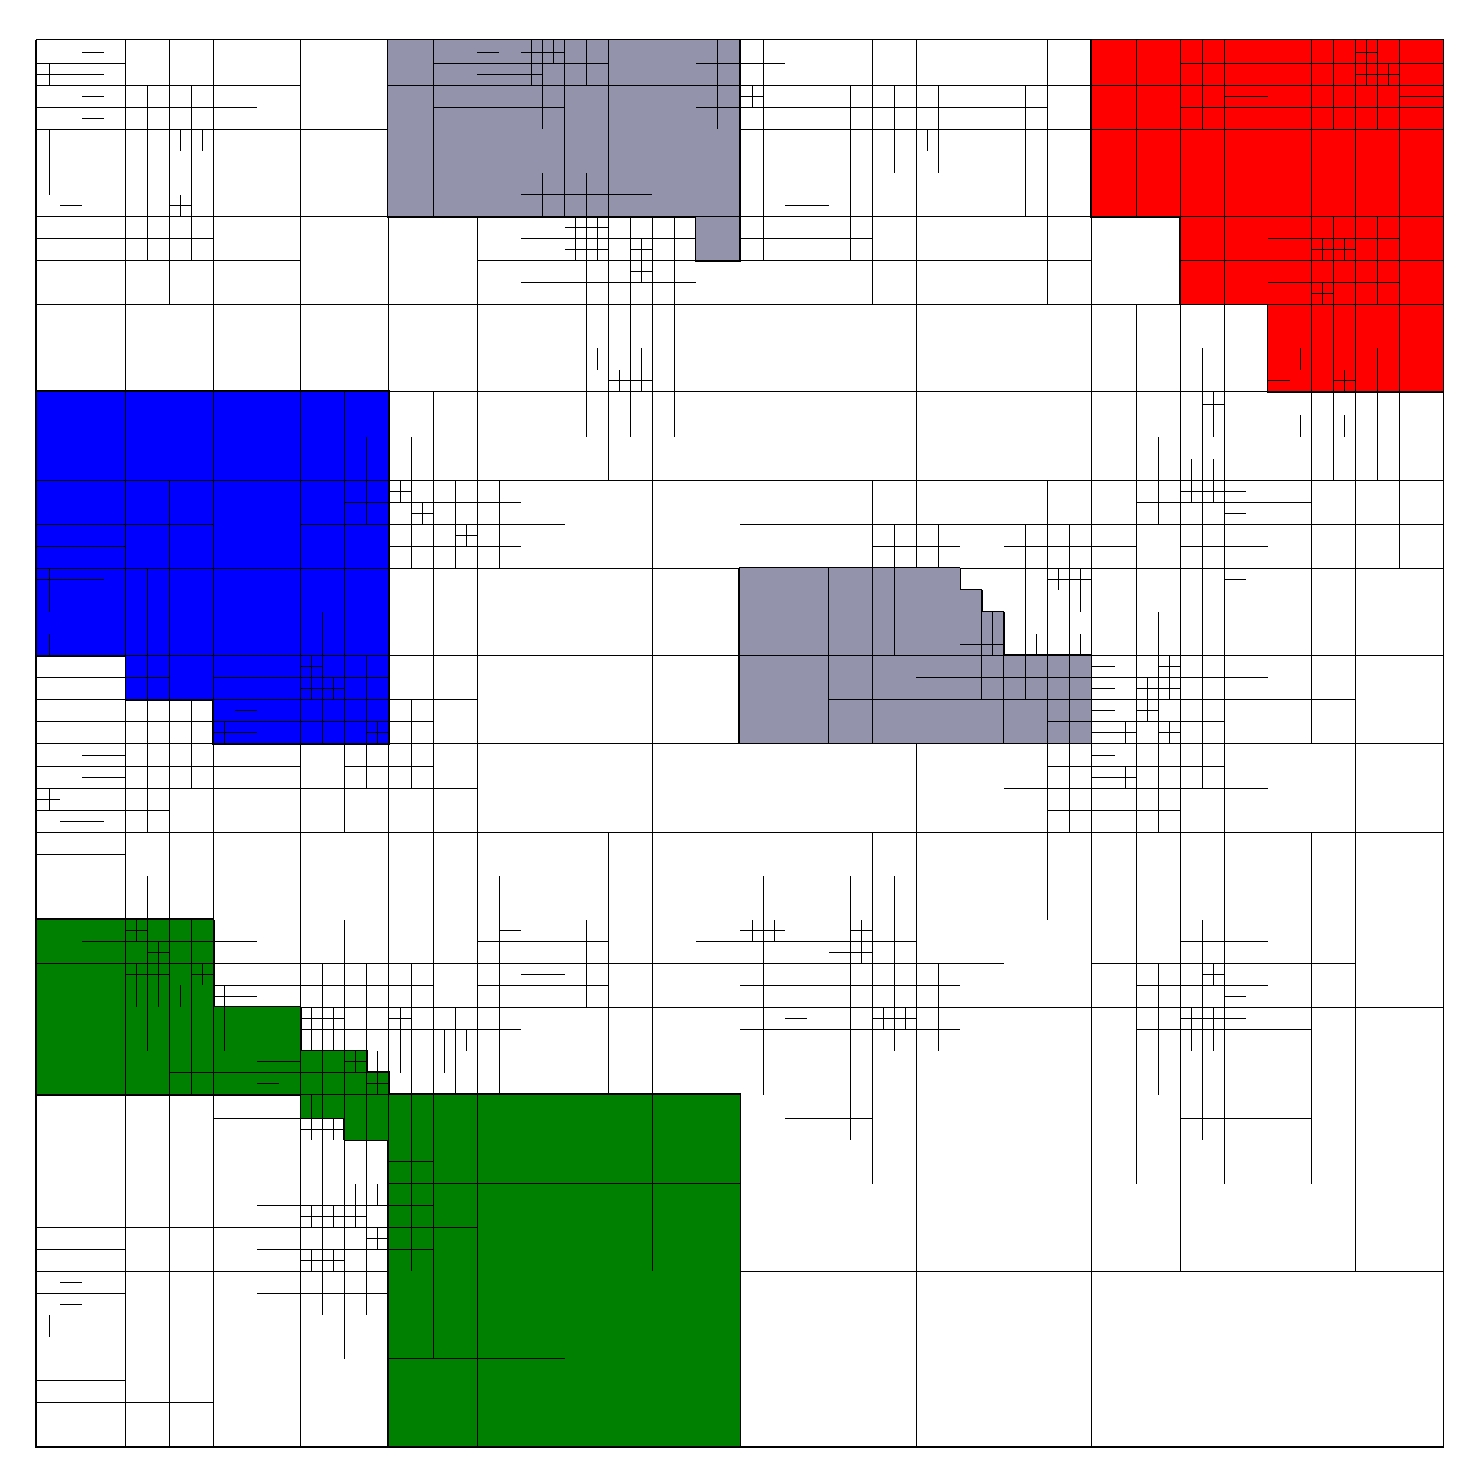
\includegraphics[width=0.45\textwidth]{Data/p4est_nonoverlapping.pdf}
    }
    \subfloat[Overlapping decomposition on which auxiliary operators $\{\mathring{A}_i\}_{i=1}^N$ are assembled.\label{fig:overlapping}]{
        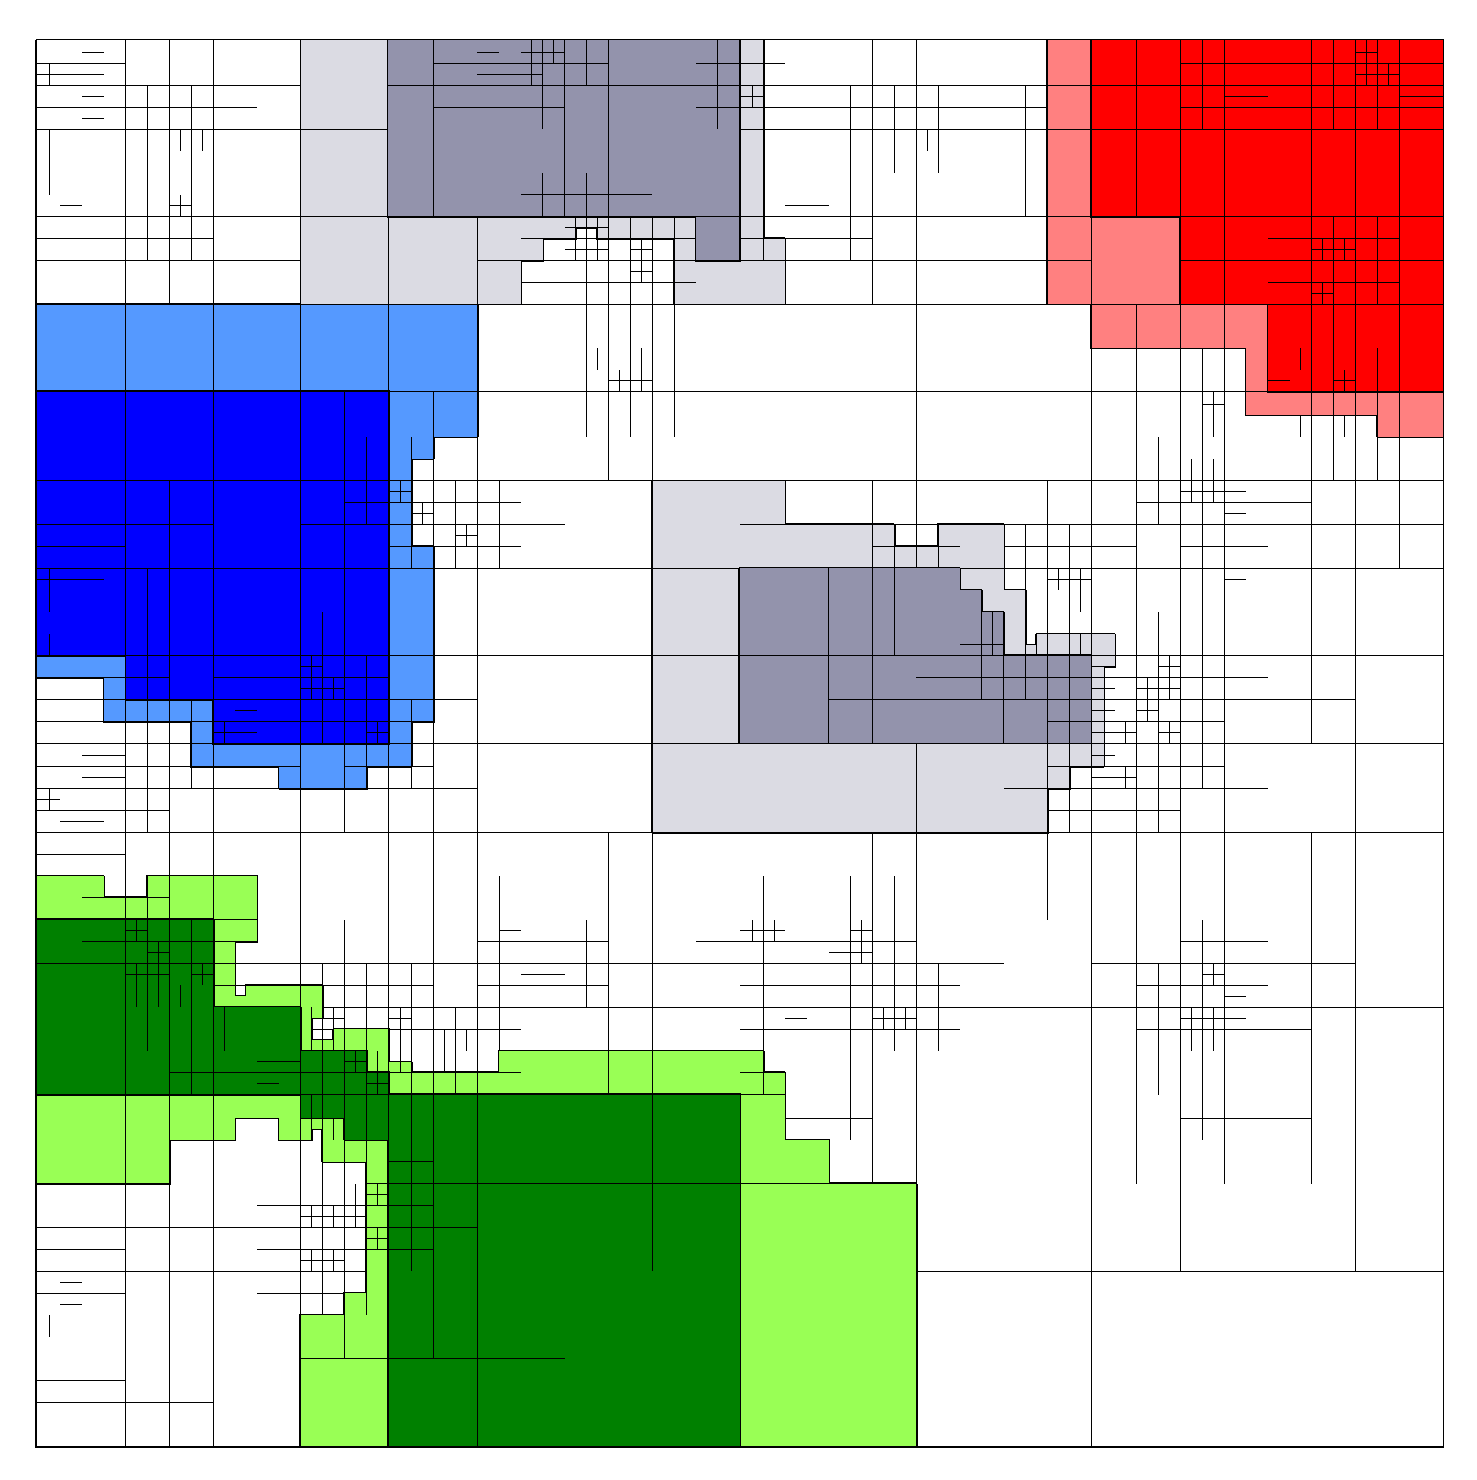
\includegraphics[width=0.45\textwidth]{Data/p4est_overlapping.pdf}
    }
    \caption{Automatic generation of overlapping subdomains when using a~\pk{DMPLEX}. For clarity, only four subdomains, one of which is disconnected, are colored.\label{fig:p4est}}
\end{figure}

With the local
matrix pencils available, new options will be automatically registered such as
\pk{-pc\_hpddm\_levels\_1\_eps\_nev} or \pk{-pc\_hpddm\_levels\_1\_eps\_threshold}, which
may be used to customize the eigenpairs SLEPc will compute in step \#2.  The
default \pk{-eps\_nev} value is 20, i.e., the dimension of the coarse space is
$20\times N$ under the assumption that all concurrent SLEPc solves converge.

For performance reasons, it is better to compute the same number of
eigenvectors on each process, since in this case the coarse operator will be
assembled using the \pk{MatMPISBAIJ} or \pk{MatMPIBAIJ} matrix type, with
usually large block sizes. This can have serious memory and performance
implications, see~\cref{fig:perfAX}. When applying the preconditioner,
\texttt{MPI\_Gather} and \texttt{MPI\_Scatter} operations are used to move
between levels, instead of the variable-size alternatives \texttt{MPI\_Gatherv}
and \texttt{MPI\_Scatterv}, that could exhibit worse performance. In addition,
standard eigensolvers such as \pk{EPSKRYLOVSCHUR} from SLEPc, cannot cheaply
evaluate the exact number of eigenpairs in a given interval of $\mathbb{R}^+$.
Instead, it is often more efficient to provide an upper bound of the number of
eigenpairs.

The option \pk{-pc\_hpddm\_coarse\_p} can be used to provide the size of the
subcommunicator that will be used to remap the coarse operator. With the default
value of 1, the coarse matrix $P^TAP$ is centralized on a single process.
The action of the inverses in~\cref{eq:two} can be parameterized through the
\pk{-pc\_hpddm\_coarse\_ksp\_type} and \pk{-pc\_hpddm\_levels\_1\_ksp\_type} options
respectively.

    \subsubsection{Coarse corrections customization}
Some other parameters may be adjusted to define how the one-level preconditioner
and the coarse grid operator interact. Besides the additive
correction shown in~\cref{eq:two}, end-users may select more numerically efficient
corrections~\cite{tang2009comparison,bastian1998additive} as:
\begin{align*}
    M'^{-1}_{\text{deflated}} &= Q + M^{-1}\left(I - AQ\right)\quad
    \text{(default)}\\
    M'^{-1}_{\text{balanced}} &= Q + \left(I - AQ\right)M^{-1}\left(I - AQ\right),
\end{align*}
with $Q = P \left(P^T A P\right)^{-1} P^T$ and $M^{-1}$ defined in~\cref{eq:one}. This is parameterized using the
options \pk{-pc\_hpddm\_coarse\_correction}
\pk{(deflated$|$additive$|$balanced)} or the routine
\pk{PCHPDDMSetCoarseCorrectionType}. It is important to keep in mind that all
these correction formulae may be applied to either a single vector or a block
of multiple vectors optimally. Indeed, the one-level preconditioner $M^{-1}$ is
applied with either \pk{PCApply} or \pk{PCMatApply}, and the
restriction-correction-interpolation operator $Q$ is applied in a block fashion
in HPDDM, and not column by column. See the effect of this strategy in~\cref{sec:lobpcg}.

    \subsubsection{Extension of the GenEO framework}
The local generalized eigenvalue problems~\cref{eq:gevp} can also be adjusted.
In addition to the local unassembled Neumann matrices~$\{\mathring{A}_i\}_{i=1}^N$,
users can prescribe additional local operators $\{B_i\}_{i=1}^N$, defined on
the overlapping decomposition, via the routine \pk{PCHPDDMSetRHSMat}(pc, $B_i$).
In the case of local matrices with optimized Robin transmission conditions, the
following generalized eigenvalue problems, called GenEO-2 in the
literature~\cite{haferssas2017soras}, are then solved in each subdomain:
\begin{equation*}
    \mathring{A}_i y_i = \lambda_i B_i y_i.
\end{equation*}
This may be useful when dealing with nearly indefinite systems, e.g., nearly
incompressible elasticity or the system of Stokes. Indeed, for such equations,
one needs to compute a lot of eigenvectors from the classical GenEO
eigenproblem~\cref{eq:gevp} to generate a robust preconditioner. GenEO-2
alleviates this phenomenon. In the case where the local operators
$\{B_i\}_{i=1}^N$ are the discrete mass matrices on the subdomains interfaces,
the so-called Dirichlet-to-Neumann coarse operator is constructed. This has
proven to be efficient for solving the heterogeneous Helmholtz
equation~\cite{conen2014coarse}.

    \subsubsection{Multilevel extension}\label{sec:ml}
In the previous sections, it was shown how to supply the required information to
\pk{PCHPDDM} in order to build robust two-level overlapping domain decomposition preconditioners.
Since the dimension of the
coarse operator linearly depends on the number of subdomains of the
fine level decomposition, switching to a multilevel scheme may alleviate the increasing cost
of solving the coarse linear system. A multilevel extension of the GenEO framework has been recently
proposed~\cite{aldaas2019multi}, with the advantage that the multilevel hierarchy can be
automatically constructed without any additional information from the user.

\pk{PCHPDDM} follows the same numbering of \pk{PCBDDC}:
the finest level is always numbered with 1, and the level index increases as the hierarchy is traversed, up until
the coarsest level, whose solver options are prefixed by \pk{coarse\_}. In order to
register an additional level $l' = l+1$, the following conditions must be met at
level $l$:
\begin{itemize}
    \item there must be more than one subdomain;
    \item at least one local eigenvector must be computed per coarse subdomain.
\end{itemize}
For example, using $N = 16$ subdomains on the finest level, the options

\pk{-pc\_hpddm\_levels\_1\_eps\_threshold 0.4 -pc\_hpddm\_coarse\_p 8}

\noindent will define a two-level method with the coarse operator being distributed
among 8 processes, assuming that there is globally enough $\lambda_i$ in~\cref{eq:gevp} smaller than the prescribed threshold 0.4.
Similarly, the options

\pk{-pc\_hpddm\_levels\_1\_eps\_nev 10 -pc\_hpddm\_levels\_2\_p 8}

\pk{-pc\_hpddm\_levels\_2\_eps\_nev 10 -pc\_hpddm\_coarse\_p 2}

\noindent will define
a three-level method with the second level distributed among 8 processes, while the coarsest level
will be built using 10 eigenvalues per subdomain from the second level and remapped onto 2 processes.
Additional examples for the solver customization are provided in~\cref{sec:pchpddm-examples}
%    \item \pk{-pc\_hpddm\_levels\_1\_eps\_nev 10 -pc\_hpddm\_levels\_2\_p 8} is not
%        valid because there are only two levels, so the options \pk{levels\_2\_} are
%        not registered and coarse\_ has to be used instead;
%    \item \pk{-pc\_hpddm\_levels\_1\_eps\_nev 10 -pc\_hpddm\_levels\_2\_eps\_nev 10} \linebreak \pk{-pc\_hpddm\_coarse\_p 2}
%        is not valid because there is no option \pk{levels\_2\_p}, so the default
%        value of 1 is used for the second level, and it is thus not possible to
%        define a third level with a single second-level subdomain.
%\end{itemize}

    \subsubsection{PCHPDDM for non-overlapping domain decomposition}
Because of the intrinsic nature of balancing domain
decomposition methods, \pk{PCNN} and \pk{PCBDDC} must be supplied a \pk{MatIS}
which stores local unassembled matrices and local to global mappings.
These local matrices are equivalent to the $\{\mathring{A}_i\}_{i=1}^N$
defined \cref{sec:interface-pc}, assuming the domain decomposition is without
overlap, see for example $\Omega_1$ and $\Omega_2$ from~\cref{fig:poisson} in a
finite element context. Since the assembled form of these operators can be reconstructed,
it is possible to get the Dirichlet operators
$\{R_i A R_i^T\}_{i=1}^N$ from~\cref{sec:interface-pc} as well. All tools needed by the
GenEO framework are thus readily available. Note however that one-level
overlapping Schwarz methods are known for converging slowly when there is in
fact no overlap. The proposed methodology is not strictly equivalent to the
BDD-GenEO method~\cite{spillane2013automatic}, in which local Schur complements
on subdomain interfaces are computed explicitly, and then used in concurrent
dense generalized eigenvalue problems.
%It is common in the field of BDD to see the coarse problem as
%an unassembled operator as well. In fact, this is mandatory to define efficient
%multilevel variants, as implemented in \pk{PCBDDC}. In~\cref{sec:bddc}, it will
%be shown how a coarse problem obtained in \pk{PCBDDC} may be solved using
%\pk{PCHPDDM}.
  \subsection{Applications and numerical results}\label{sec:pchpddm-examples}
    \subsubsection{System of elasticity}\label{sec:linear-elasticity}
We first report on solving the three-dimensional system of linear elasticity with highly heterogeneous elastic modulus.
Its strong formulation is given by:
\begin{align}
	\label{eq:elasticity}
	\begin{split}
		\text{div }\sigma (u)  + f	&= 0	\quad \text{in } \Omega,\\
		u														&= 0	\quad \text{on } \Gamma_D, \\
		\sigma (u) \cdot n					&= 0	\quad \text{on } \Gamma_N.
	\end{split}
\end{align}
The physical domain $\Omega$ is a beam of dimensions $[0,6] \times [0,1] \times [0,1]$.
The Cauchy stress tensor $\sigma$ is given by Hooke’s law: it can be expressed in terms of Young’s modulus $E$ and Poisson’s ratio $\nu$,
\[
	\sigma_{ij}(u) =
	\begin{cases}
		2\mu \varepsilon_{ij}(u)													\quad	& i \ne j, \\
		2\mu \varepsilon_{ii}(u) + \lambda \text{div}(u)	\quad	& i = j,
	\end{cases}
\]
where
\[
	\varepsilon_{ij}(u) = \frac{1}{2} \left(\frac{\partial u_i}{\partial x_i} + \frac{\partial u_j}{\partial x_j} \right), \mu = \frac{E}{2(1+\nu)}, \text{ and }\lambda = \frac{E\nu}{1-2\nu}.
\]
$\Gamma_D$ is the subset of the boundary of $\Omega$ corresponding to $x = 0$.
$\Gamma_N$ is defined as the complementary of $\Gamma_D$ with respect to the boundary of $\Omega$.
\Cref{eq:elasticity} is discretized using
$(\mathbb{P}_1, \mathbb{P}_1, \mathbb{P}_1)$ finite elements resulting in $\pgfmathprintnumber{593} \times 10^6$ number of unknowns
with approximately $\pgfmathprintnumber{45}$ nonzero coefficients per row.
The physical domain $\Omega$ is decomposed in $13{,}824$ subdomains using the automatic graph partitioner ParMETIS~\cite{karypis1998fast}.
There are heterogeneities due to jumps in $E$ and $\nu$. The following discontinuous piecewise constant values are considered: $(E_1, \nu_1) = ({\color{paraviewred}2\times 10^{11}}, 0.25)$ in blue regions, while $(E_2, \nu_2) = ({\color{paraviewblue}10^7}, 0.45)$ in red regions, see~\cref{fig:elas}.
The code used to produce these results was borrowed from
the original paper about the multilevel extension of
GenEO~\cite{aldaas2019multi} and it is available
at~\url{https://github.com/prj-/aldaas2019multi}.
\begin{figure}[htbp]
  \centering
  \begin{tikzpicture}[remember picture]
      \node[inner sep=-0.1cm] (fig) {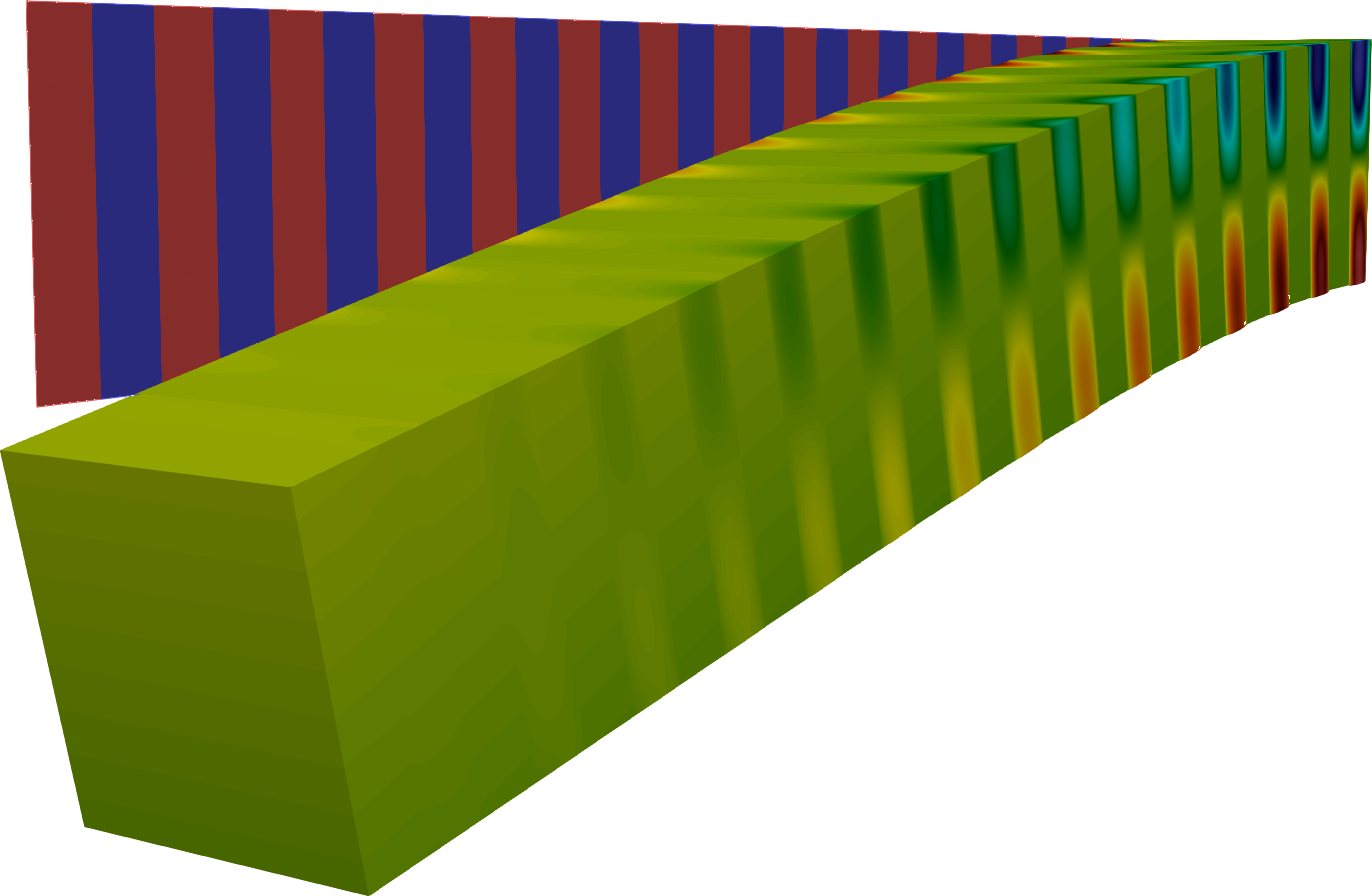
\includegraphics[width=0.55\textwidth]{Data/elasticity.png}};
  \end{tikzpicture}
      \begin{tikzpicture}[overlay,remember picture]
      \begin{axis}[
              at=(fig.south west),
          xshift=-2.25cm,yshift=-2cm,
    enlargelimits=false,
    colorbar,
    colormap name=paraview,
    point meta min=-4.9e-3,
    point meta max=4.9e-3,
    hide axis,
    colorbar style={
        ytick style={draw=none},
          title={$u(x, \cdot, z)$},
        scaled y ticks = false,
        height = 2.0cm,
        font = \tiny,
        width = 0.3cm,
        ytick={-4.9e-3,0.0,4.9e-3}
    }
    ]
      \end{axis}
  \end{tikzpicture}
    \caption{Deformed geometrical configuration of a 3D clamped beam subject to gravity. The striped plane in the background shows a cut of the resting configuration with the jumps in the coefficient $E_1={\color{paraviewblue}10^7}$ and $E_2={\color{paraviewred}2\times 10^{11}}$, aligned with those of $\nu$.\label{fig:elas}}
\end{figure} \\
The following preconditioners are compared:
\begin{enumerate}
    \item \pk{PCGAMG};\label{enum:gamg}
    \item \pk{PCHPDDM} with an exact coarse solver;\label{enum:exact}
    \item \pk{PCHPDDM} with inexact coarse solvers using GenEO multilevel extension.\label{enum:inexact} %, cf.~\cref{sec:ml}.\label{enum:inexact}
\end{enumerate}
The flexible GMRES is used and customized with the options \pk{-ksp\_gmres\_modifiedgramschmidt
-ksp\_gmres\_restart 50
-ksp\_type fgmres}. The options specific to each solver described above are given below. \\[-4pt]
\begin{minipage}[t]{0.34\textwidth}
\begin{Verbatim}[fontsize=\footnotesize,frame=single,framerule=0.1mm,commandchars=\\\{\}]
\fvtextcolor{mygreen}{# cf. \cref{enum:gamg}}
-pc_type gamg
-prefix_push pc_gamg_
 -threshold 0.03
 -square_graph 4
 -sym_graph true
 -asm_use_agg true
 -repartition true
-prefix_pop
-prefix_push mg_levels_
 -pc_asm_overlap 0
 -sub_pc_type cholesky
-prefix_pop
-prefix_push mg_coarse_
 -pc_type redundant
 -redundant_pc_type cholesky
-prefix_pop
\end{Verbatim}
\end{minipage}
\hfill
\begin{minipage}[t]{0.49\textwidth}
\begin{Verbatim}[fontsize=\footnotesize,frame=single,framerule=0.1mm,commandchars=\\\{\}]
\fvtextcolor{mygreen}{# cf. \cref{enum:exact}}
-pc_type hpddm
-prefix_push pc_hpddm_
 -prefix_push levels_1_
  -pc_type     asm
  -eps_nev     40
  -sub_pc_type cholesky
  -sub_pc_factor_mat_solver_type mumps
  -st_pc_factor_mat_solver_type mumps
 -prefix_pop
 -prefix_push coarse_
  -p 24
  -pc_factor_mat_solver_type mkl_cpardiso
 -prefix_pop
 -define_subdomains
 -has_neumann
-prefix_pop
\end{Verbatim}
\end{minipage} \\
By default, the coarse problem in \pk{PCHPDDM} is solved using an exact $LU$ or Cholesky factorization, in this case using 24 processes and MKL CPARDISO. Switching to an inexact solver using the multilevel extension of GenEO, cf.~\cref{enum:inexact}, is straightforward. \\[-4pt]
\begin{minipage}[t]{0.525\textwidth}
\begin{Verbatim}[fontsize=\footnotesize,frame=single,framerule=0.1mm,commandchars=\\\{\}, codes={\catcode`$=3\catcode`^=7}]
\fvtextcolor{mygreen}{# cf. \cref{enum:inexact}}
-prefix_push pc_hpddm_levels_2_
 -p           $M$
 -ksp_type    gmres
 -ksp_rtol    1.0e-2
 -ksp_pc_side right
 -pc_type     asm
 -eps_nev     80
 -sub_pc_type cholesky
 -sub_pc_factor_mat_solver_type mkl_pardiso
 -st_pc_factor_mat_solver_type mkl_pardiso
-prefix_pop
\end{Verbatim}
\end{minipage} \\
In this third configuration, $M$ is the number of subdomains used to define the second-level domain decomposition, which is an aggregation of first-level subdomains.

Considering the parametrization used for the \pk{PCHPDDM} solvers, \cref{enum:exact} and \cref{enum:inexact} yield the same number of outer iterates. In~\cref{fig:gamg-geneo}, the convergence history of \pk{PCGAMG} and \pk{PCHPDDM} are reported. In~\cref{fig:inexact}, the number of inner coarse iterations are reported for various values of $M$. In the case of a two-level method,~\cref{enum:exact}, this number is equal to one and is thus not reported in the figure.
\pgfplotstableread{
    it gamg hpddm
  0 3.859411178402e+00 3.859411178402e+00
  1 3.859411159689e+00 3.859411176864e+00
  2 3.859410249427e+00 3.859411160502e+00
  3 3.859409408276e+00 3.859411009079e+00
  4 3.859405618616e+00 3.859410641267e+00
  5 3.859384473758e+00 3.859409504108e+00
  6 3.859336132196e+00 3.859406284759e+00
  7 3.859180574117e+00 3.859396774066e+00
  8 3.858527456325e+00 3.859371139173e+00
  9 3.855946156750e+00 3.859291203708e+00
 10 3.847882304613e+00 3.859050327998e+00
 11 3.823783202371e+00 3.858349404873e+00
 12 3.761793608189e+00 3.856196410336e+00
 13 3.604276380304e+00 3.850223368267e+00
 14 3.219169630144e+00 3.833574948206e+00
 15 2.524138668209e+00 3.789137446493e+00
 16 1.612332237539e+00 3.677085304126e+00
 17 9.250281017522e-01 3.416685094366e+00
 18 5.244208314872e-01 2.914257430799e+00
 19 2.900205723223e-01 2.201797784976e+00
 20 1.639686082701e-01 1.504764597680e+00
 21 8.999329395027e-02 9.651409800649e-01
 22 4.806932060093e-02 5.991352736022e-01
 23 2.623490189992e-02 3.709375100943e-01
 24 1.420399852677e-02 2.262545029178e-01
 25 7.785203261213e-03 1.386897546734e-01
 26 4.279336819903e-03 8.468744514883e-02
 27 2.392528915920e-03 5.199440557582e-02
 28 1.398509701362e-03 3.167797843106e-02
 29 7.951946917375e-04 1.958093540992e-02
 30 4.302913355532e-04 1.195194560026e-02
 31 2.336327784594e-04 7.371078209494e-03
 32 1.242918661343e-04 4.565136636812e-03
 33 6.466088102124e-05 2.757997749188e-03
 34 3.347704352999e-05 1.722488935062e-03
 35               nan  1.040719253466e-03
 36               nan  6.471646548950e-04
 37               nan  3.944692230299e-04
 38               nan  2.413209464780e-04
 39               nan  1.481390561258e-04
 40               nan  9.041135719421e-05
 41               nan  5.606739576810e-05
 42               nan  3.445256788047e-05
}\comparisontable
\pgfplotstableread{
it p-16  p-256  p-1024
 1 26    16     13
 2 9     6      6
 3 10    7      6
 4 8     6      6
 5 9     6      5
 6 5     5      5
 7 8     6      5
 8 9     6      5
 9 7     5      5
10 7     6      5
11 7     6      5
12 8     6      5
13 5     5      5
14 6     6      4
15 6     5      5
16 8     6      5
17 6     5      5
18 6     5      5
19 7     5      4
20 8     6      5
21 8     6      5
22 7     5      4
23 7     6      5
24 6     6      5
25 6     6      5
26 6     5      5
27 6     5      4
28 5     5      5
29 6     5      5
30 6     5      5
31 7     5      5
32 8     6      5
33 7     6      4
34 5     5      5
35 5     5      5
36 6     5      4
37 6     5      4
38 6     5      5
39 7     5      4
40 5     5      5
41 5     5      5
42 6     5      nan
43 5     nan    nan
}\comparisonP
\begin{figure}[htbp]
  \centering
    \subfloat[\parbox{5cm}{Numerical comparison of \pk{PCGAMG} and \pk{PCHPDDM}.\label{fig:gamg-geneo}}]{
\begin{tikzpicture}[font=\scriptsize]
\begin{semilogyaxis}[xmin=0,xmax=50,width=0.46\textwidth,
    ymajorgrids,
    xlabel={Iteration number},
    ylabel={Unpreconditioned residual},
    enlarge x limits=0.05,
% yticklabel={
% \pgfmathparse{int(\tick)}
% \ifnum\pgfmathresult=0
% $1$
% \else
% \pgfmathparse{int(\tick/ln(10))}{$10^{\pgfmathresult}$}
% \fi
% }
]
\addplot[very thick,last] table [x=it, y index=1] {\comparisontable};
\addplot[very thick,myred, densely dashed] table [x=it, y index=2]       {\comparisontable};
    \legend{{\pk{PCGAMG}},{\pk{PCHPDDM}}}
% lightgray
\end{semilogyaxis}
\end{tikzpicture}
}
    \subfloat[\parbox{5cm}{\# of inner coarse iterations for various values of $M$, the number of second-level subdomains.}\label{fig:inexact}]{
        \begin{tikzpicture}[font=\scriptsize]
\begin{axis}[%title=\framebox{{\upcase diffusion 2D, $\mathbb{P}_4$ FE, $\varepsilon = \num[exponent-product=\cdot]{1e-06}$}},
        ymajorgrids, unbounded coords=jump, xmin=-1,extra y ticks={100}, width=0.46\textwidth,extra y tick labels=\empty, extra y tick style={grid=major},legend columns=3,legend cell align=left, ylabel = {\# of inner iterations}, xlabel = {Outer iteration index}]
\addlegendimage{empty legend}
\addlegendimage{empty legend}
\addlegendimage{empty legend}
\addplot[last, very thick] table[x=it, y=p-16] {\comparisonP};\label{pgfplots:p-16}
\addplot[myred, densely dashed, very thick] table[x=it, y=p-256] {\comparisonP};\label{pgfplots:p-256}
\addplot[myyellow, densely dotted, very thick] table[x=it, y=p-1024] {\comparisonP};\label{pgfplots:p-1024}

   \addlegendentry{\hspace{-.6cm}-pc\_hpddm\_levels\_2\_p $M$ \hspace*{-2.5cm}}
   \addlegendentry{}
   \addlegendentry{}
   \addlegendentry{16}
   \addlegendentry{256}
    \addlegendentry{\pgfmathprintnumber{1024}}
\end{axis}
        \end{tikzpicture}
    }
    \caption{Convergence histories of \pk{PCGAMG} and \pk{PCHPDDM} for solving the 3D system of linear elasticity. For \pk{PCHPDDM}, a comparison of the number of inner coarse iterations is displayed when using an inexact method, cf.~\cref{enum:inexact}.}
\end{figure}
Note that in this test case, \pk{PCGAMG} is faster than all \pk{PCHPDDM}
alternatives. For \pk{PCGAMG}, the setup phase takes 70 seconds, while the solution phase requires 19 seconds;
on the other hand, the fastest \pk{PCHPDDM} configuration, which corresponds to
configuration~\ref{pgfplots:p-256} with 256 second-level subdomains, requires 64 seconds to setup and 31 for the solution of the linear system.
Out of the 64 seconds needed for \pk{PCHPDDM} setup, 31 are spent in SLEPc
\pk{EPSSolve} for solving GenEO at each level but the coarsest. With respect to
coarsening, \pk{PCGAMG} has an operator complexity of 1.501, while for \pk{PCHPDDM},
it is 1.015.
    \subsubsection{Liouville--Bratu--Gelfand equation} The strong formulation of this nonlinear problem is given by:
\begin{equation}
    -\nabla \cdot (\kappa \nabla u) - 6.2 \exp^u = 0,\label{eq:bratu}
\end{equation}
where $\kappa$ is a heterogeneous coefficient distribution,
see~\cref{fig:kappa}. This equation may model the temperature distribution in
combustion models. Here, it is merely used to test \pk{PCHPDDM} in the context
of solving successive linearized equations%, but there are many other techniques for solving such a nonlinear equation, such as first decomposing the domain and then linearizing the equation~\cite{dryja1997nonlinear}
. The physical domain $\Omega$ is the unit cube. It is decomposed in $10{,}272$ subdomains.
\Cref{eq:bratu} is discretized using $\mathbb{P}_2$ finite elements.
The number of unknowns is $\pgfmathprintnumber{217} \times 10^6$, with
approximately $\pgfmathprintnumber{29}$ nonzero coefficients per row.
It is solved using a \pk{SNES}, with \pk{PCHPDDM} being the preconditioner for
solving each linearized system, see~\cref{fig:u}.
\begin{figure}[htbp]
  \centering
  \subfloat[Coefficient distribution.\label{fig:kappa}]{
  \begin{tikzpicture}[remember picture]
      \node[inner sep=-0.1cm] (fig) {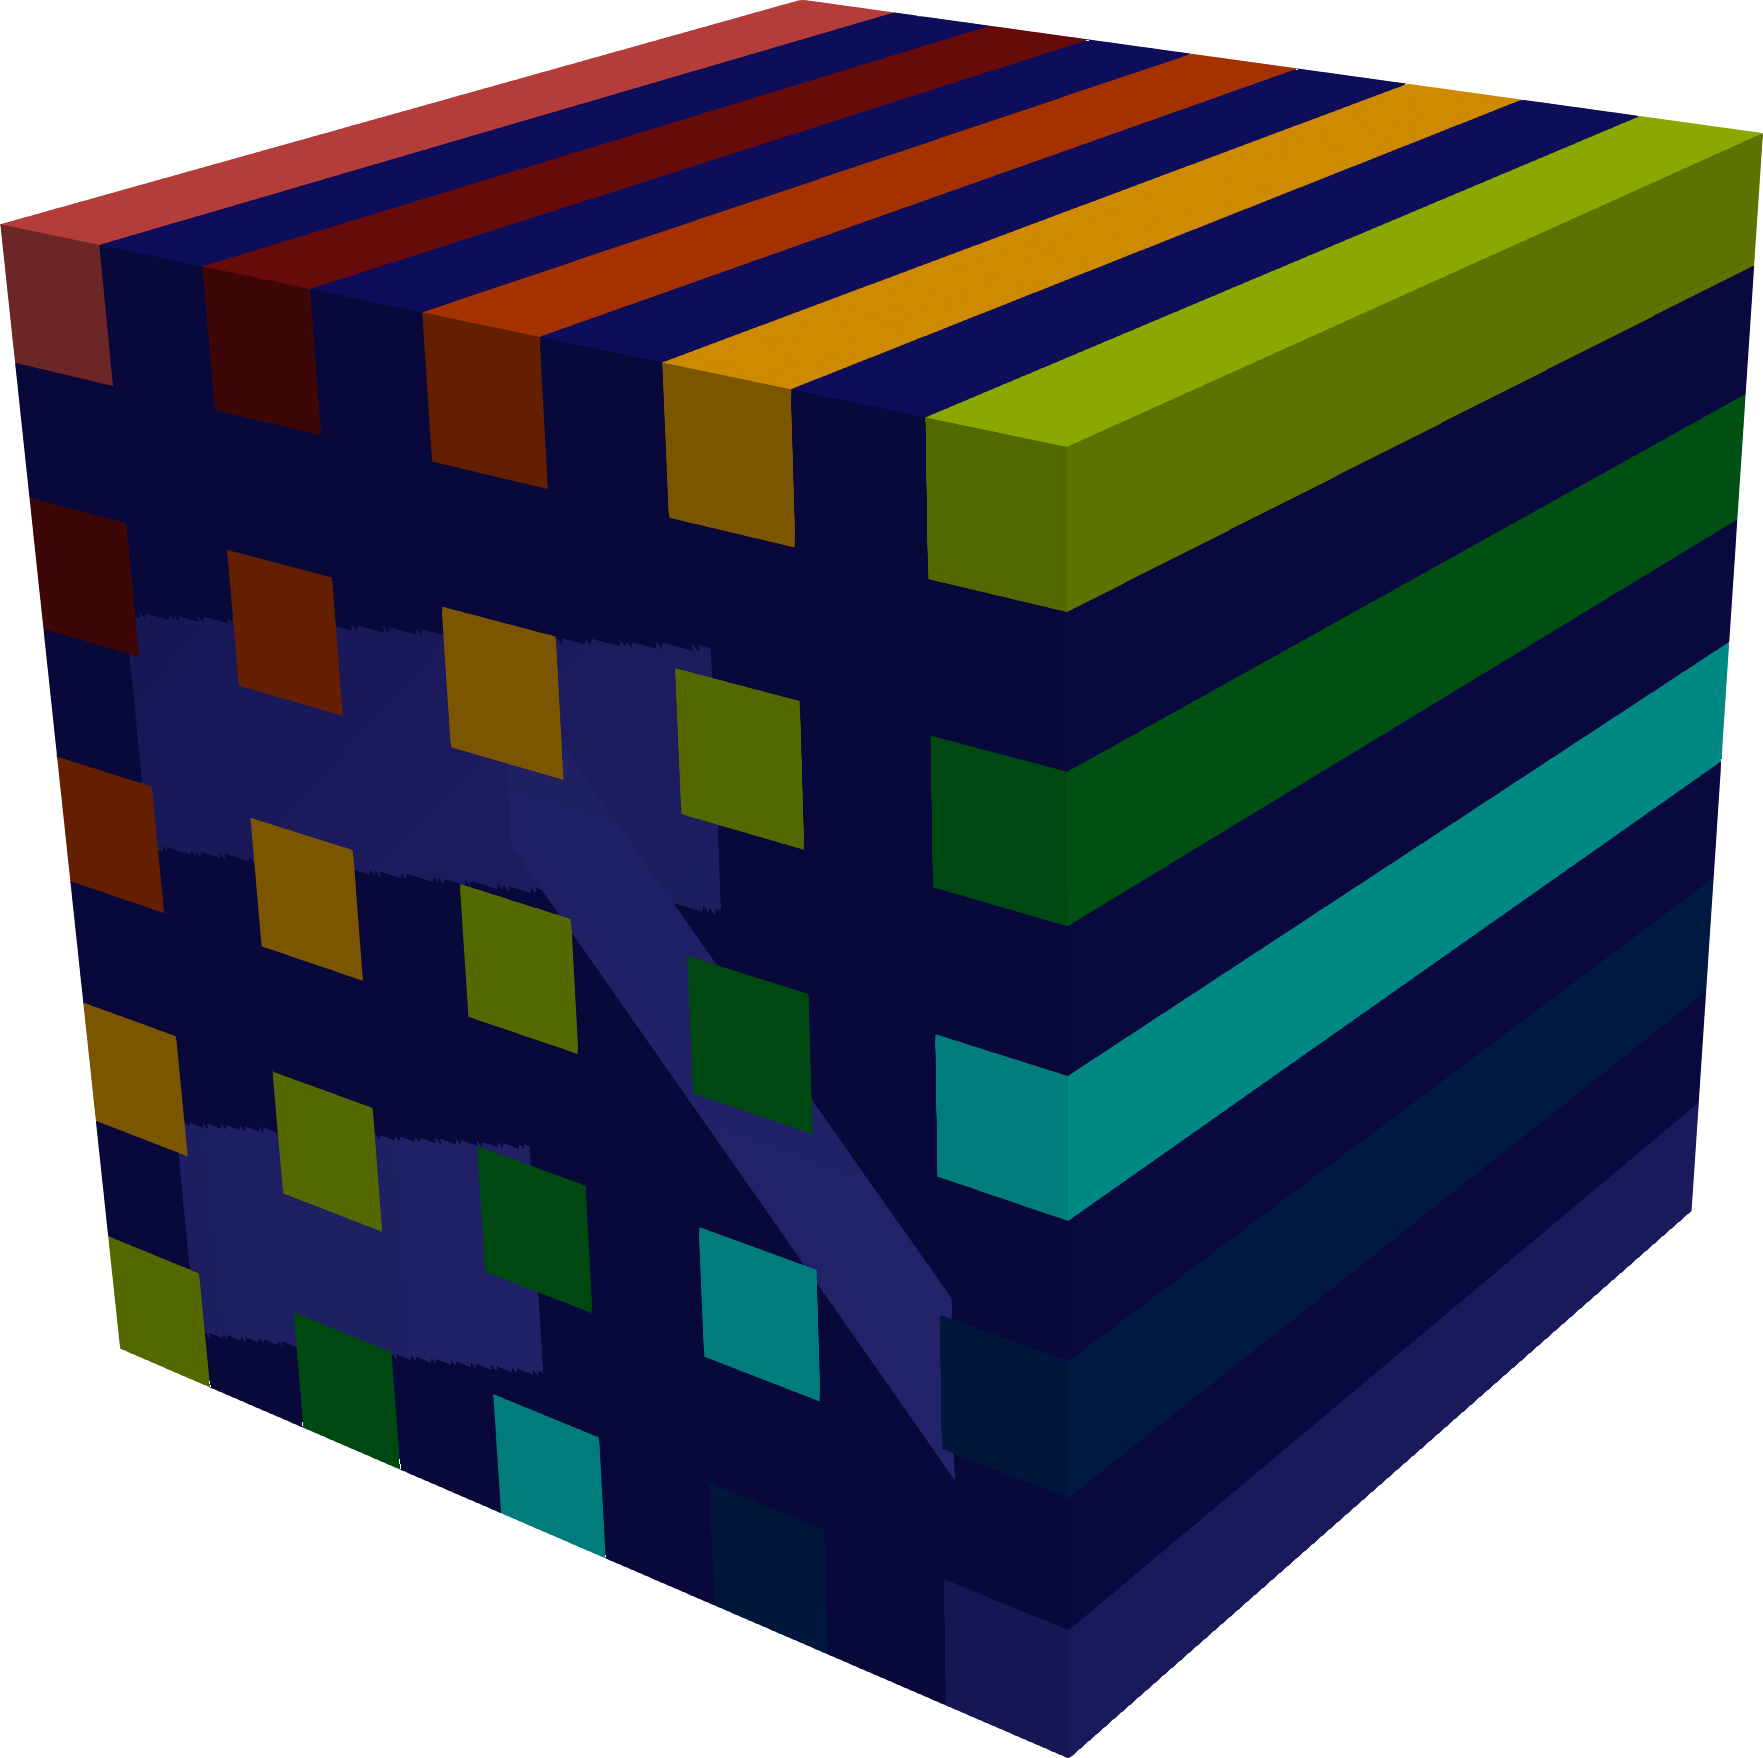
\includegraphics[width=0.45\textwidth]{Data/kappa.png}};
  \end{tikzpicture}
  }
    \subfloat[Isosurfaces of the solution.\label{fig:u}]{
  \begin{tikzpicture}[remember picture]
      \node[inner sep=-0.1cm] (fq) {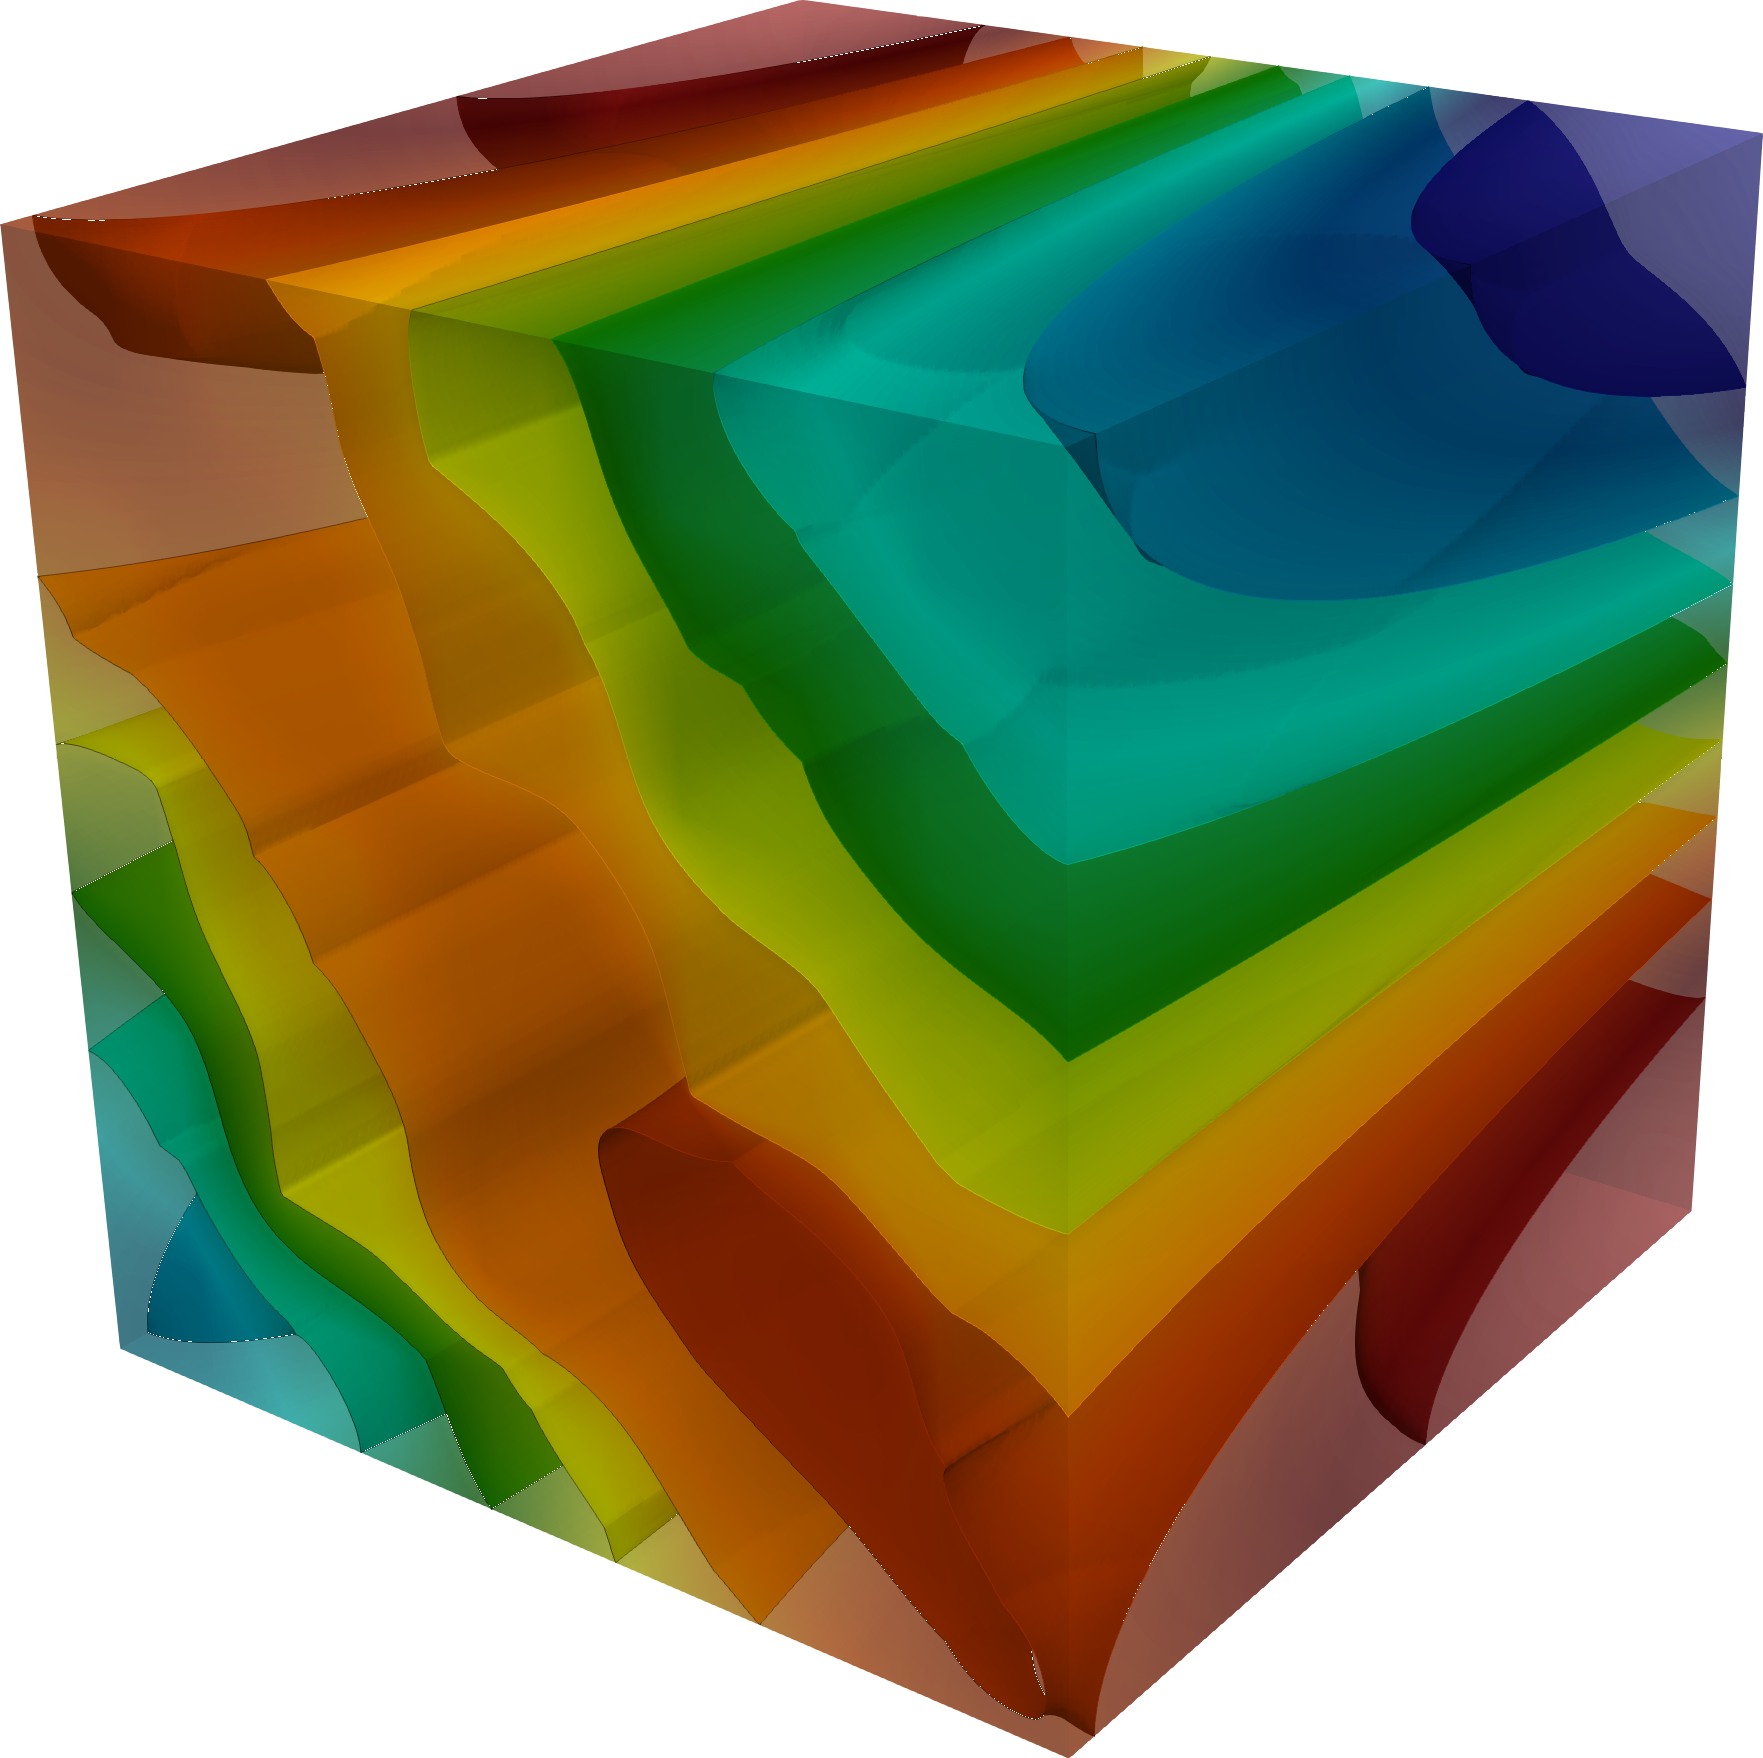
\includegraphics[width=0.45\textwidth]{Data/u.png}};
  \end{tikzpicture}
      \begin{tikzpicture}[overlay,remember picture]
      \begin{axis}[
              at=(fig.south west),
          xshift=-1.5cm,yshift=-2cm,
    enlargelimits=false,
    colorbar,
    colormap name=paraview,
    point meta min=6e-2,
    point meta max=8.5,
    hide axis,
    colorbar style={
        ytick style={draw=none},
        title={$\kappa$},
        scaled y ticks = false,
        height = 2.0cm,
        font = \tiny,
        width = 0.3cm,
        ytick={6e-2,4.0,8.5}
    }
    ]
      \end{axis}
      \begin{axis}[
              at=(fq.south east),
          xshift=0.0cm,yshift=-2cm,
    enlargelimits=false,
    colorbar,
    colormap name=paraview,
    point meta min=-1.9,
    point meta max=1.9,
    hide axis,
    colorbar style={
        ytick style={draw=none},
        title={$u$},
        scaled y ticks = false,
        height = 2.0cm,
        font = \tiny,
        width = 0.3cm,
        ytick={-1.9,0,1.9}
    }
    ]
      \end{axis}
  \end{tikzpicture}
  }
    \caption{Solving the Liouville--Bratu--Gelfand equation using \pk{SNESNEWTONLS} and \pk{PCHPDDM}.}
\end{figure}
The GenEO framework has seldom been used in the context of nonlinear problems, but
here, it is shown that it can solve the linearized equations
from~\cref{eq:bratu} in few iterates.  There are two strategies to define the
\pk{PC} here:
\begin{itemize}
\item whenever the Jacobian is being updated in the \pk{SNESSetJacobian}
function, new unassembled Neumann matrices at the current linearization point are updated as well and supplied to the previously
explained \pk{PCHPDDMSetAuxiliaryMat} function, this is done automatically if the nonlinear solver is attached to a
\pk{DMPLEX} or a \pk{DMP4EST};
\item by reusing the \pk{PCHPDDM} hierarchy assembled when solving the first
    linearized system, using the \pk{SNESSetLagPreconditioner} option.
\end{itemize}
Since the system is not too stiff here, both strategies lead to the same
convergence history, which is displayed in~\cref{fig:bratu-conv}. The complete set of
options is given in~\cref{fig:bratu-options}. Results can be reproduced using the FreeFEM script at \url{https://github.com/prj-/jolivet2020petsc}
\pgfplotstableread{
it first                second               third                  fourth
 0 1.199398376742e+01   3.397386070782e-04   1.863266214507e-05     8.796157053238e-07
 1 3.105058690048e+00   3.396971540287e-04   1.863121679230e-05     8.795510768269e-07
 2 7.493003609951e-01   3.394715205399e-04   1.862509132651e-05     8.792972699303e-07
 3 2.066956200353e-01   3.372614259474e-04   1.860041089031e-05     8.783878285049e-07
 4 6.309969159499e-02   3.127230257133e-04   1.838790479520e-05     8.701902993653e-07
 5 1.933161037163e-02   2.148249088439e-04   1.707968608004e-05     8.181649294279e-07
 6 6.550219066971e-03   9.681223676375e-05   1.238892191333e-05     6.183954841666e-07
 7 2.324009861121e-03   3.933958932173e-05   6.179174147298e-06     3.194732043996e-07
 8 8.476764474277e-04   1.558086376310e-05   2.605805785728e-06     1.363806062938e-07
 9 3.138242119678e-04   6.269961516841e-06   1.052999054933e-06     5.522010168719e-08
10 1.183695049547e-04   2.522978646378e-06   4.300851965899e-07     2.257459993685e-08
11                nan   1.024961124607e-06   1.753694476531e-07     9.219016303441e-09
12                nan   4.249085515277e-07   7.338448965970e-08     3.852685693794e-09
13                nan   1.763394120011e-07   3.059024771687e-08     1.609255024084e-09
14                nan   7.432342714299e-08   1.297122798875e-08     6.817901759942e-10
15                nan   3.135242203325e-08   5.496143820621e-09     2.896018108835e-10
16                nan   1.326698994886e-08   2.331975304171e-09     1.226613149417e-10
17                nan   5.639489438404e-09   9.871150757910e-10     5.194784893432e-11
18                nan   2.342602656325e-09   4.069402853378e-10     2.137940700304e-11
19                nan                  nan   1.679412238393e-10     8.828401758238e-12
20                nan                  nan                  nan     3.628457807677e-12
}\comparisonBratu
% 4 SNES Function norm 2.502417058684e-09
\begin{SaveVerbatim}[commandchars=\\\{\}]{VerbEnv}
-snes_type            newtonls
-snes_linesearch_type basic
-ksp_pc_side          right
-pc_type              hpddm
-prefix_push pc_hpddm_
 -prefix_push levels_1_
  -pc_type     asm
  -eps_nev     10
  -sub_pc_type cholesky
  -sub_pc_factor_mat_solver_type mumps
 -prefix_pop
 -coarse_p 128
 -define_subdomains
 -has_neumann
-prefix_pop
\end{SaveVerbatim}
\begin{figure}[htbp]
  \centering
    \subfloat[Convergence histories of the four linearized systems.
    At the top of each curve, for the first iterate, the value of the function
    norm is displayed.\label{fig:bratu-conv}]{
\begin{tikzpicture}[font=\scriptsize]
\begin{semilogyaxis}[clip=false,xmin=0,xmax=68,width=0.49\textwidth,
    legend style={at={(1.05,0.95)},cells={anchor=west}},ymajorgrids,
    xlabel={Iteration number},
    extra x ticks={0, 10, 28, 47, 67},extra x tick labels=\empty,
    extra x tick style={grid=major},
    ylabel={Relative unpreconditioned residual},
    enlarge x limits=0.05,
yticklabel={
\pgfmathparse{int(\tick)}
\ifnum\pgfmathresult=0
$1$
\else
\pgfmathparse{int(\tick/ln(10))}{$10^{\pgfmathresult}$}
\fi
}
]
\addplot[very thick,last] table [x=it, y expr=\thisrowno{1}/1.199398376742e+01] {\comparisonBratu};
\addplot[very thick,last] table [x expr=\thisrowno{0}+10, y expr=\thisrowno{2}/3.397386070782e-04] {\comparisonBratu};
\addplot[very thick,last] table [x expr=\thisrowno{0}+28, y expr=\thisrowno{3}/1.863266214507e-05] {\comparisonBratu};
\addplot[very thick,last] table [x expr=\thisrowno{0}+47, y expr=\thisrowno{4}/8.796157053238e-07] {\comparisonBratu};
\node[font=\tiny,fill=white,inner sep=1pt] at (axis cs:0, 2) {12.0};
\node[font=\tiny,fill=white,inner sep=1pt] at (axis cs:12, 2) {3.4E-4};
\node[font=\tiny,fill=white,inner sep=1pt] at (axis cs:28, 2) {1.9E-5};
\node[font=\tiny,fill=white,inner sep=1pt] at (axis cs:47, 2) {8.8E-7};
\node[font=\tiny,fill=white,inner sep=1pt] at (axis cs:67, 2) {2.5E-9};
\end{semilogyaxis}
\end{tikzpicture}
}
    \subfloat[\parbox{5cm}{\pk{SNES}, \pk{KSP}, and \pk{PC} options for
    solving~\cref{eq:bratu}}\label{fig:bratu-options}]{
        {\setlength{\fboxrule}{0.1mm}
        \fbox{\BUseVerbatim[fontsize=\footnotesize]{VerbEnv}}
        }
    }
    \caption{Numerical performance of \pk{PCHPDDM} in a nonlinear context for
    solving the Liouville--Bratu--Gelfand equation. Default PETSc tolerances are used:
    $10^{-5}$ decrease of relative residuals for linear solves, $10^{-8}$ decrease
    of function norms for nonlinear solves.}
\end{figure}
    \subsubsection{Using PCHPDDM as a coarse grid solver for PCBDDC\label{sec:bddc}}
A last toy problem is here proposed to show how one may switch between a multilevel
BDDC solver to a two-level BDDC solver using \pk{PCHPDDM} for solving the
coarse problem. The problem is generated using MFEM~\cite{anderson2019mfem}
definite Maxwell example available at \url{https://github.com/mfem/mfem/blob/master/examples/petsc/ex3p.cpp}.
The strong formulation of the continuous problem is given by:
\begin{align}
	\label{eq:maxwell}
	\begin{split}
        \nabla \times (\nabla \times E) + E	&= 0	\quad \text{in } \Omega,\\
        E \times n					&= (1+16\pi^2)\begin{bmatrix} \sin{4\pi y}&
        \sin{4\pi z}&\sin{4\pi x} \end{bmatrix}^T \text{on } \partial \Omega.
	\end{split}
\end{align}
It is discretized using first order N\'ed\'elec finite elements and \pk{PCBDDC}
is automatically customized to obtain a stable method with these
elements~\cite{zampini2017balancing}. The number of unknowns is $\pgfmathprintnumber{5.6} \times 10^6$.
The following command line options are used. \\[-4pt]
\begin{Verbatim}[fontsize=\footnotesize,frame=single,framerule=0.1mm,commandchars=&\[\]]
&fvtextcolor[mygreen][$] &fvtextcolor[myyellow][mpirun] -n 512 ./ex3p -m ../../data/fichera.mesh -f 4 --petscopts rc_ex3p_bddc      &fvtextcolor[myred][\]
  --nonoverlapping
\end{Verbatim}
The option file shows how \pk{PCHPDDM} may be composed into \pk{PCBDDC}. \\[-4pt]
\begin{minipage}[t]{0.565\textwidth}
\begin{Verbatim}[fontsize=\footnotesize,frame=single,framerule=0.1mm,commandchars=&\[\]]
&fvtextcolor[mygreen][$] &fvtextcolor[myyellow][cat] rc_ex3p_bddc
-ksp_type      fgmres
-ksp_norm_type unpreconditioned
-ksp_rtol      1.0e-8

-prefix_push pc_bddc_
 -use_deluxe_scaling
 -levels             1
 -adaptive_threshold 2.0
 -coarsening_ratio   8

 -neumann_pc_factor_mat_solver_type   mumps
 -dirichlet_pc_factor_mat_solver_type mumps
&fvtextcolor[mygreen][# continue on the right column]
\end{Verbatim}
\end{minipage}
\begin{minipage}[t]{0.425\textwidth}
\begin{Verbatim}[fontsize=\footnotesize,frame=single,framerule=0.1mm,commandchars=&\[\]]
&fvtextcolor[mygreen][# continued from the left column]
 -prefix_push coarse_
  -ksp_converged_reason
  -ksp_type      gmres
  -ksp_max_it    100
  -ksp_rtol      1.0e-1
  -pc_type       hpddm
  -ksp_norm_type preconditioned
  -prefix_push pc_hpddm_
   -levels_1_pc_type     asm
   -levels_1_eps_nev     10
   -levels_1_sub_pc_type cholesky
   -coarse_pc_type       cholesky
  -prefix_pop
 -prefix_pop
-prefix_pop
\end{Verbatim}
\end{minipage}
Deluxe scaling is used to build an adaptive second level with \pk{PCBDDC}. On this
second level with 16${,}$284 unknowns, new subdomains are built by aggregating the coarse element matrices of
8 fine-level subdomains. The BDDC coarse problem composed of $\frac{512}{8} =
64$ subdomains is then solved using \pk{PCHPDDM}, which itself builds another adaptive
level using $10$ local eigenvectors per subdomain. The coarsest level is
aggregated on a single process and solved using an exact Cholesky factorization.
The magnitude of the electric field is plotted in~\cref{fig:E}. The
convergence history of the solver is shown in~\cref{fig:BDDC}. The outer solver
reaches the prescribed convergence tolerance in 17 iterations~\ref{pgfplots:res}. The number of
inner iterations for solving the BDDC coarse problem is reported as well~\ref{pgfplots:inner}.
\pgfplotstableread{
it res inner
  0 2.362991511979e+02 nan
  1 3.301059014393e+01 3
  2 9.008361295505e+00 4
  3 4.198372502615e+00 7
  4 4.193238438798e+00 8
  5 3.757039752765e+00 7
  6 1.610223090345e+00 23
  7 4.119318170796e-01 5
  8 1.304562389595e-01 7
  9 3.996802619765e-02 6
 10 1.230923272811e-02 6
 11 4.922752304029e-03 6
 12 1.532991950467e-03 6
 13 3.772099626068e-04 6
 14 1.206814967573e-04 6
 15 3.229192953782e-05 6
 16 7.563953270757e-06 6
 17 1.638139681380e-06 6
}\loadedtableBDDC
\begin{figure}[htbp]
  \centering
  \subfloat[Magnitude of the electric field.\label{fig:E}]{
  \begin{tikzpicture}[remember picture]
      \node[inner sep=-0.1cm] (fig) {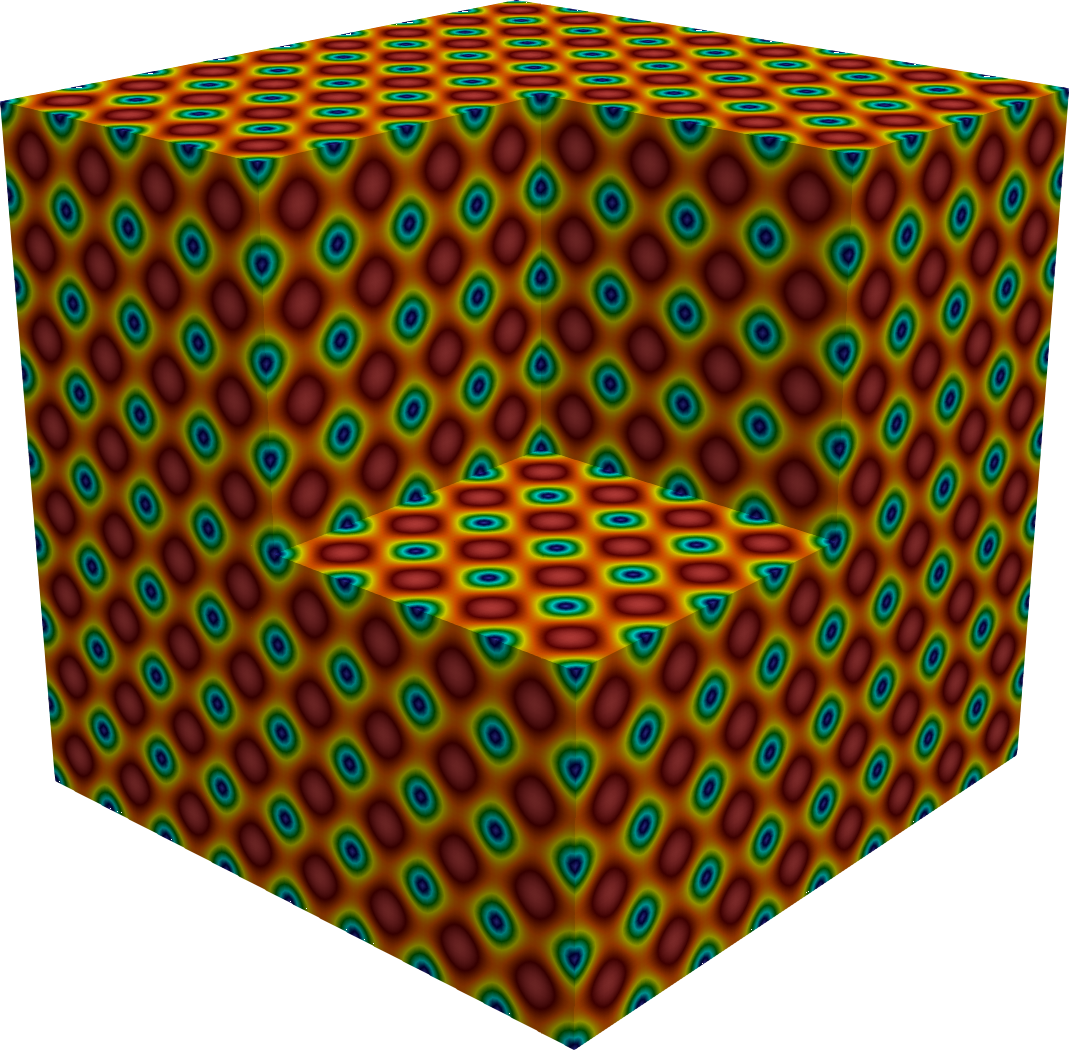
\includegraphics[width=0.45\textwidth]{Data/fichera.png}};
  \end{tikzpicture}
      \begin{tikzpicture}[overlay,remember picture]
      \begin{axis}[
              at=(fig.south west),
          xshift=-1.25cm,yshift=-2cm,
    enlargelimits=false,
    colorbar,
    colormap name=paraview,
    point meta min=0,
    point meta max=1.4,
    hide axis,
    colorbar style={
        ytick style={draw=none},
        title={$||E||$},
        scaled y ticks = false,
        height = 2.0cm,
        font = \tiny,
        width = 0.3cm,
        ytick={0,0.7,1.4}
    }
    ]
      \end{axis}
  \end{tikzpicture}
  }
    \subfloat[\parbox{5cm}{Convergence history of \pk{PCBDDC} using \pk{PCHPDDM}
    as a coarse solver.\label{fig:BDDC}}]{
        \begin{tikzpicture}[font=\scriptsize]
\begin{axis}[%title=\framebox{{\upcase diffusion 2D, $\mathbb{P}_4$ FE, $\varepsilon = \num[exponent-product=\cdot]{1e-06}$}},
        axis y line*=left,ymajorgrids, unbounded coords=jump, xmin=-1,extra y ticks={100}, width=0.5\textwidth,extra y tick labels=\empty, extra y tick style={grid=major}, ylabel = {\# of inner iterations~\ref{pgfplots:inner}}, xlabel = {Outer iteration index}]
\addplot[last, very thick] table[x=it, y=inner] {\loadedtableBDDC};\label{pgfplots:inner}
% \node[rectangle, draw, font=\scriptsize, text width = 4.6cm] at (axis cs:12.9, 18) {\texttt{-hpddm\_master\_p 32 \\ -hpddm\_master\_aggregate\_size 16}};
\end{axis}
\begin{semilogyaxis}[axis x line=none, axis y line*=right, xmin=-1,width=0.5\textwidth, ylabel near ticks=right, ylabel = {Unpreconditioned residual~\ref{pgfplots:res}}]
\addplot[myred, densely dashed, very thick] table[x=it, y=res] {\loadedtableBDDC};\label{pgfplots:res}
\end{semilogyaxis}
\end{tikzpicture}
  }
    \caption{MFEM example ex3p for solving the Fichera corner problem.}
\end{figure}
\section{Conclusion and perspectives}\label{sec:conclusion}
In this paper, the interface between PETSc and HPDDM is presented. The new
registered Krylov and overlapping Schwarz methods are explained and numerical
examples are provided to show the applicability of these. Solving well-known
problems, various options have been described. Some more unconventional test
cases were commented as well, for example using \pk{MatKAIJ} or \pk{MatIS} matrix types.
Overall, the interface paves the way for having recycling and block Krylov
methods plus robust overlapping Schwarz methods using the GenEO framework in
PETSc.

Concerning PETSc, the infrastructure for dealing with blocks of vectors has
been laid out. Still, only a little fraction of the built-in matrix types and
preconditioners may efficiently handle such a format.

Concerning HPDDM, its integration inside PETSc offers a much-needed flexibility
compared to the standard implementation. Indeed, it is now possible to switch at
runtime many parameters that are determined at compile-time in the standard implementation, e.g.,
subdomain solvers, matrix types, and such.


\section*{Acknowledgments}
The authors would like to thank S. Balay, J. Brown, V. Hapla, M. Knepley,
and B. Smith for reviewing the successive merge requests in the PETSc
repository. This work was granted access to the GENCI-sponsored HPC resources of:
\begin{itemize}
    \item TGCC@CEA under allocation A0070607519;
    \item IDRIS@CNRS under allocation AP010611780.
\end{itemize}
% We would like to acknowledge the assistance of volunteers in putting
% together this example manuscript and supplement.

\bibliographystyle{siamplain}
\begin{thebibliography}{10}

\bibitem{adams2004ultra}
{\sc M.~Adams, H.~H. Bayraktar, T.~M. Keaveny, and P.~Papadopoulos}, {\em
  {Ultrascalable Implicit Finite Element Analyses in Solid Mechanics with over
  a Half a Billion Degrees of Freedom}}, in Proceedings of the 2004 ACM/IEEE
  Conference on Supercomputing, SC04, IEEE Computer Society, 2004,
  pp.~\mbox{34:1--34:15}.

\bibitem{aldaas2019multi}
{\sc H.~Al~Daas, L.~Grigori, P.~Jolivet, and P.-H. Tournier}, {\em {A
  Multilevel Schwarz Preconditioner Based on a Hierarchy of Robust Coarse
  Spaces}}, Journal of Scientific Computing,  (2019), p.~submitted for
  publication, \url{https://github.com/prj-/aldaas2019multi}.

\bibitem{amestoy2001fully}
{\sc P.~Amestoy, I.~Duff, J.-Y. L'Excellent, and J.~Koster}, {\em A fully
  asynchronous multifrontal solver using distributed dynamic scheduling}, SIAM
  Journal on Matrix Analysis and Applications, 23 (2001), pp.~15--41,
  \url{http://mumps.enseeiht.fr}.

\bibitem{anderson2019mfem}
{\sc R.~Anderson, J.~Andrej, A.~Barker, J.~Bramwell, J.-S. Camier, J.~Cerveny,
  V.~Dobrev, Y.~Dudouit, A.~Fisher, T.~Kolev, et~al.}, {\em {MFEM: a modular
  finite element methods library}}, arXiv:1911.09220,  (2019),
  \url{http://mfem.org}.

\bibitem{badia2014highly}
{\sc S.~Badia, A.~F. Mart{\'\i}n, and J.~Principe}, {\em A highly scalable
  parallel implementation of balancing domain decomposition by constraints},
  SIAM Journal on Scientific Computing, 36 (2014), pp.~C190--C218.

\bibitem{baker2005technique}
{\sc A.~H. Baker, E.~R. Jessup, and T.~Manteuffel}, {\em {A Technique for
  Accelerating the Convergence of Restarted GMRES}}, SIAM Journal on Matrix
  Analysis and Applications, 26 (2005), pp.~962--984.

\bibitem{balay1997cient}
{\sc S.~Balay, W.~D. Gropp, L.~Curfman~McInnes, and B.~F. Smith}, {\em
  Efficient management of parallelism in object-oriented numerical software
  libraries}, Modern Software Tools in Scientific Computing,  (1997),
  pp.~163--202.

\bibitem{barrett1994templates}
{\sc R.~Barrett, M.~Berry, T.~F. Chan, J.~Demmel, J.~Donato, J.~Dongarra,
  V.~Eijkhout, R.~Pozo, C.~Romine, and H.~Van~der Vorst}, {\em Templates for
  the solution of linear systems: building blocks for iterative methods}, SIAM,
  1994.

\bibitem{Bartlett:2017:XFT}
{\sc R.~Bartlett, I.~Demeshko, T.~Gamblin, G.~Hammond, M.~A. Heroux,
  J.~Johnson, A.~Klinvex, X.~Li, L.~C. McInnes, J.~D. Moulton, D.~Osei-Kuffuor,
  J.~Sarich, B.~Smith, J.~Willenbring, and U.~M. Yang}, {\em {xSDK Foundations:
  Toward an Extreme-scale Scientific Software Development Kit}}, Supercomputing
  Frontiers and Innovations, 4 (2017).

\bibitem{bastian1998additive}
{\sc P.~Bastian, G.~Wittum, and W.~Hackbusch}, {\em Additive and multiplicative
  multi-grid—a comparison}, Computing, 60 (1998), pp.~345--364.

\bibitem{bavier2012amesos2}
{\sc E.~Bavier, M.~Hoemmen, S.~Rajamanickam, and H.~Thornquist}, {\em {Amesos2
  and Belos: Direct and Iterative Solvers for Large Sparse Linear Systems}},
  Scientific Programming, 20 (2012), pp.~241--255.

\bibitem{Benzi2011a}
{\sc M.~Benzi, M.~A. Olshanskii, and Z.~Wang}, {\em {Modified augmented
  Lagrangian preconditioners for the incompressible Navier--Stokes equations}},
  International Journal for Numerical Methods in Fluids, 66 (2011),
  pp.~486--508.

\bibitem{10.1145/3232850}
{\sc W.~Boukaram, G.~Turkiyyah, and D.~Keyes}, {\em {Hierarchical Matrix
  Operations on GPUs: Matrix-Vector Multiplication and Compression}}, ACM
  Transactions on Mathematical Software, 45 (2019).

\bibitem{brown2012composable}
{\sc J.~Brown, M.~G. Knepley, D.~A. May, L.~Curfman~McInnes, and B.~F. Smith},
  {\em Composable linear solvers for multiphysics}, in 2012 11th International
  Symposium on Parallel and Distributed Computing, IEEE, 2012, pp.~55--62.

\bibitem{BursteddeWilcoxGhattas11}
{\sc C.~Burstedde, L.~C. Wilcox, and O.~Ghattas}, {\em {\texttt{p4est}}:
  Scalable algorithms for parallel adaptive mesh refinement on forests of
  octrees}, SIAM Journal on Scientific Computing, 33 (2011), pp.~1103--1133,
  \url{http://www.p4est.org}.

\bibitem{butler2020high}
{\sc R.~Butler, T.~Dodwell, A.~Reinarz, A.~Sandhu, R.~Scheichl, and
  L.~Seelinger}, {\em High-performance dune modules for solving large-scale,
  strongly anisotropic elliptic problems with applications to aerospace
  composites}, Computer Physics Communications, 249 (2020).

\bibitem{cai1999restricted}
{\sc X.-C. Cai and M.~Sarkis}, {\em {A restricted additive Schwarz
  preconditioner for general sparse linear systems}}, SIAM Journal on
  Scientific Computing, 21 (1999), pp.~792--797.

\bibitem{calandra2012flexible}
{\sc H.~Calandra, S.~Gratton, J.~Langou, X.~Pinel, and X.~Vasseur}, {\em
  {Flexible Variants of Block Restarted GMRES Methods with Application to
  Geophysics}}, SIAM Journal on Scientific Computing, 34 (2012),
  pp.~A714--A736.

\bibitem{carvalho2011flexible}
{\sc L.~M. Carvalho, S.~Gratton, R.~Lago, and X.~Vasseur}, {\em {A Flexible
  Generalized Conjugate Residual Method With Inner Orthogonalization and
  Deflated Restarting}}, SIAM Journal on Matrix Analysis and Applications, 32
  (2011), pp.~1212--1235.

\bibitem{conen2014coarse}
{\sc L.~Conen, V.~Dolean, R.~Krause, and F.~Nataf}, {\em {A coarse space for
  heterogeneous Helmholtz problems based on the Dirichlet-to-Neumann
  operator}}, Journal of Computational and Applied Mathematics, 271 (2014),
  pp.~83--99.

\bibitem{da2014isogeometric}
{\sc L.~B. Da~Veiga, L.~F. Pavarino, S.~Scacchi, O.~B. Widlund, and
  S.~Zampini}, {\em {Isogeometric BDDC preconditioners with deluxe scaling}},
  SIAM Journal on Scientific Computing, 36 (2014), pp.~A1118--A1139.

\bibitem{davis2004algorithm}
{\sc T.~A. Davis}, {\em Algorithm 832: {UMFPACK}—an unsymmetric-pattern
  multifrontal method}, ACM Transactions on Mathematical Software, 30 (2004),
  pp.~196--199.

\bibitem{dolean2014ddm}
{\sc V.~Dolean, P.~Jolivet, and F.~Nataf}, {\em An Introduction to Domain
  Decomposition Methods\col\ Algorithms, Theory and Parallel Implementation},
  SIAM, 2015.

\bibitem{erhel1996restarted}
{\sc J.~Erhel, K.~Burrage, and B.~Pohl}, {\em {Restarted GMRES preconditioned
  by deflation}}, Journal of Computational and Applied Mathematics, 69 (1996),
  pp.~303--318.

\bibitem{falgout2002hypre}
{\sc R.~Falgout and U.~Yang}, {\em \emph{hypre}: a library of high performance
  preconditioners}, Computational Science---ICCS 2002,  (2002), pp.~632--641,
  \url{https://www.llnl.gov/casc/hypre}.

\bibitem{frommer2017block}
{\sc A.~Frommer, K.~Lund, and D.~B. Szyld}, {\em {Block Krylov Subspace Methods
  for Functions of Matrices}}, Electronic Transactions on Numerical Analysis,
  47 (2017), pp.~100--126.

\bibitem{gander2006optimized}
{\sc M.~J. Gander}, {\em Optimized {S}chwarz {M}ethods}, SIAM Journal on
  Numerical Analysis, 44 (2006), pp.~699--731.

\bibitem{gee2006ml}
{\sc M.~W. Gee, C.~M. Siefert, J.~J. Hu, R.~S. Tuminaro, and M.~G. Sala}, {\em
  {ML} 5.0 smoothed aggregation user's guide}, Tech. Report SAND2006-2649,
  Sandia National Laboratories, 2006, \url{https://trilinos.github.io/ml.html}.

\bibitem{gutknecht2006block}
{\sc M.~H. Gutknecht}, {\em Block {K}rylov space methods for linear systems
  with multiple right-hand sides: an introduction}, in Modern Mathematical
  Models, Methods and Algorithms for Real World Systems, A.~Siddiqui, I.~Duff,
  and O.~Christensen, eds., 2006, pp.~420--447.

\bibitem{gutknecht2008updating}
{\sc M.~H. Gutknecht and T.~Schmelzer}, {\em {Updating the $QR$ decomposition
  of block tridiagonal and block Hessenberg matrices}}, {Applied Numerical
  Mathematics}, 58 (2008), pp.~871--883.

\bibitem{haferssas2017soras}
{\sc R.~Haferssas, P.~Jolivet, and F.~Nataf}, {\em {An additive Schwarz method
  type theory for Lions's algorithm and a Symmetrized Optimized Restricted
  Additive Schwarz Method}}, Journal on Scientific Computing, 39 (2017),
  pp.~A1345--A1365.

\bibitem{hecht2012new}
{\sc F.~Hecht}, {\em New development in {FreeFem++}}, Journal of Numerical
  Mathematics, 20 (2012), pp.~251--266, \url{http://freefem.org}.

\bibitem{heinecke2016libxsmm}
{\sc A.~Heinecke, G.~Henry, M.~Hutchinson, and H.~Pabst}, {\em {LIBXSMM:
  accelerating small matrix multiplications by runtime code generation}}, in
  Proceedings of the 2016 International Conference for High Performance
  Computing, Networking, Storage and Analysis, SC16, IEEE, 2016,
  \url{https://github.com/hfp/libxsmm}.

\bibitem{Heinlein:2016:PIT}
{\sc A.~Heinlein, A.~Klawonn, and O.~Rheinbach}, {\em A parallel implementation
  of a two-level overlapping {S}chwarz method with energy-minimizing coarse
  space based on {T}rilinos}, SIAM Journal on Scientific Computing, 38 (2016),
  pp.~C713--C747.

\bibitem{hernandez2005ssf}
{\sc V.~Hernandez, J.~E. Roman, and V.~Vidal}, {\em {SLEP}c: A scalable and
  flexible toolkit for the solution of eigenvalue problems}, ACM Transactions
  on Mathematical Software, 31 (2005), pp.~351--362,
  \url{https://slepc.upv.es}.

\bibitem{heroux2005overview}
{\sc M.~A. Heroux, R.~A. Bartlett, V.~E. Howle, R.~J. Hoekstra, J.~J. Hu, T.~G.
  Kolda, R.~B. Lehoucq, K.~R. Long, R.~P. Pawlowski, E.~T. Phipps, et~al.},
  {\em {An overview of the Trilinos project}}, ACM Transactions on Mathematical
  Software (TOMS), 31 (2005), pp.~397--423, \url{https://trilinos.github.io}.

\bibitem{hestenes1952methods}
{\sc M.~R. Hestenes and E.~Stiefel}, {\em {Methods of Conjugate Gradients for
  Solving Linear Systems}}, Journal of Research of the National Bureau of
  Standards, 49 (1952), pp.~409--436.

\bibitem{hoefler2015scientific}
{\sc T.~Hoefler and R.~Belli}, {\em Scientific benchmarking of parallel
  computing systems: twelve ways to tell the masses when reporting performance
  results}, in Proceedings of the 2015 International Conference for High
  Performance Computing, Networking, Storage and Analysis, SC15, 2015.

\bibitem{mkl-web-page}
{\sc Intel}, {\em {MKL} web page}.
\newblock
  \url{https://software.intel.com/content/www/us/en/develop/tools/math-kernel-library.html},
  2020.

\bibitem{ji2017breakdown}
{\sc H.~Ji and Y.~Li}, {\em A breakdown-free block conjugate gradient method},
  BIT Numerical Mathematics, 57 (2017), pp.~379--403.

\bibitem{jolivet2013scalable}
{\sc P.~Jolivet, F.~Hecht, F.~Nataf, and C.~Prud'homme}, {\em {Scalable Domain
  Decomposition Preconditioners for Heterogeneous Elliptic Problems}}, in
  Proceedings of the International Conference on High Performance Computing,
  Networking, Storage and Analysis, SC13, ACM, 2013.

\bibitem{jolivet2016block}
{\sc P.~Jolivet and P.-H. Tournier}, {\em {Block Iterative Methods and
  Recycling for Improved Scalability of Linear Solvers}}, in Proceedings of the
  2016 International Conference for High Performance Computing, Networking,
  Storage and Analysis, SC16, IEEE, 2016.

\bibitem{KALANTZIS2018136}
{\sc V.~Kalantzis, A.~C.~I. Malossi, C.~Bekas, A.~Curioni, E.~Gallopoulos, and
  Y.~Saad}, {\em A scalable iterative dense linear system solver for multiple
  right-hand sides in data analytics}, Parallel Computing, 74 (2018),
  pp.~136--153.

\bibitem{karypis1998fast}
{\sc G.~Karypis and V.~Kumar}, {\em A fast and high quality multilevel scheme
  for partitioning irregular graphs}, SIAM Journal on Scientific Computing, 20
  (1998), pp.~359--392,
  \url{http://glaros.dtc.umn.edu/gkhome/metis/parmetis/overview}.

\bibitem{knepley2009mesh}
{\sc M.~G. Knepley and D.~A. Karpeev}, {\em {Mesh algorithms for PDE with Sieve
  I: Mesh distribution}}, Scientific Programming, 17 (2009), pp.~215--230.

\bibitem{knyazev2001toward}
{\sc A.~V. Knyazev}, {\em {Toward the optimal preconditioned eigensolver:
  Locally optimal block preconditioned conjugate gradient method}}, SIAM
  journal on scientific computing, 23 (2001), pp.~517--541.

\bibitem{li2005overview}
{\sc X.~S. Li}, {\em {An overview of SuperLU: Algorithms, implementation, and
  user interface}}, ACM Transactions on Mathematical Software, 31 (2005),
  pp.~302--325.

\bibitem{li2003superlu_dist}
{\sc X.~S. Li and J.~Demmel}, {\em {SuperLU\_DIST: A scalable
  distributed-memory sparse direct solver for unsymmetric linear systems}}, ACM
  Transactions on Mathematical Software, 29 (2003), pp.~110--140.

\bibitem{mandel1993balancing}
{\sc J.~Mandel}, {\em Balancing domain decomposition}, Communications in
  Numerical Methods in Engineering, 9 (1993), pp.~233--241.

\bibitem{marchand2019two}
{\sc P.~Marchand, X.~Claeys, P.~Jolivet, F.~Nataf, and P.-H. Tournier}, {\em
  {Two-level preconditioning for $h$-version boundary element approximation of
  hypersingular operator with GenEO}}, Numerische Mathematik,  (2019),
  p.~submitted for publication.

\bibitem{mathew2008domain}
{\sc T.~Mathew}, {\em Domain decomposition methods for the numerical solution
  of partial differential equations}, vol.~61, Springer Science \& Business
  Media, 2008.

\bibitem{may2016extreme}
{\sc D.~A. May, P.~Sanan, K.~Rupp, M.~G. Knepley, and B.~F. Smith}, {\em
  {Extreme-scale multigrid components within PETSc}}, in Proceedings of the
  Platform for Advanced Scientific Computing Conference, 2016.

\bibitem{moulin2018al}
{\sc J.~Moulin, P.~Jolivet, and O.~Marquet}, {\em {Augmented Lagrangian
  Preconditioner for Large-Scale Hydrodynamic Stability Analysis}}, Computer
  Methods in Applied Mechanics and Engineering, 351 (2019), pp.~718--743,
  \url{https://github.com/prj-/moulin2019al}.

\bibitem{notay2000flexible}
{\sc Y.~Notay}, {\em Flexible conjugate gradients}, SIAM Journal on Scientific
  Computing, 22 (2000), pp.~1444--1460.

\bibitem{cusparse-web-page}
{\sc NVIDIA}, {\em {cuSPARSE} web page}.
\newblock \url{https://docs.nvidia.com/cuda/cusparse/}, 2020.

\bibitem{oh2018bddc}
{\sc D.-S. Oh, O.~B. Widlund, S.~Zampini, and C.~Dohrmann}, {\em {BDDC
  algorithms with deluxe scaling and adaptive selection of primal constraints
  for Raviart--Thomas vector fields}}, Mathematics of Computation, 87 (2018),
  pp.~659--692.

\bibitem{o1980block}
{\sc D.~P. O'Leary}, {\em {The Block Conjugate Gradient Algorithm and Related
  Methods}}, Linear Algebra and its Applications, 29 (1980), pp.~293--322.

\bibitem{parks2006recycling}
{\sc M.~L. Parks, E.~de~Sturler, G.~Mackey, D.~D. Johnson, and S.~Maiti}, {\em
  {Recycling Krylov Subspaces for Sequences of Linear Systems}}, SIAM Journal
  on Scientific Computing, 28 (2006), pp.~1651--1674.

\bibitem{pechstein2012finite}
{\sc C.~Pechstein}, {\em {Finite and Boundary Element Tearing and
  Interconnecting Solvers for Multiscale Problems}}, vol.~90 of Lecture Notes
  in Computational Science and Engineering, Springer, 2012.

\bibitem{pechstein2017unified}
{\sc C.~Pechstein and C.~R. Dohrmann}, {\em {A unified framework for adaptive
  BDDC}}, Electronic Transactions on Numerical Analysis, 46 (2017),
  pp.~273--336.

\bibitem{poulson2013elemental}
{\sc J.~Poulson, B.~Marker, R.~A. Van~de Geijn, J.~R. Hammond, and N.~A.
  Romero}, {\em {Elemental: A new framework for distributed memory dense matrix
  computations}}, ACM Transactions on Mathematical Software, 39 (2013).

\bibitem{quarteroni1999domain}
{\sc A.~Quarteroni and A.~Valli}, {\em Domain decomposition methods for partial
  differential equations}, vol.~10, Clarendon Press, 1999.

\bibitem{saad1993flexible}
{\sc Y.~Saad}, {\em {A Flexible Inner--Outer Preconditioned GMRES Algorithm}},
  SIAM Journal on Scientific Computing, 14 (1993), pp.~461--469.

\bibitem{saad2003iterative}
{\sc Y.~Saad}, {\em {Iterative Methods for Sparse Linear Systems, Second
  Edition}}, SIAM, 2003.

\bibitem{saad1986gmres}
{\sc Y.~Saad and M.~H. Schultz}, {\em {GMRES: a generalized minimal residual
  algorithm for solving nonsymmetric linear systems}}, SIAM Journal on
  Scientific and Statistical Computing, 7 (1986), pp.~856--869.

\bibitem{saad2000deflated}
{\sc Y.~Saad, M.~Yeung, J.~Erhel, and F.~Guyomarc'h}, {\em A deflated version
  of the conjugate gradient algorithm}, SIAM Journal on Scientific Computing,
  21 (2000), pp.~1909--1926.

\bibitem{sakurai2003projection}
{\sc T.~Sakurai and H.~Sugiura}, {\em A projection method for generalized
  eigenvalue problems using numerical integration}, Journal of Computational
  and Applied Mathematics, 159 (2003), pp.~119--128.

\bibitem{sakurai2010application}
{\sc T.~Sakurai, H.~Tadano, and Y.~Kuramashi}, {\em {Application of block
  Krylov subspace algorithms to the Wilson--Dirac equation with multiple
  right-hand sides in lattice QCD}}, Computer Physics Communications, 181
  (2010), pp.~113--117.

\bibitem{si2013tet}
{\sc H.~Si}, {\em {TetGen: A Quality Tetrahedral Mesh Generator and 3D Delaunay
  Triangulator}}, Tech. Report~13, 2013,
  \url{http://wias-berlin.de/software/tetgen}.

\bibitem{vsistek2013parallel}
{\sc J.~{\v{S}}{\'\i}stek, J.~Mandel, B.~Soused{\'\i}k, and P.~Burda}, {\em
  Parallel implementation of multilevel {BDDC}}, in Numerical Mathematics and
  Advanced Applications 2011, Springer, 2013, pp.~681--689,
  \url{http://users.math.cas.cz/~sistek/software/bddcml.html}.

\bibitem{smith2004domain}
{\sc B.~F. Smith, P.~Bj{\o}rstad, and W.~Gropp}, {\em Domain decomposition:
  parallel multilevel methods for elliptic partial differential equations},
  Cambridge University Press, 2004.

\bibitem{soodhalter2014krylov}
{\sc K.~M. Soodhalter, D.~B. Szyld, and F.~Xue}, {\em Krylov subspace recycling
  for sequences of shifted linear systems}, Applied Numerical Mathematics, 81
  (2014), pp.~105--118.

\bibitem{spillane2011robust}
{\sc N.~Spillane, V.~Dolean, P.~Hauret, F.~Nataf, C.~Pechstein, and
  R.~Scheichl}, {\em A robust two-level domain decomposition preconditioner for
  systems of {PDE}s}, Comptes Rendus Mathématique, 349 (2011), pp.~1255--1259.

\bibitem{spillane2013abstract}
{\sc N.~Spillane, V.~Dolean, P.~Hauret, F.~Nataf, C.~Pechstein, and
  R.~Scheichl}, {\em Abstract robust coarse spaces for systems of {PDEs} via
  generalized eigenproblems in the overlaps}, Numerische Mathematik, 126
  (2013), pp.~741--700.

\bibitem{spillane2013automatic}
{\sc N.~Spillane and D.~J. Rixen}, {\em Automatic spectral coarse spaces for
  robust finite element tearing and interconnecting and balanced domain
  decomposition algorithms}, International Journal for Numerical Methods in
  Engineering, 95 (2013), pp.~953--990.

\bibitem{stathopoulos2009deflation}
{\sc A.~Stathopoulos, A.~Abdel-Rehim, and K.~Orginos}, {\em {Deflation for
  inversion with multiple right-hand sides in QCD}}, in Journal of Physics:
  Conference Series, vol.~180, IOP Publishing, 2009.

\bibitem{stathopoulos2002block}
{\sc A.~Stathopoulos and K.~Wu}, {\em {A Block Orthogonalization Procedure with
  Constant Synchronization Requirements}}, SIAM Journal on Scientific
  Computing, 23 (2002), pp.~2165--2182.

\bibitem{Stewart2002}
{\sc G.~W. Stewart}, {\em {A Krylov--Schur Algorithm for Large Eigenproblems}},
  SIAM Journal on Matrix Analysis and Applications, 23 (2002), pp.~601--614.

\bibitem{tang2009comparison}
{\sc J.~Tang, R.~Nabben, C.~Vuik, and Y.~Erlangga}, {\em Comparison of
  two-level preconditioners derived from deflation, domain decomposition and
  multigrid methods}, Journal of Scientific Computing, 39 (2009), pp.~340--370.

\bibitem{toselli2005domain}
{\sc A.~Toselli and O.~B. Widlund}, {\em Domain decomposition methods:
  algorithms and theory}, vol.~34 of Series in Computational Mathematics,
  Springer, 2005.

\bibitem{tournier2016micro}
{\sc P.-H. Tournier, I.~Aliferis, M.~Bonazzoli, M.~de~Buhan, M.~Darbas,
  V.~Dolean, F.~Hecht, P.~Jolivet, I.~El~Kanfoud, C.~Migliaccio, F.~Nataf,
  C.~Pichot, and S.~Semenov}, {\em {Microwave Tomographic Imaging of
  Cerebrovascular Accidents by Using High-Performance Computing}}, Parallel
  Computing, 85 (2019), pp.~88--97.

\bibitem{van1992bi}
{\sc H.~A. Van~der Vorst}, {\em {Bi-CGSTAB: a fast and smoothly converging
  variant of Bi-CG for the solution of nonsymmetric linear systems}}, SIAM
  Journal on Scientific and Statistical Computing, 13 (1992), pp.~631--644.

\bibitem{wakam2013158}
{\sc D.~N. Wakam and F.~Pacull}, {\em Memory efficient hybrid algebraic solvers
  for linear systems arising from compressible flows}, Computers \& Fluids, 80
  (2013), pp.~158--167.

\bibitem{zampini2016pcbddc}
{\sc S.~Zampini}, {\em {PCBDDC: a class of robust dual--primal methods in
  PETSc}}, SIAM Journal on Scientific Computing, 38 (2016), pp.~S282--S306,
  \url{https://www.mcs.anl.gov/petsc/petsc-master/docs/manualpages/PC/PCBDDC.html}.

\bibitem{zampini2017balancing}
{\sc S.~Zampini, P.~Vassilevski, V.~Dobrev, and T.~Kolev}, {\em {Balancing
  Domain Decomposition by Constraints Algorithms for Curl-Conforming Spaces of
  Arbitrary Order}}, in International Conference on Domain Decomposition
  Methods, Springer, 2017, pp.~103--116.

\end{thebibliography}
\end{document}
